\documentclass[]{tufte-book}

% ams
\usepackage{amssymb,amsmath}

\usepackage{ifxetex,ifluatex}
\usepackage{fixltx2e} % provides \textsubscript
\ifnum 0\ifxetex 1\fi\ifluatex 1\fi=0 % if pdftex
  \usepackage[T1]{fontenc}
  \usepackage[utf8]{inputenc}
\else % if luatex or xelatex
  \makeatletter
  \@ifpackageloaded{fontspec}{}{\usepackage{fontspec}}
  \makeatother
  \defaultfontfeatures{Ligatures=TeX,Scale=MatchLowercase}
  \makeatletter
  \@ifpackageloaded{soul}{
     \renewcommand\allcapsspacing[1]{{\addfontfeature{LetterSpace=15}#1}}
     \renewcommand\smallcapsspacing[1]{{\addfontfeature{LetterSpace=10}#1}}
   }{}
  \makeatother
\fi

% graphix
\usepackage{graphicx}
\setkeys{Gin}{width=\linewidth,totalheight=\textheight,keepaspectratio}

% booktabs
\usepackage{booktabs}

% url
\usepackage{url}

% hyperref
\usepackage{hyperref}

% units.
\usepackage{units}


\setcounter{secnumdepth}{2}

% citations
\usepackage{natbib}
\bibliographystyle{apalike}

% pandoc syntax highlighting
\usepackage{color}
\usepackage{fancyvrb}
\newcommand{\VerbBar}{|}
\newcommand{\VERB}{\Verb[commandchars=\\\{\}]}
\DefineVerbatimEnvironment{Highlighting}{Verbatim}{commandchars=\\\{\}}
% Add ',fontsize=\small' for more characters per line
\usepackage{framed}
\definecolor{shadecolor}{RGB}{248,248,248}
\newenvironment{Shaded}{\begin{snugshade}}{\end{snugshade}}
\newcommand{\KeywordTok}[1]{\textcolor[rgb]{0.13,0.29,0.53}{\textbf{{#1}}}}
\newcommand{\DataTypeTok}[1]{\textcolor[rgb]{0.13,0.29,0.53}{{#1}}}
\newcommand{\DecValTok}[1]{\textcolor[rgb]{0.00,0.00,0.81}{{#1}}}
\newcommand{\BaseNTok}[1]{\textcolor[rgb]{0.00,0.00,0.81}{{#1}}}
\newcommand{\FloatTok}[1]{\textcolor[rgb]{0.00,0.00,0.81}{{#1}}}
\newcommand{\ConstantTok}[1]{\textcolor[rgb]{0.00,0.00,0.00}{{#1}}}
\newcommand{\CharTok}[1]{\textcolor[rgb]{0.31,0.60,0.02}{{#1}}}
\newcommand{\SpecialCharTok}[1]{\textcolor[rgb]{0.00,0.00,0.00}{{#1}}}
\newcommand{\StringTok}[1]{\textcolor[rgb]{0.31,0.60,0.02}{{#1}}}
\newcommand{\VerbatimStringTok}[1]{\textcolor[rgb]{0.31,0.60,0.02}{{#1}}}
\newcommand{\SpecialStringTok}[1]{\textcolor[rgb]{0.31,0.60,0.02}{{#1}}}
\newcommand{\ImportTok}[1]{{#1}}
\newcommand{\CommentTok}[1]{\textcolor[rgb]{0.56,0.35,0.01}{\textit{{#1}}}}
\newcommand{\DocumentationTok}[1]{\textcolor[rgb]{0.56,0.35,0.01}{\textbf{\textit{{#1}}}}}
\newcommand{\AnnotationTok}[1]{\textcolor[rgb]{0.56,0.35,0.01}{\textbf{\textit{{#1}}}}}
\newcommand{\CommentVarTok}[1]{\textcolor[rgb]{0.56,0.35,0.01}{\textbf{\textit{{#1}}}}}
\newcommand{\OtherTok}[1]{\textcolor[rgb]{0.56,0.35,0.01}{{#1}}}
\newcommand{\FunctionTok}[1]{\textcolor[rgb]{0.00,0.00,0.00}{{#1}}}
\newcommand{\VariableTok}[1]{\textcolor[rgb]{0.00,0.00,0.00}{{#1}}}
\newcommand{\ControlFlowTok}[1]{\textcolor[rgb]{0.13,0.29,0.53}{\textbf{{#1}}}}
\newcommand{\OperatorTok}[1]{\textcolor[rgb]{0.81,0.36,0.00}{\textbf{{#1}}}}
\newcommand{\BuiltInTok}[1]{{#1}}
\newcommand{\ExtensionTok}[1]{{#1}}
\newcommand{\PreprocessorTok}[1]{\textcolor[rgb]{0.56,0.35,0.01}{\textit{{#1}}}}
\newcommand{\AttributeTok}[1]{\textcolor[rgb]{0.77,0.63,0.00}{{#1}}}
\newcommand{\RegionMarkerTok}[1]{{#1}}
\newcommand{\InformationTok}[1]{\textcolor[rgb]{0.56,0.35,0.01}{\textbf{\textit{{#1}}}}}
\newcommand{\WarningTok}[1]{\textcolor[rgb]{0.56,0.35,0.01}{\textbf{\textit{{#1}}}}}
\newcommand{\AlertTok}[1]{\textcolor[rgb]{0.94,0.16,0.16}{{#1}}}
\newcommand{\ErrorTok}[1]{\textcolor[rgb]{0.64,0.00,0.00}{\textbf{{#1}}}}
\newcommand{\NormalTok}[1]{{#1}}

% longtable
\usepackage{longtable,booktabs}

% multiplecol
\usepackage{multicol}

% strikeout
\usepackage[normalem]{ulem}

% morefloats
\usepackage{morefloats}


% tightlist macro required by pandoc >= 1.14
\providecommand{\tightlist}{%
  \setlength{\itemsep}{0pt}\setlength{\parskip}{0pt}}

% title / author / date
\title{\Large{A MODERN DIVE into Data with R}}
\author{Chester Ismay}
\date{2016-08-29}

\usepackage{booktabs}
\usepackage{longtable}
\usepackage{framed,color}
\definecolor{shadecolor}{RGB}{248,248,248}

\ifxetex
  \usepackage{letltxmacro}
  \setlength{\XeTeXLinkMargin}{1pt}
  \LetLtxMacro\SavedIncludeGraphics\includegraphics
  \def\includegraphics#1#{% #1 catches optional stuff (star/opt. arg.)
    \IncludeGraphicsAux{#1}%
  }%
  \newcommand*{\IncludeGraphicsAux}[2]{%
    \XeTeXLinkBox{%
      \SavedIncludeGraphics#1{#2}%
    }%
  }%
\fi

%% Need to clean up
\newenvironment{rmdblock}[1]
  {\begin{shaded*}
  \begin{itemize}
  \renewcommand{\labelitemi}{
    \raisebox{-.7\height}[0pt][0pt]{
  %    {\setkeys{Gin}{width=3em,keepaspectratio}\includegraphics{images/#1}}
    }
  }
  \item
  }
  {
  \end{itemize}
  \end{shaded*}
  }
%% Probably can be omitted
\newenvironment{rmdnote}
  {\begin{rmdblock}{note}}
  {\end{rmdblock}}
\newenvironment{rmdcaution}
  {\begin{rmdblock}{caution}}
  {\end{rmdblock}}
\newenvironment{rmdimportant}
  {\begin{rmdblock}{important}}
  {\end{rmdblock}}
\newenvironment{rmdtip}
  {\begin{rmdblock}{tip}}
  {\end{rmdblock}}
\newenvironment{rmdwarning}
  {\begin{rmdblock}{warning}}
  {\end{rmdblock}}
\newenvironment{learncheck}
  {\begin{rmdblock}{warning}}
  {\end{rmdblock}}
\newenvironment{review}
  {\begin{rmdblock}{warning}}
  {\end{rmdblock}}

% To tweak tufte layout
\geometry{
  left=0.8in, % left margin
  textwidth=35pc, % main text block
  marginparsep=1pc, % gutter between main text block and margin notes
  marginparwidth=8pc % width of margin notes
}

\begin{document}

\maketitle



{
\setcounter{tocdepth}{1}
\tableofcontents
}

\chapter{Prerequisites}\label{prereqs}

This book was written using the \textbf{bookdown} R package from Yihui
Xie. In order to follow along and run the code in this book on your own,
you'll need to have access to R and RStudio. You can find more
information on both of these with a simple Google search for ``R'' and
for ``RStudio.'' An introduction to using R, RStudio, and R Markdown is
also available in a free book
\href{http://ismayc.github.io/rbasics-book}{here} \citep{usedtor2016}.
It is recommended that you refer back to this book frequently as it has
GIF screen recordings that you can follow along with as you learn.

We will keep a running list of R packages you will need to have
installed to complete the analysis as well here in the
\texttt{needed\_pkgs} character vector. You can check if you have all of
the needed packages installed by running all of the lines below. The
last lines including the \texttt{if} will install them as needed (i.e.,
download their needed files from the internet to your hard drive).

You can run the \texttt{library} function on them to load them into your
current analysis. Prior to each analysis where a package is needed, you
will see the corresponding \texttt{library} function in the text. Make
sure to check the top of the chapter to see if a package was loaded
there.

\begin{Shaded}
\begin{Highlighting}[]
\NormalTok{needed_pkgs <-}\StringTok{ }\KeywordTok{c}\NormalTok{(}\StringTok{"nycflights13"}\NormalTok{, }\StringTok{"dplyr"}\NormalTok{, }\StringTok{"ggplot2"}\NormalTok{, }\StringTok{"knitr"}\NormalTok{, }
  \StringTok{"ggplot2movies"}\NormalTok{, }\StringTok{"dygraphs"}\NormalTok{, }\StringTok{"rmarkdown"}\NormalTok{, }\StringTok{"mosaic"}\NormalTok{, }\StringTok{"tibble"}\NormalTok{)}

\NormalTok{new.pkgs <-}\StringTok{ }\NormalTok{needed_pkgs[!(needed_pkgs %in%}\StringTok{ }\KeywordTok{installed.packages}\NormalTok{())]}

\NormalTok{if(}\KeywordTok{length}\NormalTok{(new.pkgs)) \{}
  \KeywordTok{install.packages}\NormalTok{(new.pkgs, }\DataTypeTok{repos =} \StringTok{"http://cran.rstudio.com"}\NormalTok{)}
\NormalTok{\}}
\end{Highlighting}
\end{Shaded}

\textbf{Book was last updated:}

\begin{verbatim}
## [1] "By Chester on Monday, August 29, 2016 13:18:46 PDT"
\end{verbatim}

\section{Colophon}\label{colophon}

The source of the book is available
\href{https://github.com/ModernStats/bookdown}{here} and was built with
versions of R packages given below. This may not be of importance for
initial readers of this book, but the hope is you can reproduce a
duplicate of this book by installing these versions of the packages.

\begin{longtable}{lllll}
\toprule
package & * & version & date & source\\
\midrule
assertthat &  & 0.1 & 2013-12-06 & CRAN (R 3.3.0)\\
base64enc &  & 0.1-3 & 2015-07-28 & CRAN (R 3.3.0)\\
BH &  & 1.60.0-2 & 2016-05-07 & CRAN (R 3.3.0)\\
bitops &  & 1.0-6 & 2013-08-17 & CRAN (R 3.3.0)\\
caTools &  & 1.17.1 & 2014-09-10 & CRAN (R 3.3.0)\\
\addlinespace
colorspace &  & 1.2-6 & 2015-03-11 & CRAN (R 3.3.0)\\
curl &  & 1.2 & 2016-08-13 & CRAN (R 3.3.0)\\
DBI &  & 0.5 & 2016-08-11 & CRAN (R 3.3.0)\\
dichromat &  & 2.0-0 & 2013-01-24 & CRAN (R 3.3.0)\\
digest &  & 0.6.10 & 2016-08-02 & CRAN (R 3.3.0)\\
\addlinespace
dplyr &  & 0.5.0 & 2016-06-24 & CRAN (R 3.3.0)\\
dygraphs &  & 1.1.1-1 & 2016-08-06 & CRAN (R 3.3.0)\\
evaluate &  & 0.9 & 2016-04-29 & CRAN (R 3.3.0)\\
formatR &  & 1.4 & 2016-05-09 & CRAN (R 3.3.0)\\
ggdendro &  & 0.1-20 & 2016-04-27 & CRAN (R 3.3.0)\\
\addlinespace
ggplot2 &  & 2.1.0 & 2016-03-01 & CRAN (R 3.3.0)\\
ggplot2movies &  & 0.0.1 & 2015-08-25 & CRAN (R 3.3.0)\\
gridExtra &  & 2.2.1 & 2016-02-29 & CRAN (R 3.3.0)\\
gtable &  & 0.2.0 & 2016-02-26 & CRAN (R 3.3.0)\\
highr &  & 0.6 & 2016-05-09 & CRAN (R 3.3.0)\\
\addlinespace
hms &  & 0.2 & 2016-06-17 & CRAN (R 3.3.0)\\
htmltools &  & 0.3.5 & 2016-03-21 & CRAN (R 3.3.0)\\
htmlwidgets &  & 0.7 & 2016-08-02 & CRAN (R 3.3.0)\\
jsonlite &  & 1.0 & 2016-07-01 & CRAN (R 3.3.0)\\
knitr &  & 1.14 & 2016-08-13 & CRAN (R 3.3.0)\\
\addlinespace
labeling &  & 0.3 & 2014-08-23 & CRAN (R 3.3.0)\\
lattice &  & 0.20-33 & 2015-07-14 & CRAN (R 3.3.1)\\
latticeExtra &  & 0.6-28 & 2016-02-09 & CRAN (R 3.3.0)\\
lazyeval &  & 0.2.0 & 2016-06-12 & CRAN (R 3.3.0)\\
magrittr &  & 1.5 & 2014-11-22 & CRAN (R 3.3.0)\\
\addlinespace
markdown &  & 0.7.7 & 2015-04-22 & CRAN (R 3.3.0)\\
MASS &  & 7.3-45 & 2016-04-21 & CRAN (R 3.3.1)\\
Matrix &  & 1.2-6 & 2016-05-02 & CRAN (R 3.3.1)\\
mime &  & 0.5 & 2016-07-07 & CRAN (R 3.3.0)\\
mosaic &  & 0.14.4 & 2016-07-29 & CRAN (R 3.3.0)\\
\addlinespace
mosaicData &  & 0.14.0 & 2016-06-17 & CRAN (R 3.3.0)\\
munsell &  & 0.4.3 & 2016-02-13 & CRAN (R 3.3.0)\\
nycflights13 &  & 0.2.0 & 2016-04-30 & CRAN (R 3.3.0)\\
plyr &  & 1.8.4 & 2016-06-08 & CRAN (R 3.3.0)\\
R6 &  & 2.1.3 & 2016-08-19 & CRAN (R 3.3.0)\\
\addlinespace
RColorBrewer &  & 1.1-2 & 2014-12-07 & CRAN (R 3.3.0)\\
Rcpp &  & 0.12.6 & 2016-07-19 & CRAN (R 3.3.0)\\
readr &  & 1.0.0 & 2016-08-03 & CRAN (R 3.3.0)\\
reshape2 &  & 1.4.1 & 2014-12-06 & CRAN (R 3.3.0)\\
rmarkdown &  & 1.0 & 2016-07-08 & CRAN (R 3.3.0)\\
\addlinespace
scales &  & 0.4.0 & 2016-02-26 & CRAN (R 3.3.0)\\
stringi &  & 1.1.1 & 2016-05-27 & CRAN (R 3.3.0)\\
stringr &  & 1.1.0 & 2016-08-19 & CRAN (R 3.3.0)\\
tibble &  & 1.1 & 2016-07-04 & CRAN (R 3.3.0)\\
tidyr &  & 0.6.0 & 2016-08-12 & CRAN (R 3.3.0)\\
\addlinespace
xts &  & 0.9-7 & 2014-01-02 & CRAN (R 3.3.0)\\
yaml &  & 2.1.13 & 2014-06-12 & CRAN (R 3.3.0)\\
zoo &  & 1.7-13 & 2016-05-03 & CRAN (R 3.3.0)\\
\bottomrule
\end{longtable}

\chapter{Introduction}\label{intro}

\section{Preamble}\label{preamble}

This book is inspired by three books:

\begin{itemize}
\tightlist
\item
  ``Mathematical Statistics with Resampling and R'' \citep{hester2011},
\item
  ``Intro Stat with Randomization and Simulation'' \citep{isrs2014}, and
\item
  ``R for Data Science'' \citep{rds2016}.
\end{itemize}

The first book, while designed for upper-level undergraduates and
graduate students, provides an excellent resource on how to use
resampling to build statistical concepts like normal distributions using
computers instead of focusing on memorization of formulas. The last two
books also provide a path towards free alternatives to the traditionally
expensive introductory statistics textbook. When looking over the vast
number of introductory statistics textbooks we found that there wasn't
one that incorporated many of the new R packages directly into the text.
Additionally, there wasn't an open-source, free textbook available that
showed new learners all of the following

\begin{enumerate}
\def\labelenumi{\arabic{enumi}.}
\tightlist
\item
  how to use R to explore and visualize data
\item
  how to use randomization and simulation to build inferential ideas
\item
  how to effectively create stories using these ideas to convey
  information to a lay audience.
\end{enumerate}

We will introduce sometimes difficult statistics concepts through the
medium of data visualization. In today's world, we are bombarded with
graphics that attempt to convey ideas. We will explore what makes a good
graphic and what the standard ways are to convey relationships with
data. You'll also see the use of visualization to introduce concepts
like mean, median, standard deviation, distributions, etc. In general,
we'll use visualization as a way of building almost all of the ideas in
this book.

Additionally, this book will focus on the triad of computational
thinking, data thinking, and inferential thinking. We'll see throughout
the book how these three modes of thinking can build effective ways to
work with, describe, and convey statistical knowledge. In order to do
so, you'll see the importance of literate programming to develop
literate data science. In other words, you'll see how to write code and
descriptions that are useful not just for a computer to execute but also
for readers to understand exactly what a statistical analysis is doing
and how it works. Hal Abelson coined the phrase that we will follow
throughout this book:

\begin{quote}
``Programs must be written for people to read, and only incidentally for
machines to execute.''
\end{quote}

\section{Two driving data sources}\label{two-driving-data-sources}

Instead of hopping from one data set to the next, we've decided to focus
throughout the book on two different data sources: flights leaving New
York City in 2013 and IMDB (Internet Movie DataBase) ratings on movies.
By focusing on just two large data sources, it is our hope that you'll
be able to see how each of the chapters is interconnected. You'll see
how the data being tidy leads into data visualization and manipulation
and how those concepts tie into inference and regression.

\section{Data/science pipeline}\label{datascience-pipeline}

You may think of statistics as just being a bunch of numbers. We
commonly hear the phrase ``statistician'' when listening to broadcasts
of sporting events. Statistics (in particular, data analysis), in
addition to describing numbers like with baseball batting averages,
plays a vital role in all of the sciences. You'll commonly hear the
phrase ``statistically significant'' thrown around in the media. You'll
see things that say ``Science now shows that chocolate is good for
you.'' Underpinning these claims is data analysis. By the end of this
book, you'll be able to better understand whether these claims should be
trusted or whether we should be weary. Inside data analysis are many
sub-fields that we will discuss throughout this book (not necessarily in
this order):

\begin{itemize}
\tightlist
\item
  data collection
\item
  data manipulation
\item
  data visualization
\item
  data modeling
\item
  inference
\item
  interpretation of results
\item
  data storytelling
\end{itemize}

This can be summarized in a graphic that is commonly used by Hadley
Wickham:

\begin{figure}

{\centering 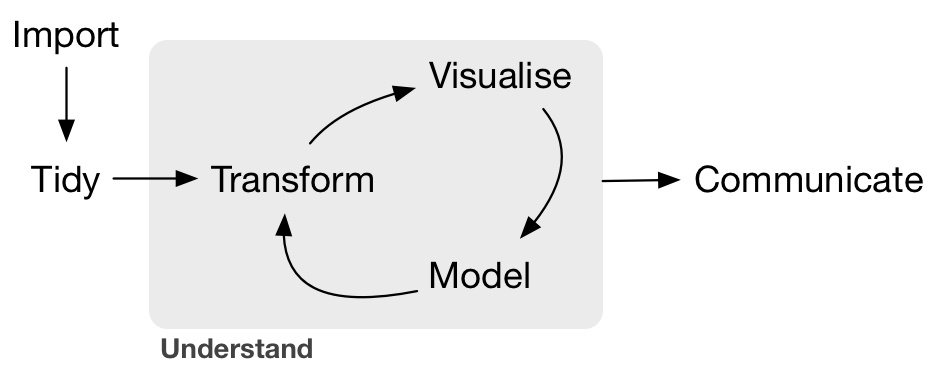
\includegraphics[width=\textwidth]{images/tidy1} 

}

\caption[Hadley's workflow graphic]{Hadley's workflow graphic}\label{fig:unnamed-chunk-4}
\end{figure}

We will begin with a discussion on what is meant by tidy data and then
dig into the gray \textbf{Understand} portion of the cycle and conclude
by talking about interpretting and discussing the results of our models
via \textbf{Communication}. These steps are vital to any statistical
analysis. But why should you care about statistics? ``Why did they make
me take this class?''

There's a reason so many fields require a statistics course. Scientific
knowledge grows through an understanding of statistical significance and
data analysis. You needn't be intimidated by statistics. It's not the
beast that it used to be and paired with computation you'll see how
reproducible research in the sciences particularly increases scientific
knowledge.

\section{Reproducibility}\label{reproducibility}

\begin{quote}
``The most important tool is the \emph{mindset}, when starting, that the
end product will be reproducible.'' -- Keith Baggerly
\end{quote}

Another large goal of this book is to help readers understand the
importance of reproducible analyses. The hope is to get readers into the
habit of making their analyses reproducible from the very beginning.
This means we'll be trying to help you build new habits. This will take
practice and be difficult at times. You'll see just why it is so
important for you to keep track of your code and well-document it to
help yourself later and any potential collaborators as well.

Copying and pasting is not the way that efficient and effective
scientific research is conducted. It's much more important for time to
be spent on data collection and data analysis and not on copying and
pasting plots back and forth across a variety of programs.

In a traditional analyses if an error was made with the original data,
we'd need to step through the entire process again: recreate the plots
and copy and paste all of the new plots and our statistical analsis into
your document. This is error prone and a frustrating use of time. We'll
see how to use R Markdown to get away from this tedious activity so that
we can spend more time doing science.

\begin{quote}
``We are talking about \emph{computational} reproducibility.'' - Yihui
Xie
\end{quote}

Reproducibility means a lot of things in terms of different scientific
fields. Are experiments conducted in a way that another researcher could
follow the steps and get similar results? In this book, we will focus on
what is known as \textbf{computational reproducibility}. This refers to
being able to pass all of one's data analysis and conclusions to someone
else and have them get exactly the same results on their machine. This
allows for time to be spent doing actual science and interpretting of
results and assumptions instead of the more error prone way of starting
from scratch or follow a list of steps that may be different from
machine to machine.

\section{Who is this book for?}\label{who-is-this-book-for}

This book is targetted at students taking a traditional intro stats
class in a small college environment using RStudio and preferably
RStudio Server. We assume no prerequisites: no calculus and no prior
programming experience. This is intended to be a gentle and nice
introduction to the practice of statistics in terms of how data
scientists, statisticians, and other scientists analyze data and write
stories about data. We have intentionally avoided the use of throwing
formulas at you and instead have focused on developing statistical
concepts via data visualization and statistical computing. We hope this
is a more intuitive experience than the way statistics has traditionally
been taught in the past (and how it is commonly perceived from the
outside). We additionally hope that you see the value of reproducible
research via R as you continue in your studies. We understand that there
will initially be growing pains in learning to program but we are here
to help you and you should know that there is a huge community of R
users that are always happy to help newbies along.

Now let's get into learning about how to create good stories about and
with data!

\part{Data Exploration}\label{part-data-exploration}


\chapter{Tidy data}\label{tidy}

In this chapter, we'll discuss the importance of tidy data. You may
think that this means just having your data in a spreadsheet, but you'll
see that it is actually more specific than that. Data actually comes to
us in a variety of formats from pictures to text and to just numbers.
We'll focus on datasets that can be stored in a spreadsheet throughout
this book as that is the most common way data is collected in the
sciences.

Having tidy data will allow us to more easily create data visualizations
as we will see in Chapter \ref{viz}. It will also help us with
manipulating data in Chapter \ref{manip} and in all subsequent chapters
when we discuss statistical inference. You may not necessarily
understand the importance for \textbf{tidy data} but it will become more
and more apparent as we proceed through the book.

\section{What is tidy data?}\label{what-is-tidy-data}

You have surely heard the word ``tidy'' in your life:

\begin{itemize}
\tightlist
\item
  ``Tidy up your room!''
\item
  ``Please write your homework in a tidy way so that it is easier to
  grade and to provide feedback.''
\item
  Marie Kondo's best-selling book
  \href{https://www.amazon.com/Life-Changing-Magic-Tidying-Decluttering-Organizing/dp/1607747308/ref=sr_1_1?ie=UTF8\&qid=1469400636\&sr=8-1\&keywords=tidying+up}{\emph{The
  Life-Changing Magic of Tidying Up: The Japanese Art of Decluttering
  and Organizing}}
\item
  ``I am not by any stretch of the imagination a tidy person, and the
  piles of unread books on the coffee table and by my bed have a
  plaintive, pleading quality to me - `Read me, please!'\,'' - Linda
  Grant
\end{itemize}

So what does it mean for your data to be \textbf{tidy}? Put simply: it
means that your data is organized. But it's more than just that. It
means that your data follows the same standard format making it easy for
others to find elements of your data, to manipulate and transform your
data, and for our purposes continuing with the common theme: it makes it
easier to visualize your data and the relationships between different
variables in your data.

We will follow Hadley Wickham's definition of \textbf{tidy data} here
\citep{tidy}:

\begin{quote}
A dataset is a collection of values, usually either numbers (if
quantitative) or strings (if qualitative). Values are organised in two
ways. Every value belongs to a variable and an observation. A variable
contains all values that measure the same underlying attribute (like
height, temperature, duration) across units. An observation contains all
values measured on the same unit (like a person, or a day, or a race)
across attributes.
\end{quote}

\begin{quote}
Tidy data is a standard way of mapping the meaning of a dataset to its
structure. A dataset is messy or tidy depending on how rows, columns and
tables are matched up with observations, variables and types. In
\textbf{tidy data}:
\end{quote}

\begin{quote}
\begin{enumerate}
\def\labelenumi{\arabic{enumi}.}
\tightlist
\item
  Each variable forms a column.
\item
  Each observation forms a row.
\item
  Each type of observational unit forms a table.
\end{enumerate}
\end{quote}

\begin{figure}

{\centering 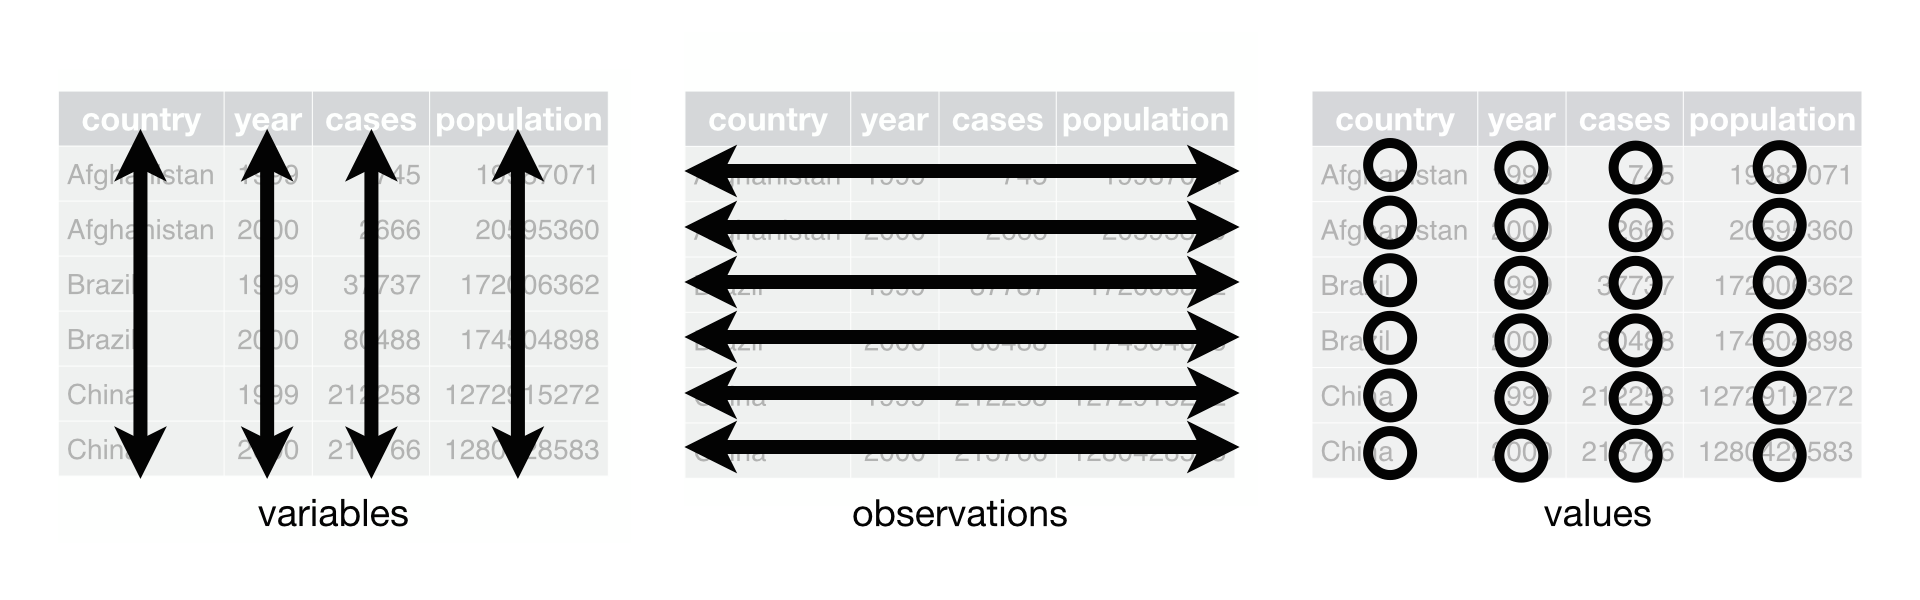
\includegraphics[width=\textwidth]{images/tidy-1} 

}

\caption[Tidy data graphic from http://r4ds.had.co.nz/tidy-data.html]{Tidy data graphic from http://r4ds.had.co.nz/tidy-data.html}\label{fig:tidyfig}
\end{figure}

Reading over this definition, you can begin to think about datasets that
won't follow this nice format.

\begin{center}\rule{0.5\linewidth}{\linethickness}\end{center}

\begin{learncheck}
\textbf{\emph{Learning check}}
\end{learncheck}

\textbf{(LC3.1)} Give an example dataset that doesn't follow this
format.

\begin{itemize}
\tightlist
\item
  What features of this dataset might make it difficult to visualize?\\
\item
  How could the dataset be tweaked to make it \textbf{tidy}?
\end{itemize}

\begin{center}\rule{0.5\linewidth}{\linethickness}\end{center}

\section{\texorpdfstring{The \texttt{nycflights13}
datasets}{The nycflights13 datasets}}\label{the-nycflights13-datasets}

We likely have all flown on airplanes or know someone that has. Air
travel has become an ever-present aspect of our daily lives. If you live
in or are visiting a relatively large city and you walk around that
city's airport, you see gates showing flight information from many
different airlines. And you will frequently see that some flights are
delayed because of a variety of conditions. Are there ways that we can
avoid having to deal with these flight delays?

We'd all like to arrive at our destinations on time whenever possible.
(Unless you secretly love hanging out at airports. If you are one of
these people, pretend for the moment that you are very much anticipating
being at your final destination.) Hadley Wickham (herein just referred
to as ``Hadley'') created multiple datasets containing information about
departing flights from the New York City area in 2013
\citep{R-nycflights13}. We will begin by loading in one of these
datasets, the \texttt{flights} dataset, and getting an idea of its
structure:

\begin{Shaded}
\begin{Highlighting}[]
\KeywordTok{library}\NormalTok{(nycflights13)}
\KeywordTok{data}\NormalTok{(flights)}
\end{Highlighting}
\end{Shaded}

The \texttt{library} function here loads the R package
\texttt{nycflights13} into the current R environment in which you are
working. (Note that you'll get an error if you try to load this package
in and it hasn't been installed. Check Chapter \ref{intro} to make sure
the package has been downloaded.) The next line of code
\texttt{data(flights)} loads in the \texttt{flights} dataset that is
stored in the \texttt{nycflights13} package.

This dataset and most others presented in this book will be in the
\texttt{data.frame} format in R. Dataframes are ways to look at
collections of variables that are tightly coupled together. Frequently,
the best way to get a feel for a dataframe is to use the \texttt{View}
function in RStudio. This command will be given throughout the book as a
reminder, but the actual output will be hidden.

\begin{Shaded}
\begin{Highlighting}[]
\KeywordTok{View}\NormalTok{(flights)}
\end{Highlighting}
\end{Shaded}

\begin{center}\rule{0.5\linewidth}{\linethickness}\end{center}

\begin{learncheck}
\textbf{\emph{Learning check}}
\end{learncheck}

\textbf{(LC3.4)} What does any \emph{ONE} row in this dataset refer to?

\begin{itemize}
\tightlist
\item
  A. Data on an airline
\item
  B. Data on a flight
\item
  C. Data on an airport
\item
  D. Data on multiple flights
\end{itemize}

\begin{center}\rule{0.5\linewidth}{\linethickness}\end{center}

By running \texttt{View(flights)}, we see the different
\textbf{variables} listed in the columns and we see that there are
different types of variables. Some of the variables like
\texttt{distance}, \texttt{day}, and \texttt{arr\_delay} are what we
will call \textbf{quantitative} variables. These variables vary in a
numerical way. Other variables here are \textbf{categorical}.

Note that if you look in the leftmost column of the
\texttt{View(flights)} output, you will see a column of numbers. These
are the row numbers of the dataset. If you glance across a row with the
same number, say row 5, you can get an idea of what each row correspond
to. In other words, this will allow you to identify what object is being
referred to in a given row. This is often called the
\textbf{observational unit}. The \textbf{observational unit} in this
example is an individual flight departing New York City in 2013.

\textbf{Note}: Frequently the first thing you should do when given a
dataset is to

\begin{itemize}
\tightlist
\item
  identify the observation unit,
\item
  specify the variables, and
\item
  give the types of variables you are presented with.
\end{itemize}

\begin{Shaded}
\begin{Highlighting}[]
\KeywordTok{str}\NormalTok{(flights)}
\end{Highlighting}
\end{Shaded}

\begin{verbatim}
## Classes 'tbl_df', 'tbl' and 'data.frame':    336776 obs. of  19 variables:
##  $ year          : int  2013 2013 2013 2013 2013 2013 2013 2013 2013 2013 ...
##  $ month         : int  1 1 1 1 1 1 1 1 1 1 ...
##  $ day           : int  1 1 1 1 1 1 1 1 1 1 ...
##  $ dep_time      : int  517 533 542 544 554 554 555 557 557 558 ...
##  $ sched_dep_time: int  515 529 540 545 600 558 600 600 600 600 ...
##  $ dep_delay     : num  2 4 2 -1 -6 -4 -5 -3 -3 -2 ...
##  $ arr_time      : int  830 850 923 1004 812 740 913 709 838 753 ...
##  $ sched_arr_time: int  819 830 850 1022 837 728 854 723 846 745 ...
##  $ arr_delay     : num  11 20 33 -18 -25 12 19 -14 -8 8 ...
##  $ carrier       : chr  "UA" "UA" "AA" "B6" ...
##  $ flight        : int  1545 1714 1141 725 461 1696 507 5708 79 301 ...
##  $ tailnum       : chr  "N14228" "N24211" "N619AA" "N804JB" ...
##  $ origin        : chr  "EWR" "LGA" "JFK" "JFK" ...
##  $ dest          : chr  "IAH" "IAH" "MIA" "BQN" ...
##  $ air_time      : num  227 227 160 183 116 150 158 53 140 138 ...
##  $ distance      : num  1400 1416 1089 1576 762 ...
##  $ hour          : num  5 5 5 5 6 5 6 6 6 6 ...
##  $ minute        : num  15 29 40 45 0 58 0 0 0 0 ...
##  $ time_hour     : POSIXct, format: "2013-01-01 05:00:00" ...
\end{verbatim}

\begin{center}\rule{0.5\linewidth}{\linethickness}\end{center}

\begin{learncheck}
\textbf{\emph{Learning check}}
\end{learncheck}

\textbf{(LC3.5)} What are some examples in this dataset of
\textbf{categorical} variables? What makes them different than
\textbf{quantitative} variables?

\textbf{(LC3.6)} What does \texttt{int}, \texttt{num}, and \texttt{chr}
mean in the output above?

\textbf{(LC3.7)} How many different columns are in this dataset?

\textbf{(LC3.8)} How many different rows are in this dataset?

\begin{center}\rule{0.5\linewidth}{\linethickness}\end{center}

Another way to view the properties of a dataset is to use the
\texttt{str} function (``str'' is short for ``structure''). This will
give you the first few entries of each variable in a row after the
variable. In addition, the type of the variable is given immediately
after the \texttt{:} following each variable's name. Here, \texttt{int}
and \texttt{num} refer to quantitative variables. In contrast,
\texttt{chr} refers to categorical variables. One more type of variable
is given here with the \texttt{time\_hour} variable: \textbf{POSIXct}.
As you may suspect, this variable corresponds to a specific date and
time of day.

Another nice feature of R is the help system. You can get help in R by
simply entering a question mark before the name of a function or an
object and you will be presented with a page showing the documentation.
Note that this output help file is omitted here but can be accessed
\href{https://cran.r-project.org/web/packages/nycflights13/nycflights13.pdf}{here}
on page 3 of the PDF document.

\begin{Shaded}
\begin{Highlighting}[]
\NormalTok{?flights}
\end{Highlighting}
\end{Shaded}

Another aspect of tidy data is a description of what each variable in
the dataset represents. This helps others to understand what your
variable names mean and what they correspond to. If we look at the
output of \texttt{?flights}, we can see that a description of each
variable by name is given.

An important feature to \textbf{ALWAYS} include with your data is the
appropriate units of measurement. We'll see this further when we work
with the \texttt{dep\_delay} variable in Chapter \ref{viz}. (It's in
minutes, but you'd get some really strange interpretations if you
thought it was in hours or seconds. UNITS MATTER!)

\section{\texorpdfstring{How is \texttt{flights}
tidy?}{How is flights tidy?}}\label{how-is-flights-tidy}

We see that \texttt{flights} has a rectangular shape with each row
corresponding to a different flight and each column corresponding to a
characteristic of that flight. This matches exactly with how Hadley
defined tidy data:

\begin{enumerate}
\def\labelenumi{\arabic{enumi}.}
\tightlist
\item
  Each variable forms a column.
\item
  Each observation forms a row.
\end{enumerate}

But what about the third property?

\begin{quote}
\begin{enumerate}
\def\labelenumi{\arabic{enumi}.}
\setcounter{enumi}{2}
\tightlist
\item
  Each type of observational unit forms a table.
\end{enumerate}
\end{quote}

We identified earlier that the observational unit in the
\texttt{flights} dataset is an individual flight. And we have shown that
this dataset consists of 336,776 flights with 19 variables. In other
words, some rows of this dataset don't refer to a measurement on an
airline or on an airport. They specifically refer to
characteristics/measurements on a given \textbf{flight} from New York
City in 2013.

By contrast, also included in the \texttt{nycflights13} package are
datasets with different observational units \citep{R-nycflights13}:

\begin{itemize}
\tightlist
\item
  \texttt{weather}: hourly meteorological data for each airport
\item
  \texttt{planes}: construction information about each plane
\item
  \texttt{airports}: airport names and locations
\item
  \texttt{airlines}: translation between two letter carrier codes and
  names
\end{itemize}

You may have been asking yourself what \texttt{carrier} refers to in the
\texttt{str(flights)} output above. The \texttt{airlines} dataset
provides a description of this with each airline being the observational
unit:

\begin{Shaded}
\begin{Highlighting}[]
\KeywordTok{data}\NormalTok{(airlines)}
\NormalTok{airlines}
\end{Highlighting}
\end{Shaded}

\begin{verbatim}
##    carrier                        name
## 1       9E           Endeavor Air Inc.
## 2       AA      American Airlines Inc.
## 3       AS        Alaska Airlines Inc.
## 4       B6             JetBlue Airways
## 5       DL        Delta Air Lines Inc.
## 6       EV    ExpressJet Airlines Inc.
## 7       F9      Frontier Airlines Inc.
## 8       FL AirTran Airways Corporation
## 9       HA      Hawaiian Airlines Inc.
## 10      MQ                   Envoy Air
## 11      OO       SkyWest Airlines Inc.
## 12      UA       United Air Lines Inc.
## 13      US             US Airways Inc.
## 14      VX              Virgin America
## 15      WN      Southwest Airlines Co.
## 16      YV          Mesa Airlines Inc.
\end{verbatim}

As can be seen here when you just enter the name of an object in R, by
default it will print the contents of that object to the screen. Be
careful! It's usually better to use the \texttt{View()} function in
RStudio since larger objects may take awhile to print to the screen and
it likely won't be helpful to you to have hundreds of lines outputted.

\section{Normal forms of data}\label{normal-forms-of-data}

The datasets included in the \texttt{nycflights13} package are in a form
that minimizes redundancy of data. We will see that there are ways to
\emph{merge} (or \emph{join}) the different tables together easily. We
are capable of doing so because each of the tables have \emph{keys} in
common to relate one to another. This is an important property of
\textbf{normal forms} of data. The process of decomposing dataframes
into less redundant tables without losing information is called
\textbf{normalization}. More information is available on
\href{https://en.wikipedia.org/wiki/Database_normalization}{Wikipedia}.

We saw an example of this above with the \texttt{airlines} dataset.
While the \texttt{flights} dataframe could also include a column with
the names of the airlines instead of the carrier code, this would be
repetitive since there is a unique mapping of the carrier code to the
name of the airline/carrier.

Below an example is given showing how to \textbf{join} the
\texttt{airlines} dataframe together with the \texttt{flights} dataframe
by linking together the two datasets via a common \textbf{key} of
\texttt{"carrier"}. Note that this ``joined'' dataframe is assigned to a
new dataframe called \texttt{joined\_flights}.

\begin{Shaded}
\begin{Highlighting}[]
\KeywordTok{library}\NormalTok{(dplyr)}
\NormalTok{joined_flights <-}\StringTok{ }\KeywordTok{inner_join}\NormalTok{(}\DataTypeTok{x =} \NormalTok{flights, }\DataTypeTok{y =} \NormalTok{airlines, }\DataTypeTok{by =} \StringTok{"carrier"}\NormalTok{)}
\end{Highlighting}
\end{Shaded}

\begin{Shaded}
\begin{Highlighting}[]
\KeywordTok{View}\NormalTok{(joined_flights)}
\end{Highlighting}
\end{Shaded}

If we \texttt{View} this dataset, we see a new variable has been created
called (We will see in Subsection 5.1.1 ways to change \texttt{name} to
a more descriptive variable name.)

More discussion about joining dataframes together will be given in
Chapter \ref{manip}. We will see there that the names of the columns to
be linked need not match as they did here with \texttt{"carrier"}.

\begin{center}\rule{0.5\linewidth}{\linethickness}\end{center}

\begin{center}\rule{0.5\linewidth}{\linethickness}\end{center}

\begin{review}
\textbf{\emph{Review questions}}
\end{review}

\textbf{(RQ3.1)} What are common characteristics of ``tidy'' datasets?

\textbf{(RQ3.2)} What makes ``tidy'' datasets useful for organizing
data?

\textbf{(RQ3.4)} How many variables are presented in the table below?
What does each row correspond to? (\textbf{Hint:} You may not be able to
answer both of these questions immediately but take your best guess.)

\begin{tabular}{r|r}
\hline
students & faculty\\
\hline
4 & 2\\
\hline
6 & 3\\
\hline
\end{tabular}

\textbf{(RQ3.5)} The confusion you may have encountered in Question 4 is
a common one those that work with data are commonly presented with. This
dataset is not tidy. Actually, the dataset in Question 4 has three
variables not the two that were presented. Make a guess as to what these
variables are and present a tidy dataset instead of this untidy one
given in Question 4.

\textbf{(RQ3.6)} The actual data presented in Question 4 is given below
in tidy data format:

\begin{tabular}{l|l|l}
\hline
role & Sociology? & Type of School\\
\hline
student & TRUE & Public\\
\hline
student & TRUE & Public\\
\hline
student & TRUE & Public\\
\hline
student & TRUE & Public\\
\hline
student & FALSE & Public\\
\hline
student & FALSE & Public\\
\hline
student & FALSE & Private\\
\hline
student & FALSE & Private\\
\hline
student & FALSE & Private\\
\hline
student & FALSE & Private\\
\hline
faculty & TRUE & Public\\
\hline
faculty & TRUE & Public\\
\hline
faculty & FALSE & Public\\
\hline
faculty & FALSE & Private\\
\hline
faculty & FALSE & Private\\
\hline
\end{tabular}

\begin{itemize}
\tightlist
\item
  What does each row correspond to?\\
\item
  What are the different variables in this dataframe?\\
\item
  The \texttt{Sociology?} variable is known as a logical variable. What
  types of values does a logical variable take on?
\end{itemize}

\textbf{(RQ3.7)} What are some advantages of data in normal forms? What
are some disadvantages?

\begin{center}\rule{0.5\linewidth}{\linethickness}\end{center}

\begin{center}\rule{0.5\linewidth}{\linethickness}\end{center}

\section{What's to come?}\label{whats-to-come}

In Chapter \ref{viz}, we will further explore the distribution of a
variable in a related dataset to \texttt{flights}: the \texttt{temp}
variable in the \texttt{weather} dataset. We'll be interested in
understanding how this variable varies in relation to the values of
other variables in the dataset. We will see that visualization is often
a powerful tool in helping us see what is going on in a dataset. It will
be a useful way to expand on the \texttt{str} function we have seen here
for tidy data.

\chapter{Visualizing Data}\label{viz}

In Chapter \ref{tidy}, we discussed the importance of datasets being
\textbf{tidy}. You will see in examples here why having a tidy dataset
helps us immensely with plotting our data. In plotting our data, we will
be able to gain valuable insights from our data that we couldn't
initially see from just looking at the raw tidy data. We will focus on
using Hadley's \texttt{ggplot2} package in doing so, which was developed
to work specifically on datasets that are \textbf{tidy}. It provides an
easy way to customize your plots and is based on data visualization
theory given in \emph{The Grammar of Graphics} \citep{wilkinson2005}.

Graphics provide a nice way for us to get a sense for how quantitative
variables compare in terms of their center and their spread. The most
important thing to know about graphics is that they should be created to
make it obvious for your audience to see the findings you want to get
across. This requires a balance on not including too much in your plots,
but also including enough so that relationships and interesting findings
can be easily seen. As we will see, plots/graphics also help us to
identify patterns and outliers in our data. We will see that a common
extension of these ideas is to compare the distribution (i.e., what the
spread of a variable looks like) as we go across the levels of a
different categorical variable.

\section{Five Named Graphs - The FNG}\label{five-named-graphs---the-fng}

For our purposes here, we will be working with five different types of
graphs. (Note that we will use a lot of different words here in regards
to plotting - ``graphs'', ``plots'', and ``charts'' are all ways to
discuss a resulting graphic. You can think of them as all being
synonyms.) These five plots are:

\begin{itemize}
\tightlist
\item
  histograms
\item
  boxplots
\item
  barplots
\item
  scatter-plots
\item
  line-graphs
\end{itemize}

With this toolbox of plots, you can visualize just about any type of
variable thrown at you. We will discuss some other variations of these
but with the FNG in your repertoire you can do big things! Something we
will also stress here is that certain plots only work for
categorical/logical variables and others only for quantitative
variables. You'll want to quiz yourself often on which plot makes sense
with a given problem set-up.

We now introduce another dataframe in the \texttt{nycflights13} package
introduced in Chapter \ref{tidy}.

\begin{Shaded}
\begin{Highlighting}[]
\KeywordTok{library}\NormalTok{(nycflights13)}
\KeywordTok{data}\NormalTok{(weather)}
\end{Highlighting}
\end{Shaded}

\section{Histograms}\label{histograms}

Our focus now turns to the \texttt{temp} variable in this
\texttt{weather} dataset. We would like to visualize what the 26130
temperatures look like. Looking over the \texttt{weather}
dataset\footnote{Recall that to view a dataset in spreadsheet format in
  RStudio, you can run the \texttt{View()} function with the dataframe
  as its argument.} and running \texttt{?weather}, we can see that the
\texttt{temp} variable corresponds to hourly temperature (in Fahrenheit)
recordings at weather stations near airports in New York City. We could
just produce points where each of the different values appears on
something similar to a number line:

\begin{figure}

{\centering 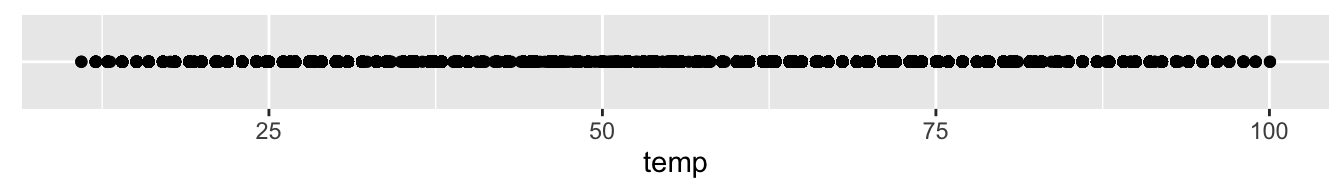
\includegraphics[width=\textwidth]{ismay_files/figure-latex/unnamed-chunk-14-1} 

}

\caption[Strip Plot of Hourly Temperature Recordings from NYC in 2013]{Strip Plot of Hourly Temperature Recordings from NYC in 2013}\label{fig:unnamed-chunk-14}
\end{figure}

This gives us a general idea of how the values of \texttt{temp} differ.
We see that temperatures vary from around 11 up to 100 degrees
Fahrenheit. The area between 40 and 60 degrees appears to have more
points plotted than outside that range.

What is commonly produced instead of this strip plot is a plot known as
a \textbf{histogram}. The \textbf{histogram} show how many elements of
the variable fall in specified \textbf{bins}. These \textbf{bins} may
correspond to between 0-10°F, 10-20°F, etc.

To produce a histogram, we introduce the Hadley's \texttt{ggplot2}
package \citep{R-ggplot2}. We will use the \texttt{ggplot} function
which expects at a bare minimal as arguments

\begin{itemize}
\tightlist
\item
  the dataframe where the variables exist and
\item
  the names of the variables to be plotted.
\end{itemize}

The names of the variables will be entered into the \texttt{aes}
function as arguments where \texttt{aes} stands for ``aesthetics''.

\begin{Shaded}
\begin{Highlighting}[]
\KeywordTok{ggplot}\NormalTok{(}\DataTypeTok{data =} \NormalTok{weather, }\DataTypeTok{mapping =} \KeywordTok{aes}\NormalTok{(}\DataTypeTok{x =} \NormalTok{temp))}
\end{Highlighting}
\end{Shaded}

\begin{figure}

{\centering 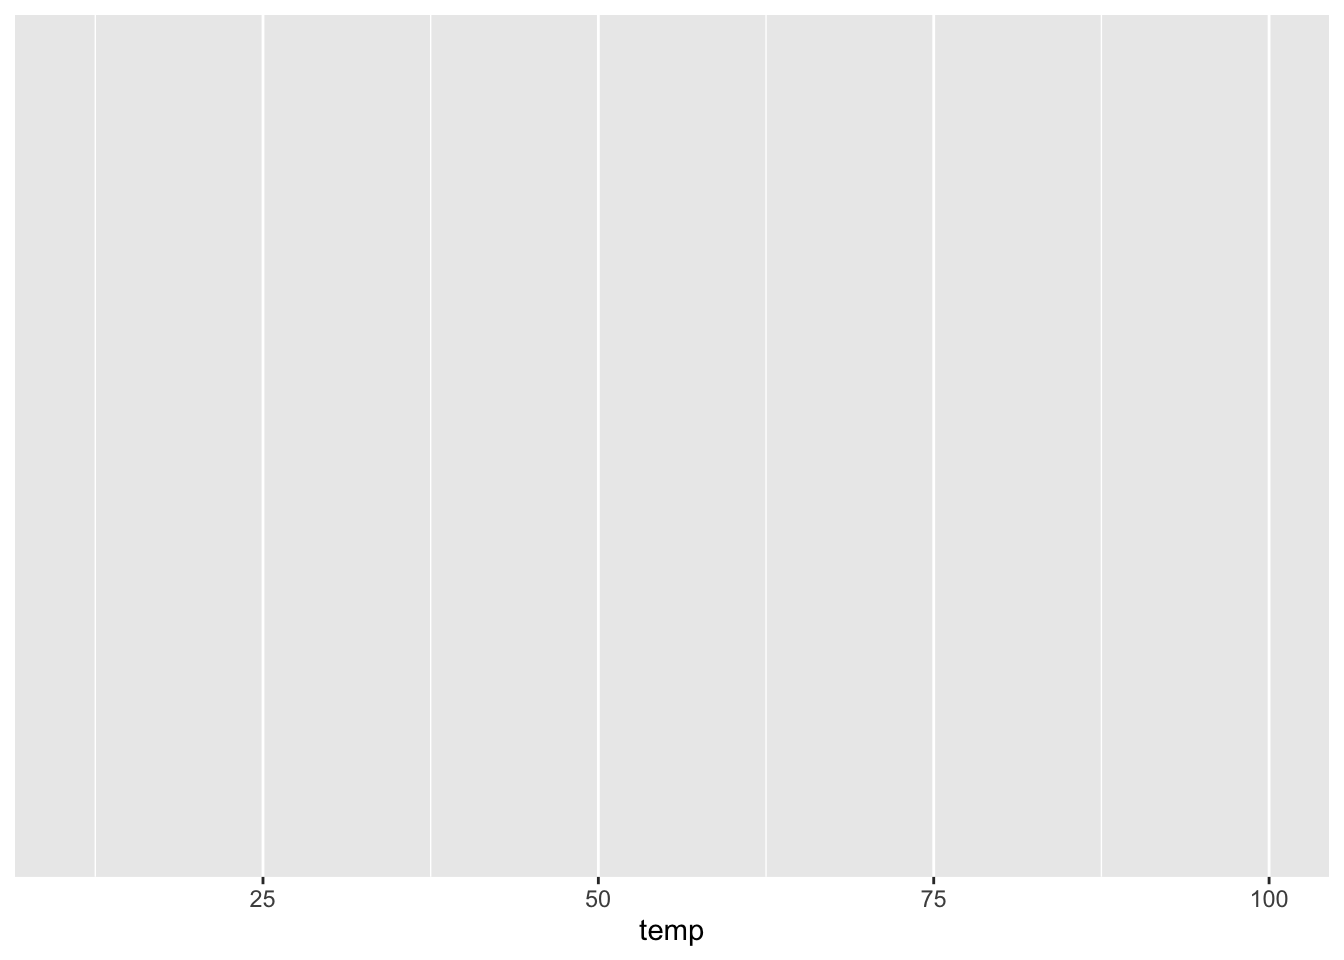
\includegraphics[width=\textwidth]{ismay_files/figure-latex/unnamed-chunk-15-1} 

}

\caption[ggplot backdrop]{ggplot backdrop}\label{fig:unnamed-chunk-15}
\end{figure}

The plot given above is not a histogram, but the output does show us a
bit of what is going on with
\texttt{ggplot(data\ =\ weather,\ mapping\ =\ aes(x\ =\ temp))}. It is
producing a backdrop onto which we will ``paint'' elements.

We next proceed by adding a layer---hence, the use of the \texttt{+}
symbol---to the plot to produce a histogram. (Note also here that we
don't have to specify the \texttt{data\ =} and \texttt{mapping\ =} text
in our function calls. This is covered in more detail in Chapter 5 of
the ``Getting Used to R, RStudio, and R Markdown'' book
\citep{usedtor2016}).

\begin{Shaded}
\begin{Highlighting}[]
\KeywordTok{ggplot}\NormalTok{(}\DataTypeTok{data =} \NormalTok{weather, }\DataTypeTok{mapping =} \KeywordTok{aes}\NormalTok{(}\DataTypeTok{x =} \NormalTok{temp)) +}
\StringTok{  }\KeywordTok{geom_histogram}\NormalTok{()}
\end{Highlighting}
\end{Shaded}

\begin{verbatim}
## `stat_bin()` using `bins = 30`. Pick better value with `binwidth`.
\end{verbatim}

\begin{verbatim}
## Warning: Removed 1 rows containing non-finite values (stat_bin).
\end{verbatim}

\begin{figure}

{\centering 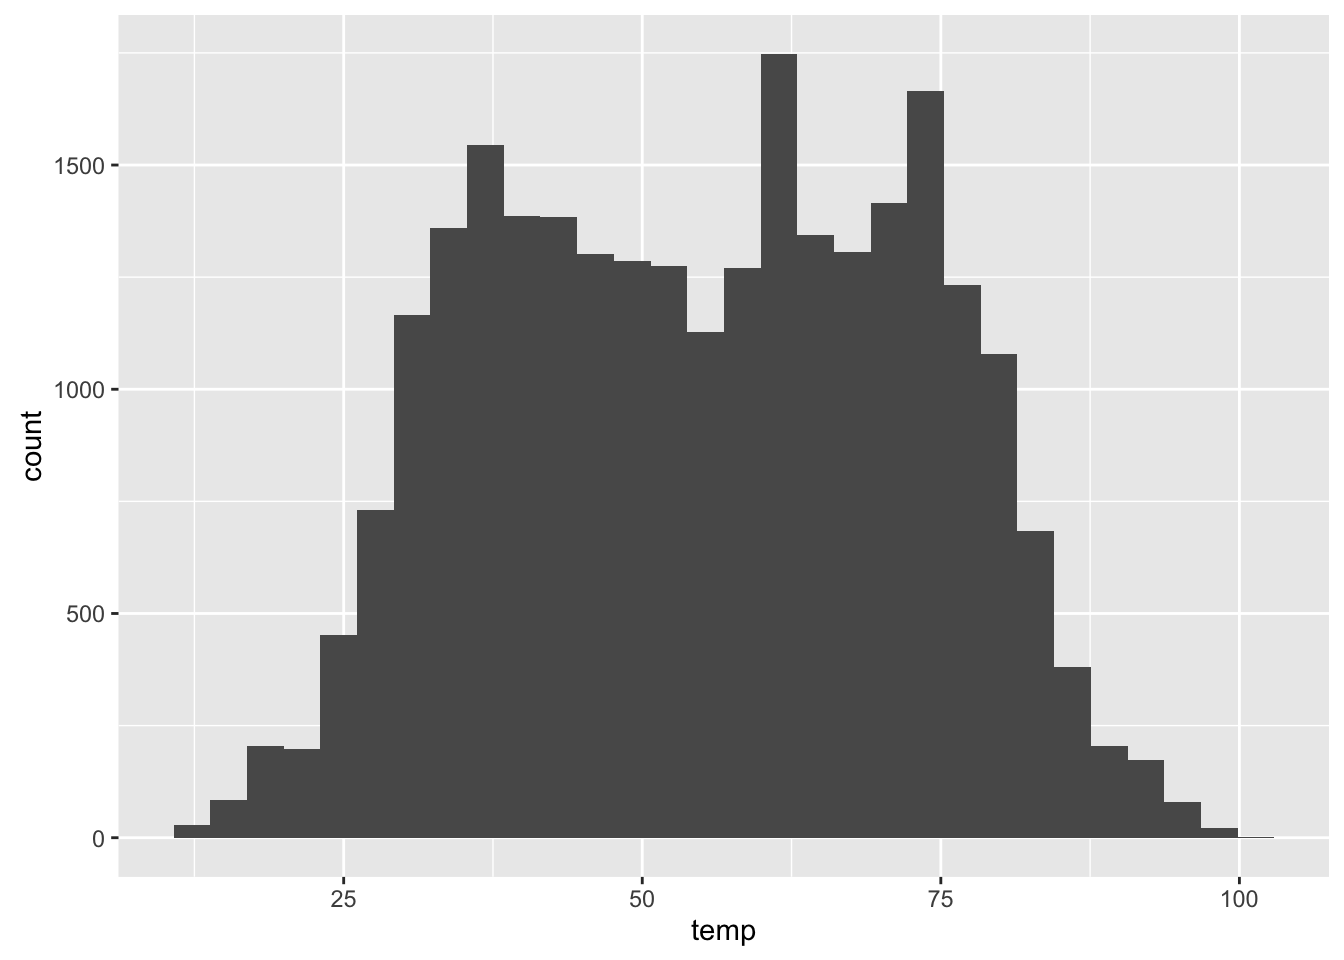
\includegraphics[width=\textwidth]{ismay_files/figure-latex/unnamed-chunk-16-1} 

}

\caption[Histogram of Hourly Temperature Recordings from NYC in 2013]{Histogram of Hourly Temperature Recordings from NYC in 2013}\label{fig:unnamed-chunk-16}
\end{figure}

We have the power to specify how many bins we would like to put the data
into as an argument in the \texttt{geom\_histogram} function. By
default, this is chosen to be 30 somewhat arbitrarily and we have
received a warning above our plot that this was done. We also notice
here that another warning about 1 missing value is given. This value is
omitted from the plot. This warning is ignored for future customizations
of the plot.

Missing values are a common problem when working with data and there are
entire fields of study on how to work with missing data. Frequently what
is done is to remove instances from the data set that are missing. This
is certainly the easy way to deal with them, but not necessarily the
correct decision in all cases. For our purposes, we will usually ignore
potential warnings about missing data since R can usually handle them by
ignoring them.

\begin{Shaded}
\begin{Highlighting}[]
\KeywordTok{ggplot}\NormalTok{(}\DataTypeTok{data =} \NormalTok{weather, }\DataTypeTok{mapping =} \KeywordTok{aes}\NormalTok{(}\DataTypeTok{x =} \NormalTok{temp)) +}
\StringTok{  }\KeywordTok{geom_histogram}\NormalTok{(}\DataTypeTok{bins =} \DecValTok{60}\NormalTok{)}
\end{Highlighting}
\end{Shaded}

\begin{figure}

{\centering 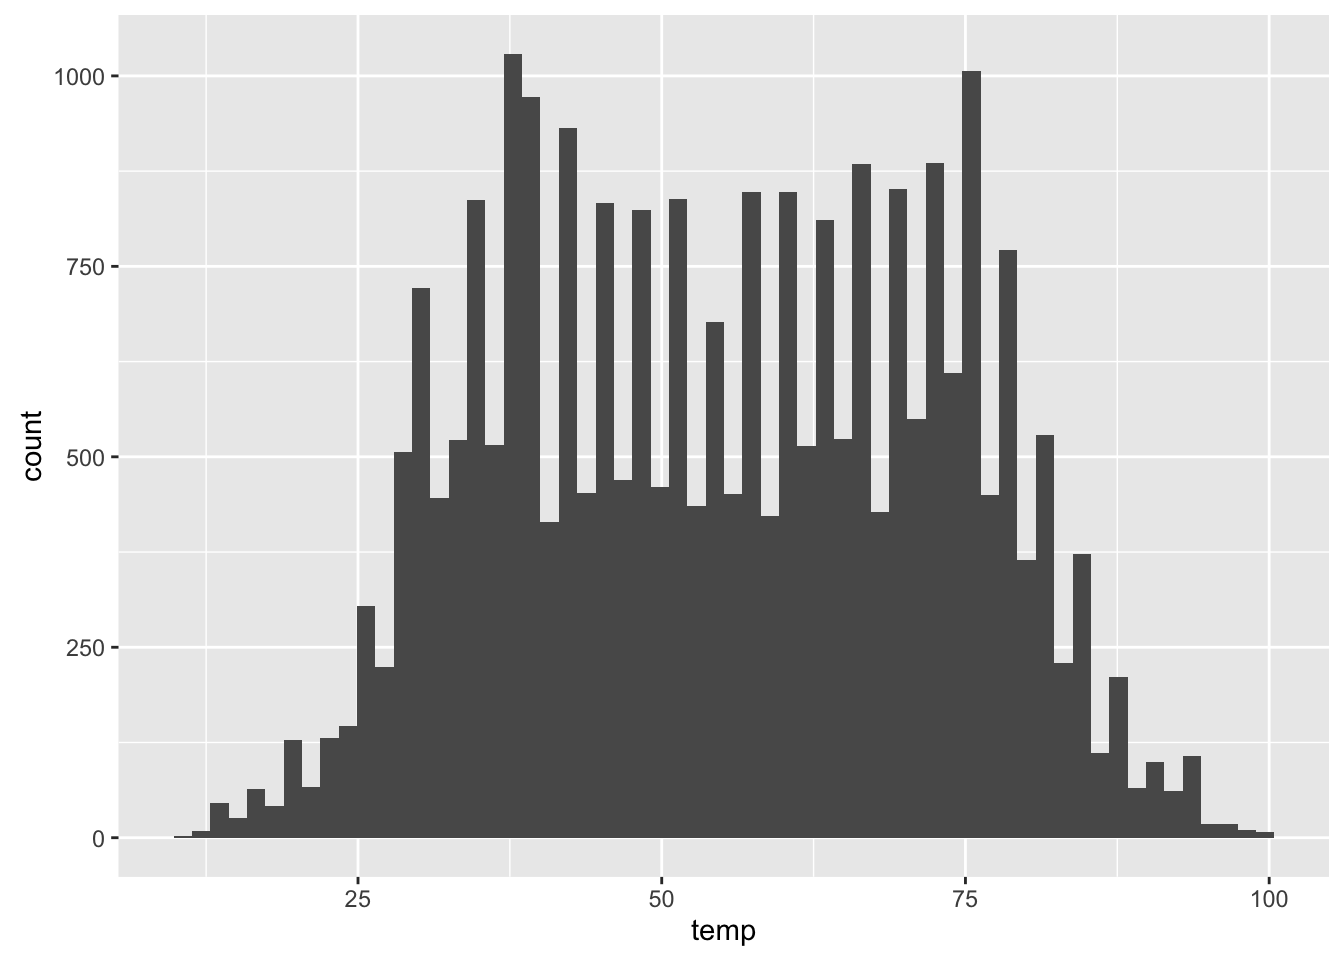
\includegraphics[width=\textwidth]{ismay_files/figure-latex/unnamed-chunk-17-1} 

}

\caption[Histogram of Hourly Temperature Recordings from NYC in 2013 - 60 Bins]{Histogram of Hourly Temperature Recordings from NYC in 2013 - 60 Bins}\label{fig:unnamed-chunk-17}
\end{figure}

We can tweak the plot a little more by specifying the width of the bins
(instead of how many bins to divide the variable into) by using the
\texttt{binwidth} argument in the \texttt{geom\_histogram} function. We
can also add some color to the plot by invoking the \texttt{fill} and
\texttt{color} arguments. A listing of all of the built-in colors to R
by name and color is available
\href{http://www.stat.columbia.edu/~tzheng/files/Rcolor.pdf}{here}.

\begin{Shaded}
\begin{Highlighting}[]
\KeywordTok{ggplot}\NormalTok{(}\DataTypeTok{data =} \NormalTok{weather, }\DataTypeTok{mapping =} \KeywordTok{aes}\NormalTok{(}\DataTypeTok{x =} \NormalTok{temp)) +}
\StringTok{  }\KeywordTok{geom_histogram}\NormalTok{(}\DataTypeTok{binwidth =} \DecValTok{10}\NormalTok{, }\DataTypeTok{color =} \StringTok{"white"}\NormalTok{, }\DataTypeTok{fill =} \StringTok{"forestgreen"}\NormalTok{)}
\end{Highlighting}
\end{Shaded}

\begin{figure}

{\centering 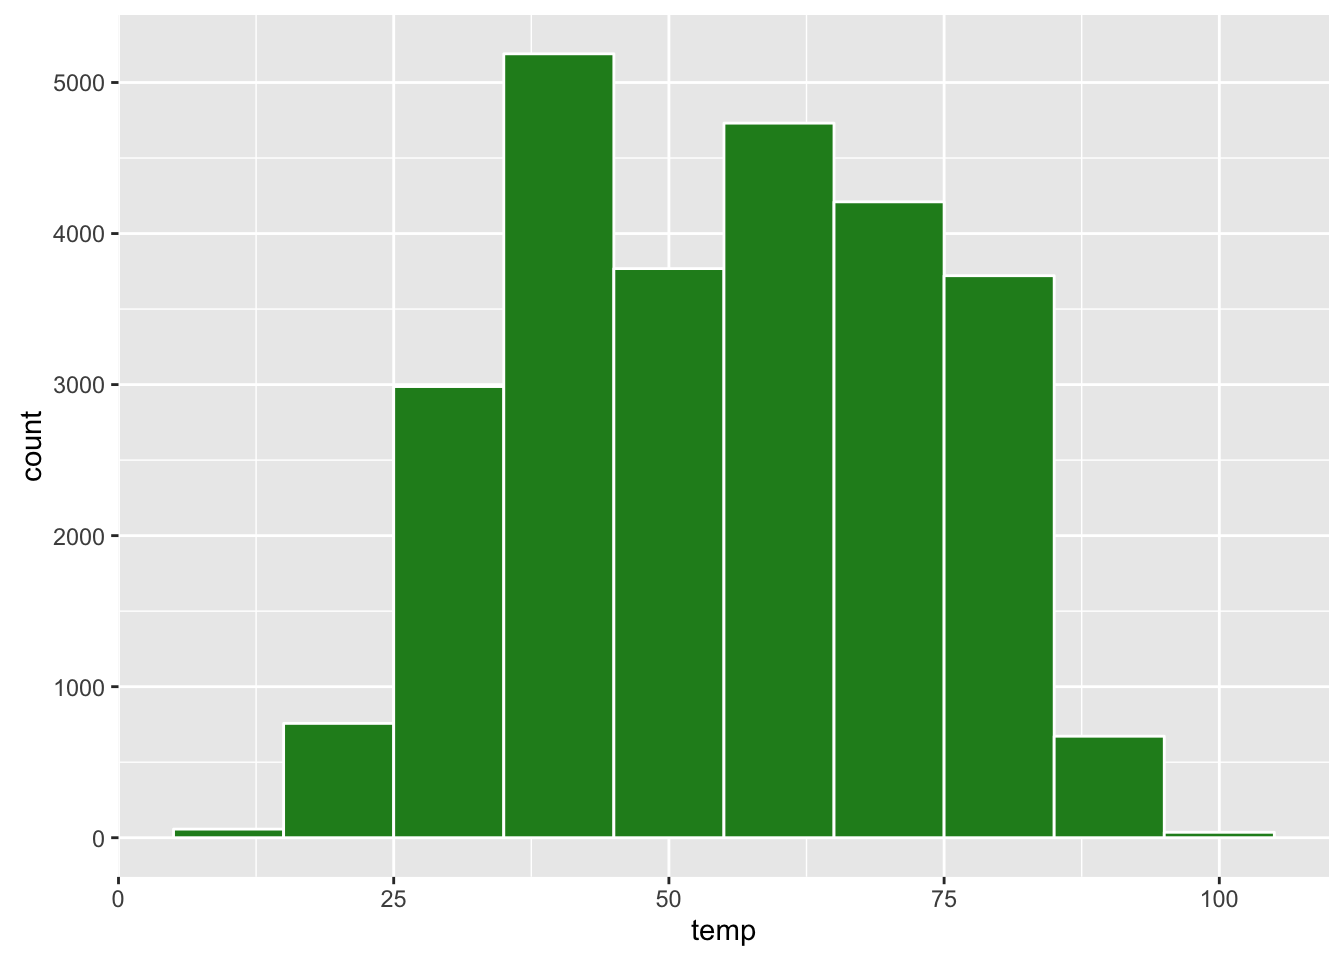
\includegraphics[width=\textwidth]{ismay_files/figure-latex/unnamed-chunk-18-1} 

}

\caption[Histogram of Hourly Temperature Recordings from NYC in 2013 - Binwidth = 10]{Histogram of Hourly Temperature Recordings from NYC in 2013 - Binwidth = 10}\label{fig:unnamed-chunk-18}
\end{figure}

\begin{center}\rule{0.5\linewidth}{\linethickness}\end{center}

\begin{learncheck}
\textbf{\emph{Learning check}}
\end{learncheck}

\textbf{(LC4.1)} What does changing the number of bins from 30 to 60
tell us about the distribution of temperatures?

\textbf{(LC4.2)} Would you classify the distribution of temperatures as
symmetric or skewed?

\textbf{(LC4.3)} What would you guess is the ``center'' value in this
distribution? Why did you make that choice?

\textbf{(LC4.4)} Is this data spread out greatly from the center or is
it close? Why?

\begin{center}\rule{0.5\linewidth}{\linethickness}\end{center}

\subsection{Continuous data summaries}\label{contsum}

The \texttt{temp} variable is a \textbf{continuous} quantitative
variable (frequently just called a \textbf{continuous variable}). ``A
variable is \textbf{continuous} if you can arrange its values in order
and an infinite number of unique values can exist between any two values
of the variable''\citep{rds2016}. Some common examples of continuous
variables are time and height. Between any two times there are an
infinitely many number of time units that fall between them.

It is often easier to think about quantitative variables that are not
continuous to help us better understand continuity. The best example is
counts. If we are looking to count the number of flights that depart on
a given day from New York City, this variable would not be continuous.
It falls on a \textbf{discrete} scale.

We can examine some summary information about this \texttt{temp}
variable. To do so, we introduce the \texttt{summary} function. (We will
see in Chapter \ref{manip} how to use the \texttt{summarize} function in
the \texttt{dplyr} package to produce similar results.)

The syntax here is a little different than what we have seen before. (A
further discussion about R syntax is available in Chapter 5 of the ``R
basics'' book \citep{usedtor2016}). Here, \texttt{summary} is the
function and it is expecting an object to be summarized as its argument.
The object here is the \texttt{temp} variable in the \texttt{weather}
dataframe. To focus on just this one variable \texttt{temp} in
\texttt{weather}, we separate them by the dollar sign symbol
\texttt{\$}. Order matters here: the dataframe comes before the
\texttt{\$} and the variable/column name comes after.

\begin{Shaded}
\begin{Highlighting}[]
\KeywordTok{summary}\NormalTok{(weather$temp)}
\end{Highlighting}
\end{Shaded}

\begin{verbatim}
##    Min. 1st Qu.  Median    Mean 3rd Qu.    Max.    NA's 
##   10.94   39.92   55.04   55.20   69.98  100.00       1
\end{verbatim}

This tells us what is known as the \textbf{five-number summary} for our
variable as well as the \textbf{mean} value of the variable. More
information on both of these concepts is given in Appendix B - Chapter
\ref{appendix2}.

This \texttt{summary} gives us some numerical summaries of our
temperature variable. The minimum recorded temperature is 10.94 degrees
Fahrenheit and the maximum is 100.04 degrees Fahrenheit. We have one
missing value denoted as an \texttt{NA} in the observations of this
variable. The median Fahrenheit temperature of 55.04 and mean of
55.2035149 are quite close. This is a property of symmetric
distributions.

The last two entries given by \texttt{summary} correspond to the
25\textsuperscript{th} percentile and the 75\textsuperscript{th}
percentile. If we sorted all of the temperatures in increasing order, we
would see that 25\% of them would fall below 39.92 and that 75\% of them
would fall below 69.98. This implies that the middle 50\% of data values
lie between 39.92 and 69.98 degrees Fahrenheit.

Another common measure to determine the variability of a data set is the
\textbf{standard deviation}. You can read further about the mathematical
details of standard deviation in Appendix B - Chapter \ref{appendix2},
but you can think of it as being a measure of how far the data is, on
average, from the mean. Let's investigate this further by calculating
the standard deviation of our temperature variable:

\begin{Shaded}
\begin{Highlighting}[]
\KeywordTok{sd}\NormalTok{(weather$temp)}
\end{Highlighting}
\end{Shaded}

\begin{verbatim}
## [1] NA
\end{verbatim}

Remember that there were some missing values in our temperature data
when we plotted it earlier. By default, the \texttt{sd} function that
computes standard deviation of a variable will give the value of
\texttt{NA} if any of the data is missing. To further understand this,
you can look at the help of the \texttt{sd} function in the R Console:

\begin{Shaded}
\begin{Highlighting}[]
\NormalTok{?sd}
\end{Highlighting}
\end{Shaded}

Under \textbf{Usage} you can see that \texttt{na.rm} is set to
\texttt{FALSE} by default. We'd like for missing values to be removed
from our analysis so we set that value to \texttt{TRUE}:

\begin{Shaded}
\begin{Highlighting}[]
\KeywordTok{sd}\NormalTok{(weather$temp, }\DataTypeTok{na.rm =} \OtherTok{TRUE}\NormalTok{)}
\end{Highlighting}
\end{Shaded}

\begin{verbatim}
## [1] 17.78212
\end{verbatim}

Standard deviation is always in the same units as our original data set.
So in this case the standard deviation is in degrees Fahrenheit. Thus,
we can interpret this value saying:

For a randomly selected element in our temperature column, we can expect
it to be about 17.7821236 degrees Fahrenheit from our mean value of
`55.2035149. By combining this knowledge with the plots above, we can
have a good idea for whether this data is very spread out from its
center or if it is tightly bunched.

\subsection{Summary}\label{summary}

Histograms provide a useful way of looking at how ONE continuous
variable varies. They allow us to answer questions such as

\begin{itemize}
\tightlist
\item
  Are there values far away from the center? These are commonly called
  \textbf{outliers} and can frequently be easily identified on a
  histogram.
\item
  Are most values close to the center? If so, the spread of the variable
  is small. If not, the spread is large.
\item
  How spread out are the values? One measure of this spread is
  \textbf{standard deviation} discussed above.
\end{itemize}

The histogram shows how many entries fall in different groupings of this
variable. Another common property of distributions is symmetry and as we
saw it is quite easily identified by looking over the histogram produced
from the variable's values.

\section{Boxplots}\label{boxplots}

Histograms can also be produced to compare the distribution of a
variable over another variable. Suppose we were interested in looking at
how the temperature recordings we saw in the last section varied by
month. This is what is meant by ``the distribution of a variable over
another variable'': \texttt{temp} is one variable and \texttt{month} is
the other variable.

\subsection{Faceting}\label{faceting}

In order to look at histograms of \texttt{temp} for each month, we
introduce a new concept called \textbf{facetting}. Faceting is used when
we'd like to create small multiples of the same plot over a different
categorical variable. By default, all of the small multiples will have
the same vertical axis. An example will help here. We will discuss the
concept of faceting in further detail in Section \ref{barplots}.

\begin{Shaded}
\begin{Highlighting}[]
\KeywordTok{ggplot}\NormalTok{(}\DataTypeTok{data =} \NormalTok{weather, }\DataTypeTok{mapping =} \KeywordTok{aes}\NormalTok{(}\DataTypeTok{x =} \NormalTok{temp)) +}
\StringTok{  }\KeywordTok{geom_histogram}\NormalTok{(}\DataTypeTok{binwidth =} \DecValTok{5}\NormalTok{, }\DataTypeTok{color =} \StringTok{"white"}\NormalTok{, }\DataTypeTok{fill =} \StringTok{"firebrick"}\NormalTok{) +}
\StringTok{  }\KeywordTok{facet_wrap}\NormalTok{(~month)}
\end{Highlighting}
\end{Shaded}

\begin{figure}

{\centering 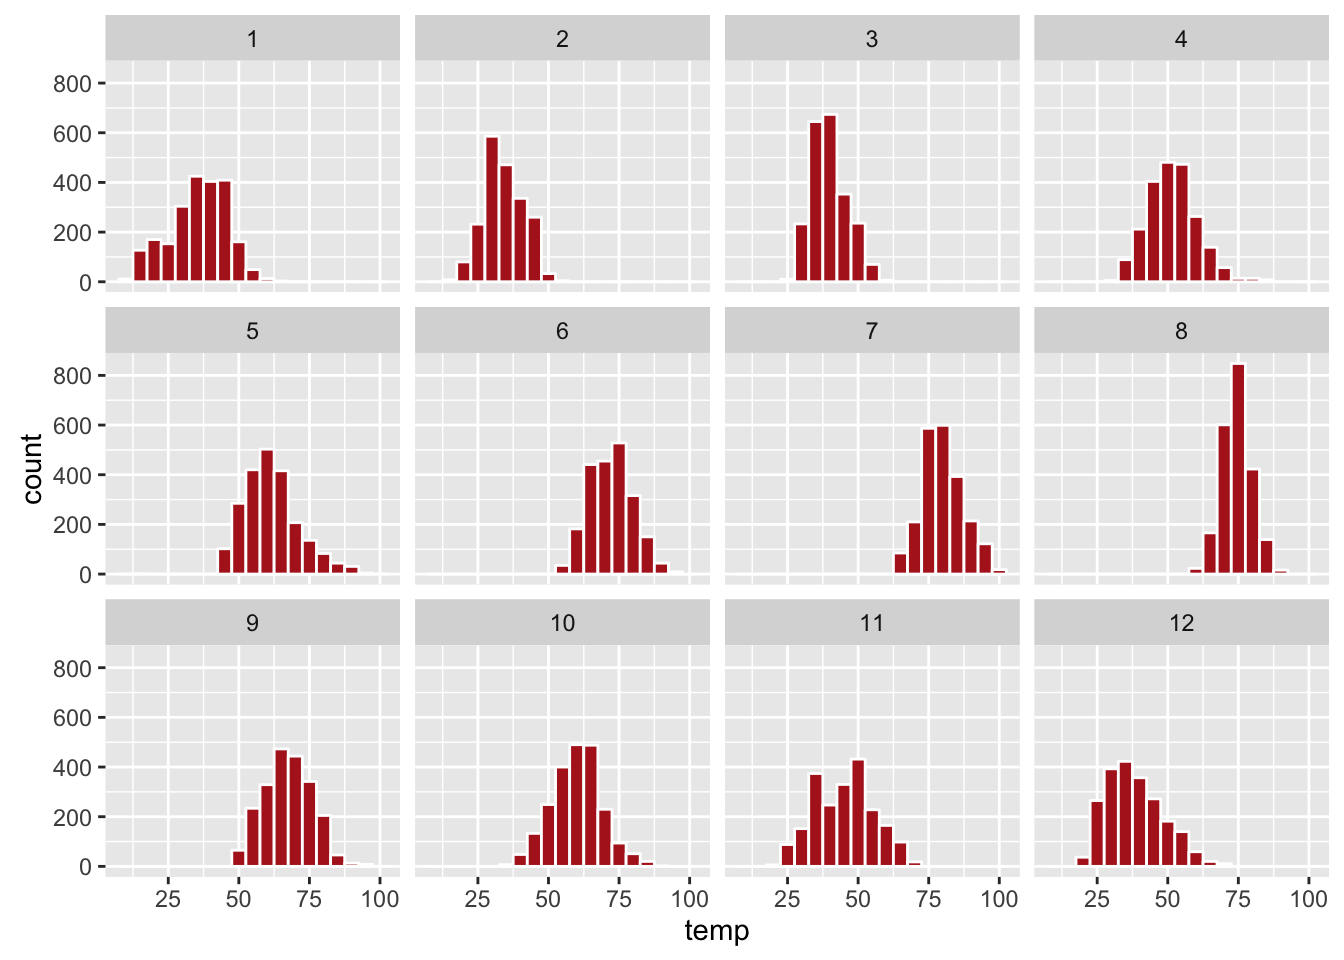
\includegraphics[width=\textwidth]{ismay_files/figure-latex/facethistogram-1} 

}

\caption[Faceted histogram]{Faceted histogram}\label{fig:facethistogram}
\end{figure}

As we might expect, the temperature tends to increase as summer
approaches and then decrease as winter approaches.

\begin{center}\rule{0.5\linewidth}{\linethickness}\end{center}

\begin{learncheck}
\textbf{\emph{Learning check}}
\end{learncheck}

\textbf{(LC4.5)} What other things do you notice about the faceted plot
above? How does a faceted plot help us see how relationships between two
variables?

\textbf{(LC4.6)} What do the numbers 1-12 correspond to in the plot
above? What about 25, 50, 75, 100?

\textbf{(LC4.7)} What could be done to make the faceted plot above more
readable? (Focus on tweaking the histograms and not on making a
different type of plot here.)

\textbf{(LC4.8)} For which types of datasets would these types of
faceted plots not work well in comparing relationships between
variables? Draw or give an example.

\textbf{(LC4.9)} Does the \texttt{temp} variable in the \texttt{weather}
data set have a lot of variability? Why do you say that?

\begin{center}\rule{0.5\linewidth}{\linethickness}\end{center}

Histograms can provide a way to compare distributions across groups as
we see above when we looked at temperature over months. Frequently, a
plot called a \textbf{boxplot} (also called a \textbf{side-by-side
boxplot}) is done instead. The \textbf{boxplot} uses the information
provided in the \textbf{five-number summary} referred to in the previous
section when we used the \texttt{summary} function. It gives a way to
compare this summary information across the different levels of a group.
Let's create a boxplot to compare the monthly temperatures as we did
above with the faceted histograms.

\begin{Shaded}
\begin{Highlighting}[]
\KeywordTok{ggplot}\NormalTok{(}\DataTypeTok{data =} \NormalTok{weather, }\DataTypeTok{mapping =} \KeywordTok{aes}\NormalTok{(}\DataTypeTok{x =} \NormalTok{month, }\DataTypeTok{y =} \NormalTok{temp)) +}
\StringTok{  }\KeywordTok{geom_boxplot}\NormalTok{()}
\end{Highlighting}
\end{Shaded}

\begin{verbatim}
## Warning: Continuous x aesthetic -- did you forget aes(group=...)?
\end{verbatim}

\begin{verbatim}
## Warning: Removed 1 rows containing non-finite values (stat_boxplot).
\end{verbatim}

\begin{figure}

{\centering 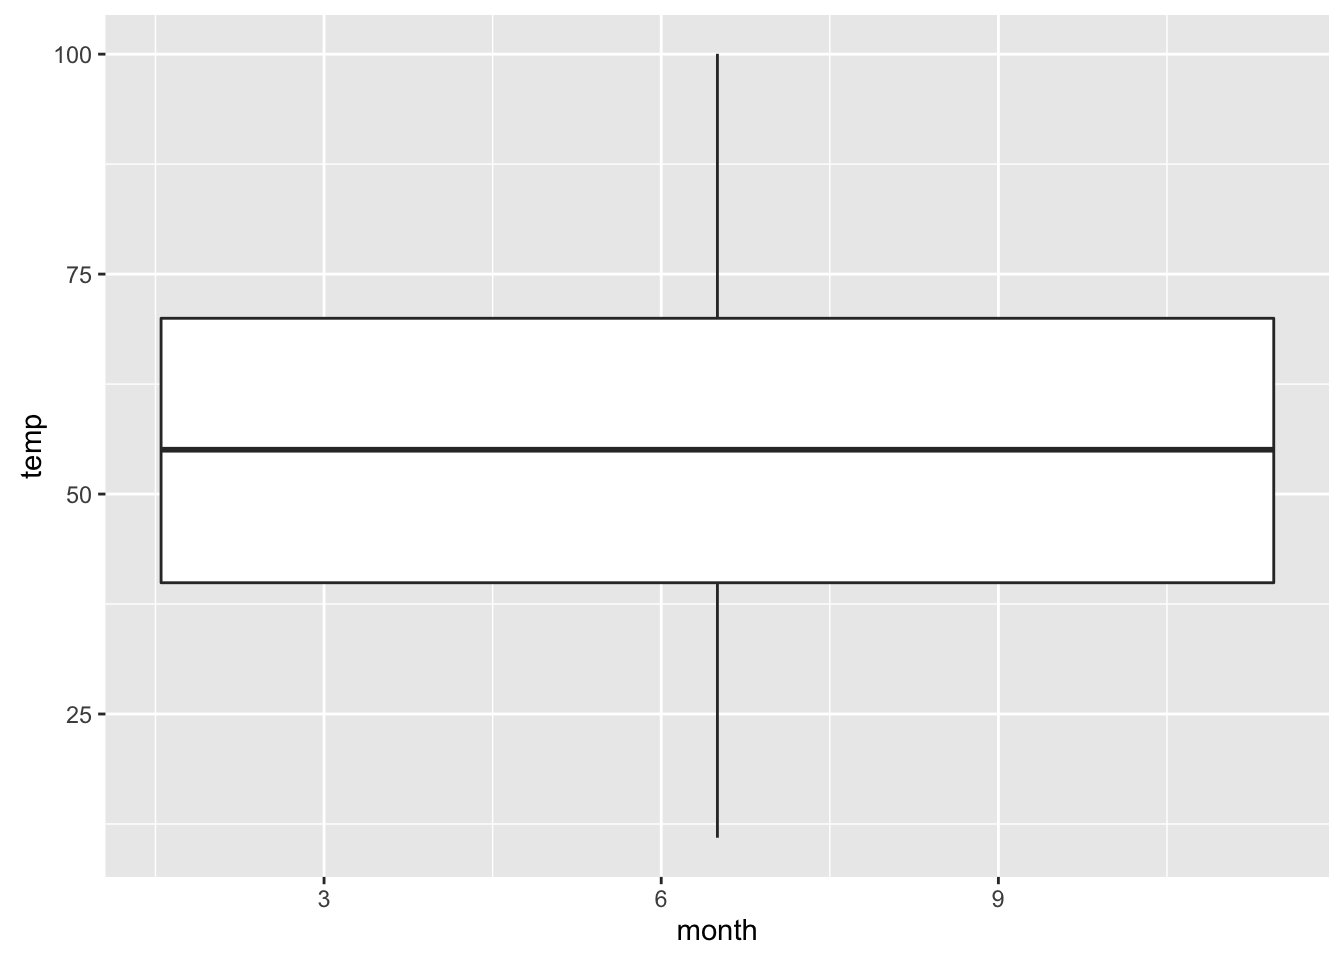
\includegraphics[width=\textwidth]{ismay_files/figure-latex/badbox-1} 

}

\caption[Invalid boxplot specification]{Invalid boxplot specification}\label{fig:badbox}
\end{figure}

Note the first warning that is given here. (The second one corresponds
to missing values in the dataframe and it is turned off on subsequent
plots.) This plot does not look like what we were expecting. We were
expecting to see the distribution of temperatures for each month (so 12
different boxplots). This gives us the overall boxplot without any other
groupings. We can get around this by introducing a new function for our
\texttt{x} variable.

\begin{Shaded}
\begin{Highlighting}[]
\KeywordTok{ggplot}\NormalTok{(}\DataTypeTok{data =} \NormalTok{weather, }\DataTypeTok{mapping =} \KeywordTok{aes}\NormalTok{(}\DataTypeTok{x =} \KeywordTok{factor}\NormalTok{(month), }\DataTypeTok{y =} \NormalTok{temp)) +}
\StringTok{  }\KeywordTok{geom_boxplot}\NormalTok{()}
\end{Highlighting}
\end{Shaded}

\begin{figure}

{\centering 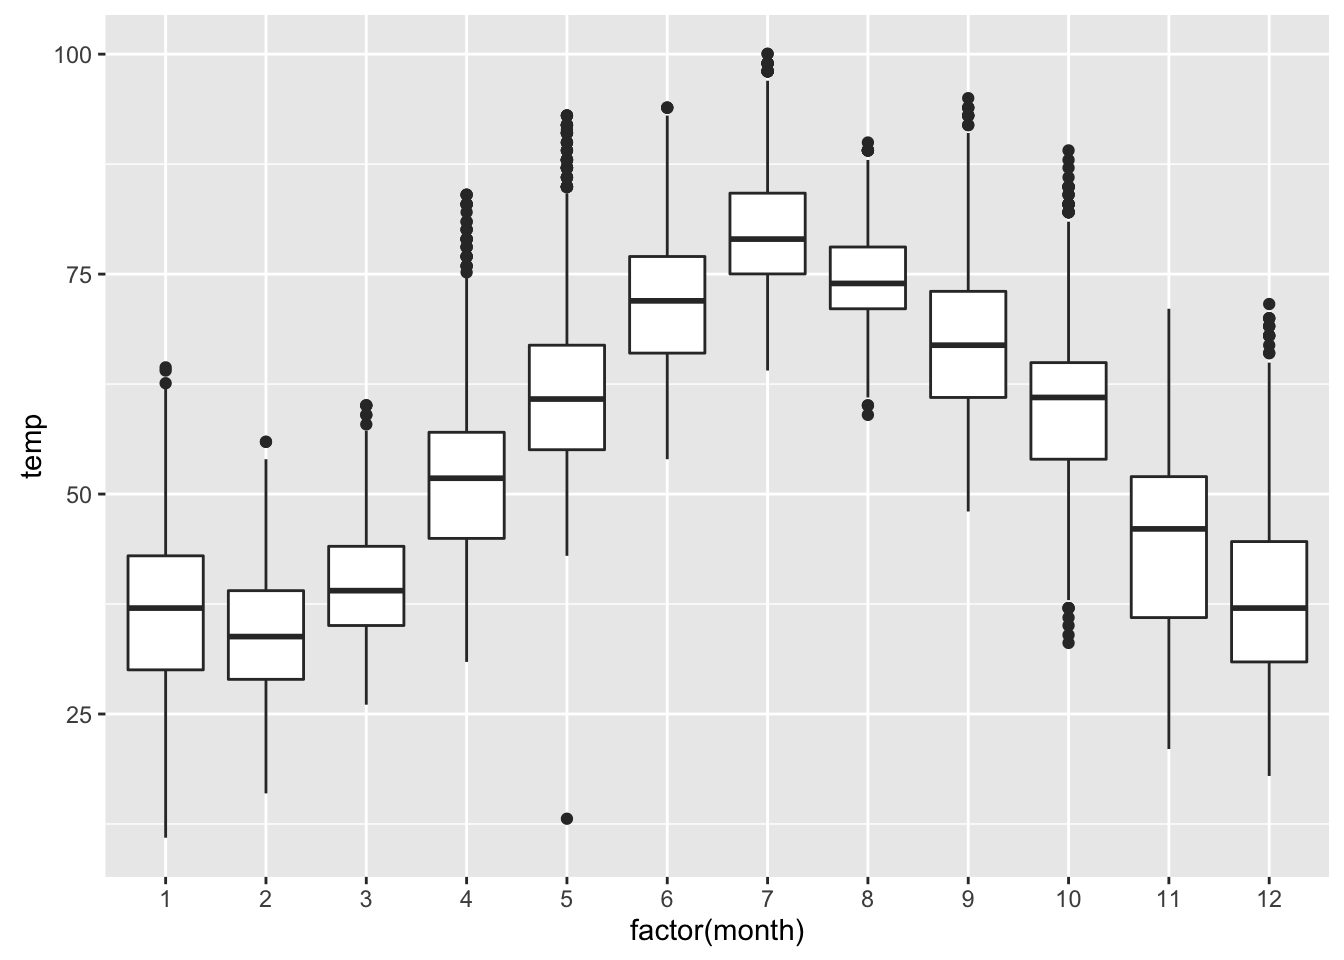
\includegraphics[width=\textwidth]{ismay_files/figure-latex/monthtempbox-1} 

}

\caption[Month by temp boxplot]{Month by temp boxplot}\label{fig:monthtempbox}
\end{figure}

We have introduced a new function called \texttt{factor()} here. One of
the things this function does is to convert a numeric value like
\texttt{month} (1, 2, \ldots{}, 12) into a categorical variable. The
``box'' part of this plot represents the 25\textsuperscript{th}
percentile, the median (50\textsuperscript{th} percentile), and the
75\textsuperscript{th} percentile. The dots correspond to
\textbf{outliers}. (The specific formulation for these outliers is
discussed in Appendix B - Chapter \ref{appendix2}.) The lines show how
the data varies that is not in the center 50\% defined by the first and
third quantiles. Longer lines correspond to more variability and shorter
lines correspond to less variability.

\begin{center}\rule{0.5\linewidth}{\linethickness}\end{center}

\begin{learncheck}
\textbf{\emph{Learning check}}
\end{learncheck}

\textbf{(LC4.10)} What does the dot at the bottom of the plot for May
correspond to? Explain what might have occurred in May to produce this
point.

\textbf{(LC4.11)} Which months have the highest variability in
temperature? What reasons do you think this is?

\textbf{(LC4.12)} We looked at the distribution of a continuous variable
over a categorical variable here with this boxplot. Why can't we look at
the distribution of one continuous variable over the distribution of
another continuous variable? Say temperature across pressure, for
example?

\textbf{(LC4.13)} Boxplots provide a simple way to identify outliers.
Why may outliers be easier to identify when looking at a boxplot instead
of a faceted histogram?

\begin{center}\rule{0.5\linewidth}{\linethickness}\end{center}

\subsection{Summary}\label{summary-1}

Boxplots provide a way to compare and contrast the distribution of ONE
quantitative variable across multiple levels of ONE categorical
variable. One can easily look to see where the median falls across the
different groups by looking at the center line in the box. You can also
see how spread out the variable is across the different groups by
looking at the width of the box and also how far out the lines stretch
from the box. Lastly, outliers are even more easily identified when
looking at a boxplot than when looking at a histogram.

\section{Barplots}\label{barplots}

Both histograms and boxplots represent ways to visualize the variability
of continuous variables. Another common task is to present the
distribution of a categorical variable. This is a simpler task since we
will be interested in how many elements from our data fall into the
different categories of the categorical variable. We need not bin the
data or identify the different quantiles for categorical variables.

Frequently, the best way to visualize these different counts (also known
as \textbf{frequencies}) is via a barplot. Consider the distribution of
airlines that flew out of New York City in 2013. This can be plotted by
invoking the \texttt{geom\_bar} function in \texttt{ggplot2}:

\begin{Shaded}
\begin{Highlighting}[]
\KeywordTok{ggplot}\NormalTok{(}\DataTypeTok{data =} \NormalTok{flights, }\DataTypeTok{mapping =} \KeywordTok{aes}\NormalTok{(}\DataTypeTok{x =} \NormalTok{carrier)) +}
\StringTok{  }\KeywordTok{geom_bar}\NormalTok{()}
\end{Highlighting}
\end{Shaded}

\begin{figure}

{\centering 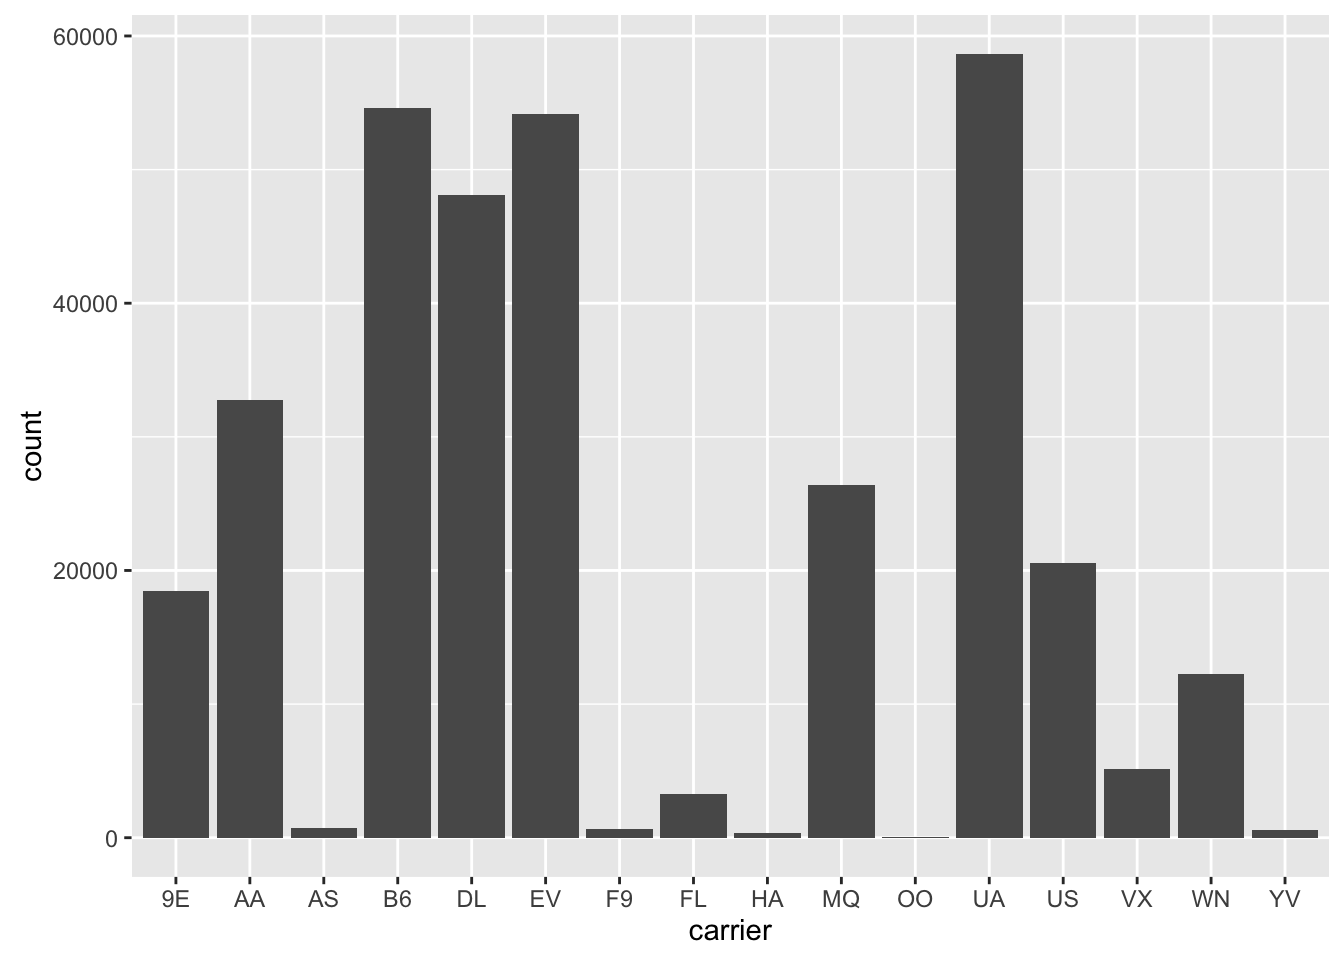
\includegraphics[width=\textwidth]{ismay_files/figure-latex/flightsbar-1} 

}

\caption[Number of flights departing NYC in 2013 by airline]{Number of flights departing NYC in 2013 by airline}\label{fig:flightsbar}
\end{figure}

Recall the \texttt{airlines} dataset discussed in Chapter \ref{tidy}.

\begin{Shaded}
\begin{Highlighting}[]
\KeywordTok{data}\NormalTok{(airlines)}
\NormalTok{airlines}
\end{Highlighting}
\end{Shaded}

\begin{verbatim}
## # A tibble: 16 x 2
##    carrier                        name
##      <chr>                       <chr>
## 1       9E           Endeavor Air Inc.
## 2       AA      American Airlines Inc.
## 3       AS        Alaska Airlines Inc.
## 4       B6             JetBlue Airways
## 5       DL        Delta Air Lines Inc.
## 6       EV    ExpressJet Airlines Inc.
## 7       F9      Frontier Airlines Inc.
## 8       FL AirTran Airways Corporation
## 9       HA      Hawaiian Airlines Inc.
## 10      MQ                   Envoy Air
## 11      OO       SkyWest Airlines Inc.
## 12      UA       United Air Lines Inc.
## 13      US             US Airways Inc.
## 14      VX              Virgin America
## 15      WN      Southwest Airlines Co.
## 16      YV          Mesa Airlines Inc.
\end{verbatim}

We see that United Air Lines, JetBlue Airways, and ExpressJet Airlines
had the most flights depart New York City in 2013. To get the actual
number of flights by each airline we can use the \texttt{count} function
in the \texttt{dplyr} package on the \texttt{carrier} variable in
\texttt{flights}:

\begin{Shaded}
\begin{Highlighting}[]
\KeywordTok{library}\NormalTok{(dplyr)}
\NormalTok{flights_table <-}\StringTok{ }\KeywordTok{count}\NormalTok{(}\DataTypeTok{x =} \NormalTok{flights, }\DataTypeTok{vars =} \NormalTok{carrier)}
\NormalTok{flights_table}
\end{Highlighting}
\end{Shaded}

\begin{verbatim}
## # A tibble: 16 x 2
##     vars     n
##    <chr> <int>
## 1     9E 18460
## 2     AA 32729
## 3     AS   714
## 4     B6 54635
## 5     DL 48110
## 6     EV 54173
## 7     F9   685
## 8     FL  3260
## 9     HA   342
## 10    MQ 26397
## 11    OO    32
## 12    UA 58665
## 13    US 20536
## 14    VX  5162
## 15    WN 12275
## 16    YV   601
\end{verbatim}

\begin{center}\rule{0.5\linewidth}{\linethickness}\end{center}

\begin{learncheck}
\textbf{\emph{Learning check}}
\end{learncheck}

\textbf{(LC4.14)} Why are histograms inappropriate for visualizing
categorical variables?

\textbf{(LC4.15)} What is the difference between histograms and
barplots?

\textbf{(LC4.16)} How many Envoy Air flights departed NYC in 2013?

\textbf{(LC4.17)} What was the seventh highest airline in terms of
departed flights from NYC in 2013?

\begin{center}\rule{0.5\linewidth}{\linethickness}\end{center}

\subsection{Must avoid pie charts!}\label{must-avoid-pie-charts}

Unfortunately, one of the most common plots seen today for categorical
data is the pie chart. While they may see harmless enough, they actually
present a problem in that humans are unable to judge angles well. As
Naomi Robbins describes in her book ``Creating More Effective Graphs'',
we overestimate angles greater than 90 degrees and we underestimate
angles less than 90 degrees. In other words, it is difficult for us to
determine relative size of one piece of the pie compared to another.

Let's examine our previous barplot example on the number of flights
departing NYC by airline. This time we will use a pie chart. As you
review this chart, try to identify

\begin{itemize}
\tightlist
\item
  how much larger the portion of the pie is for ExpressJet Airlines
  (\texttt{EV}) compared to US Airways (\texttt{US}),
\item
  what the third largest carrier is in terms of departing flights, and
\item
  how many carriers have fewer flights than United Airlines
  (\texttt{UA})?
\end{itemize}

\begin{figure}

{\centering 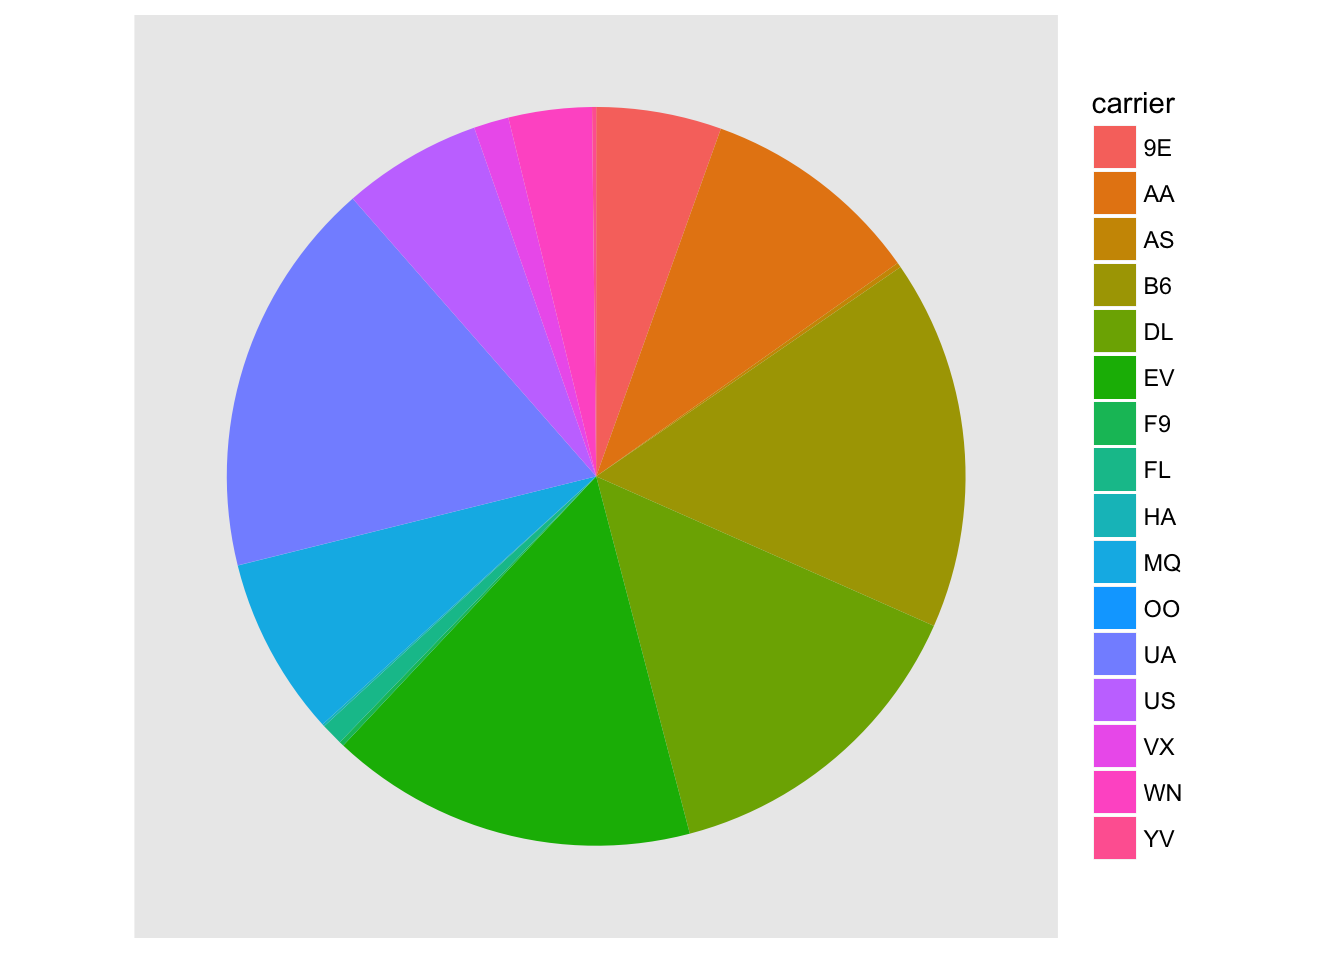
\includegraphics[width=\textwidth]{ismay_files/figure-latex/carrierpie-1} 

}

\caption[The dreaded pie chart]{The dreaded pie chart}\label{fig:carrierpie}
\end{figure}

While it is quite easy to look back at the barplot to get the answer to
these questions, it's quite difficult to get the answers correct when
looking at the pie graph. Barplots can always present the information in
a way that is easier for the eye to determine relative position. There
may be one exception from Nathan Yau at
\href{https://flowingdata.com/2008/09/19/pie-i-have-eaten-and-pie-i-have-not-eaten/}{FlowingData.com}
but we will leave this for the reader to decide:

\begin{figure}

{\centering 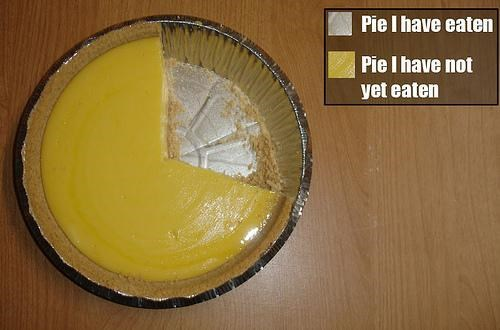
\includegraphics[width=\textwidth]{images/Pie-I-have-Eaten} 

}

\caption[The only good pie chart]{The only good pie chart}\label{fig:unnamed-chunk-25}
\end{figure}

\begin{center}\rule{0.5\linewidth}{\linethickness}\end{center}

\begin{learncheck}
\textbf{\emph{Learning check}}
\end{learncheck}

\textbf{(LC4.18)} Why should pie charts be avoided and replaced by
barplots?

\textbf{(LC4.19)} What is your opinion as to why pie charts continue to
be used?

\begin{center}\rule{0.5\linewidth}{\linethickness}\end{center}

\subsection{Using barplots to compare two
variables}\label{using-barplots-to-compare-two-variables}

Barplots are the go-to way to visualize the frequency of different
categories of a categorical variable. They make it easy to order the
counts and to compare one group's frequency to another. Another use of
barplots (unfortunately, sometimes inappropriately and confusingly) is
to compare two categorical variables together. Let's examine the
distribution of outgoing flights from NYC by \texttt{carrier} and
\texttt{airport}.

We begin by getting the names of the airports in NYC that were included
in the \texttt{flights} dataset. Remember from Chapter \ref{tidy} that
this can be done by using the \texttt{inner\_join} function in the
\texttt{dplyr} package.

\begin{Shaded}
\begin{Highlighting}[]
\KeywordTok{library}\NormalTok{(dplyr)}
\NormalTok{flights_namedports <-}\StringTok{ }\KeywordTok{inner_join}\NormalTok{(flights, airports, }\DataTypeTok{by =} \KeywordTok{c}\NormalTok{(}\StringTok{"origin"} \NormalTok{=}\StringTok{ "faa"}\NormalTok{))}
\end{Highlighting}
\end{Shaded}

After running \texttt{View(flights\_namedports)}, we see that
\texttt{name} now corresponds to the name of the airport as referenced
by the \texttt{origin} variable. We will now plot \texttt{carrier} as
the horizontal variable. When we specify \texttt{geom\_bar}, it will
specify \texttt{count} as being the vertical variable. A new addition
here is \texttt{fill\ =\ name}. Look over what was produced from the
plot to get an idea of what this argument gives.

\begin{Shaded}
\begin{Highlighting}[]
\KeywordTok{ggplot}\NormalTok{(}\DataTypeTok{data =} \NormalTok{flights_namedports, }\DataTypeTok{mapping =} \KeywordTok{aes}\NormalTok{(}\DataTypeTok{x =} \NormalTok{carrier, }\DataTypeTok{fill =} \NormalTok{name)) +}
\StringTok{  }\KeywordTok{geom_bar}\NormalTok{()}
\end{Highlighting}
\end{Shaded}

\begin{figure}

{\centering 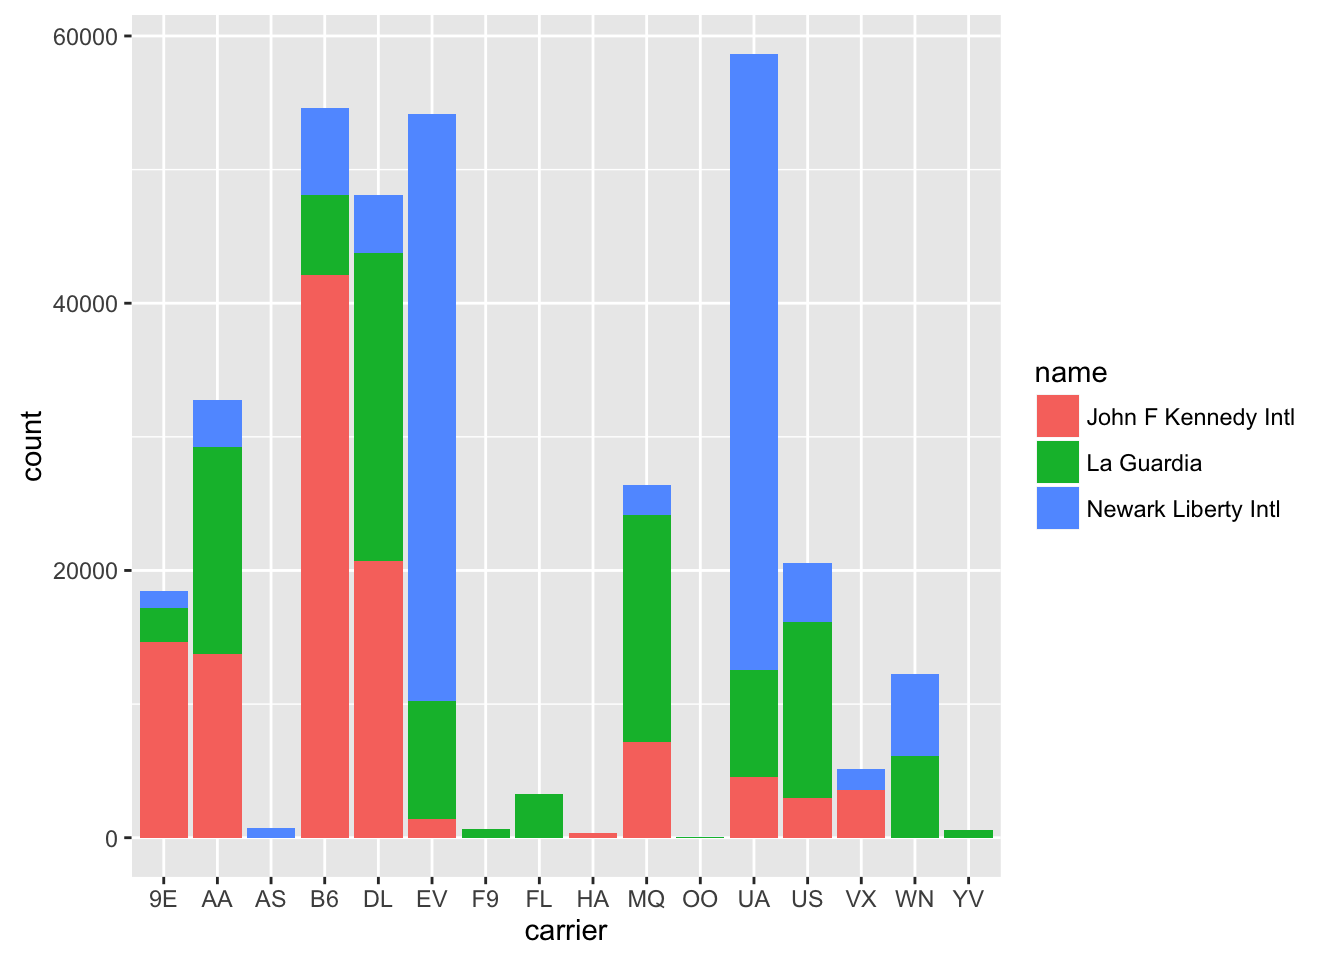
\includegraphics[width=\textwidth]{ismay_files/figure-latex/unnamed-chunk-27-1} 

}

\caption[Stacked barplot comparing the number of flights by carrier and airport]{Stacked barplot comparing the number of flights by carrier and airport}\label{fig:unnamed-chunk-27}
\end{figure}

This plot is what is known as a \textbf{stacked barplot}. While simple
to make, it often leads to many problems.

\begin{learncheck}
\textbf{\emph{Learning check}}
\end{learncheck}

\textbf{(LC4.20)} What kinds of questions are not easily answered by
looking at the above figure?

\textbf{(LC4.21)} What can you say, if anything, about the relationship
between airline and airport in NYC in 2013 in regards to the number of
departing flights?

\begin{center}\rule{0.5\linewidth}{\linethickness}\end{center}

Another variation on the \textbf{stacked barplot} is the
\textbf{side-by-side barplot}.

\begin{Shaded}
\begin{Highlighting}[]
\KeywordTok{ggplot}\NormalTok{(}\DataTypeTok{data =} \NormalTok{flights_namedports, }\DataTypeTok{mapping =} \KeywordTok{aes}\NormalTok{(}\DataTypeTok{x =} \NormalTok{carrier, }\DataTypeTok{fill =} \NormalTok{name)) +}
\StringTok{  }\KeywordTok{geom_bar}\NormalTok{(}\DataTypeTok{position =} \StringTok{"dodge"}\NormalTok{)}
\end{Highlighting}
\end{Shaded}

\begin{figure}

{\centering 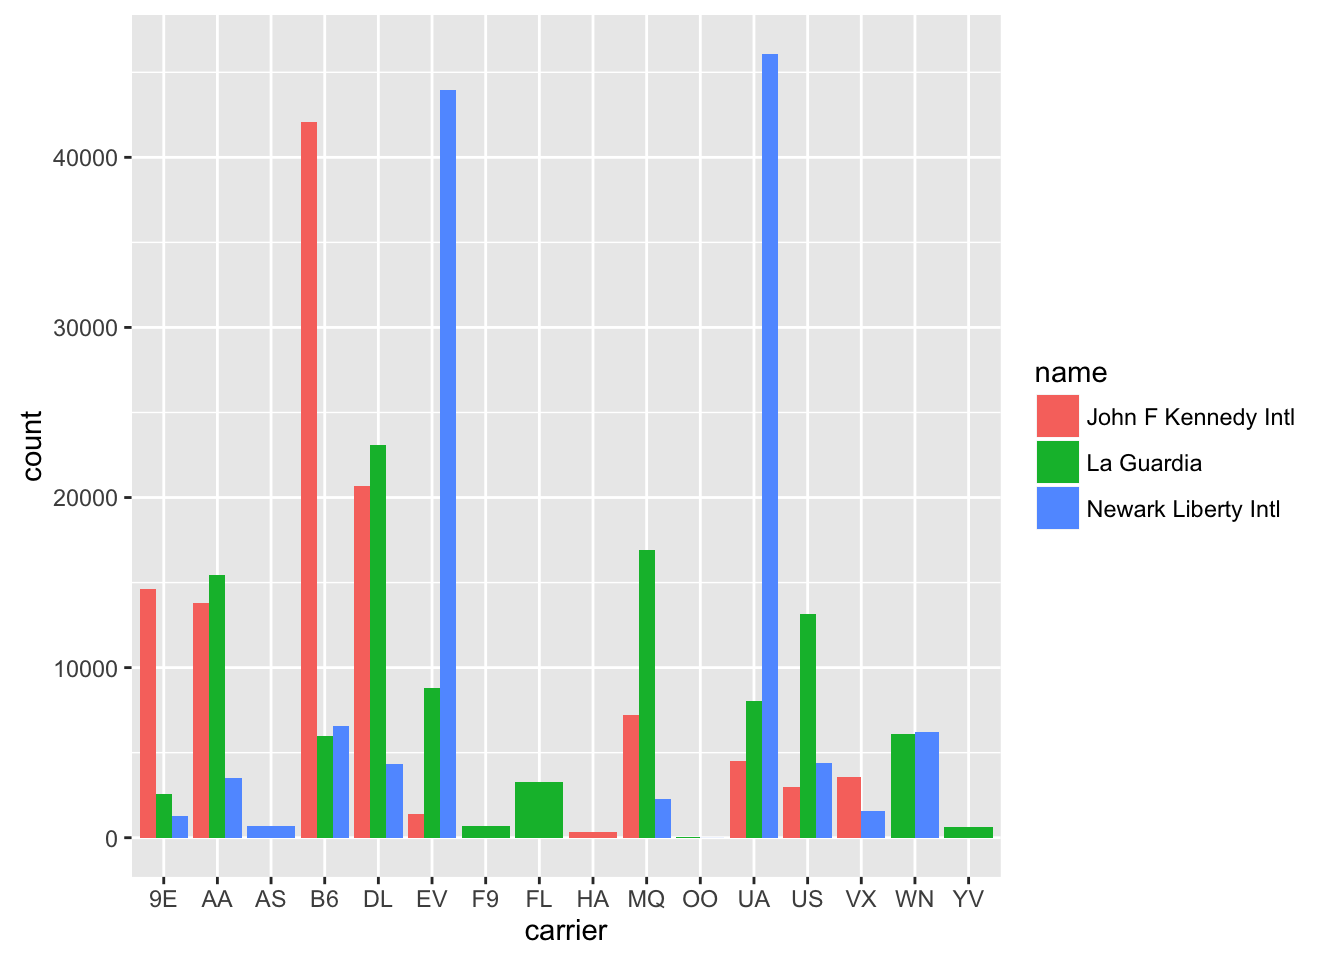
\includegraphics[width=\textwidth]{ismay_files/figure-latex/unnamed-chunk-28-1} 

}

\caption[Side-by-side barplot comparing the number of flights by carrier and airport]{Side-by-side barplot comparing the number of flights by carrier and airport}\label{fig:unnamed-chunk-28}
\end{figure}

\begin{center}\rule{0.5\linewidth}{\linethickness}\end{center}

\begin{learncheck}
\textbf{\emph{Learning check}}
\end{learncheck}

\textbf{(LC4.22)} Why might the side-by-side barplot be preferable to a
stacked barplot in this case?

\textbf{(LC4.23)} What are the disadvantages of using a side-by-side
barplot, in general?

\begin{center}\rule{0.5\linewidth}{\linethickness}\end{center}

Lastly, an often preferred type of barplot is the \textbf{faceted
barplot}. We already saw this concept of faceting and small multiples in
Subsection \ref{faceting}. This gives us a nicer way to compare the
distributions across both \texttt{carrier} and airport/\texttt{name}.

\begin{Shaded}
\begin{Highlighting}[]
\KeywordTok{ggplot}\NormalTok{(}\DataTypeTok{data =} \NormalTok{flights_namedports, }\DataTypeTok{mapping =} \KeywordTok{aes}\NormalTok{(}\DataTypeTok{x =} \NormalTok{carrier, }\DataTypeTok{fill =} \NormalTok{name)) +}
\StringTok{  }\KeywordTok{geom_bar}\NormalTok{() +}
\StringTok{  }\KeywordTok{facet_grid}\NormalTok{(name ~}\StringTok{ }\NormalTok{.)}
\end{Highlighting}
\end{Shaded}

\begin{figure}

{\centering 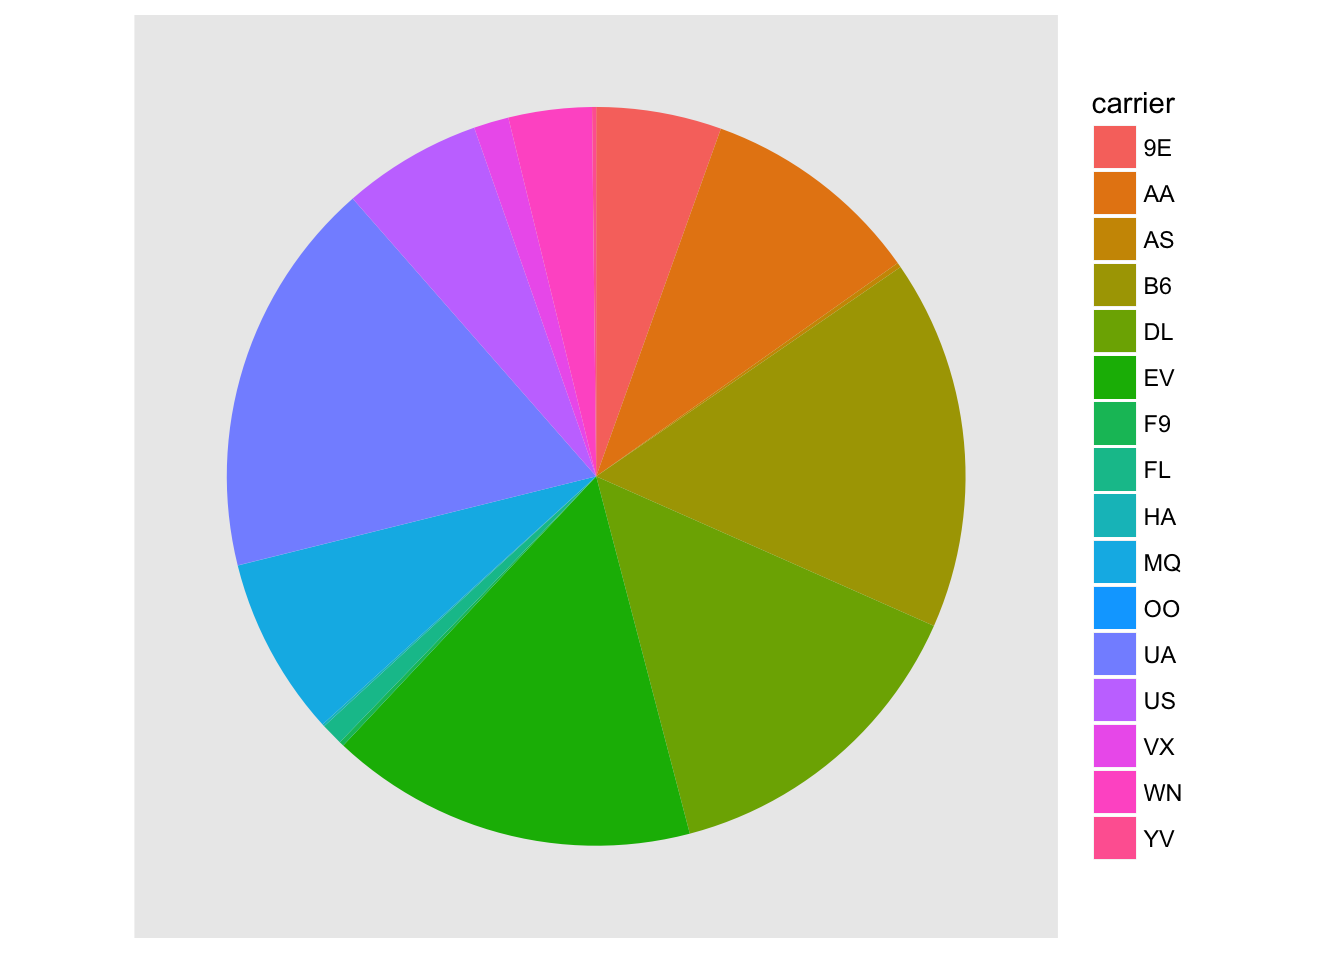
\includegraphics[width=\textwidth]{ismay_files/figure-latex/unnamed-chunk-29-1} 

}

\caption[Faceted barplot comparing the number of flights by carrier and airport]{Faceted barplot comparing the number of flights by carrier and airport}\label{fig:unnamed-chunk-29}
\end{figure}

Note how the \texttt{facet\_grid} function arguments are written here.
We are wanting the names of the airports vertically and the
\texttt{carrier} listed horizontally. As you may have guessed, this
argument and other \emph{formulas} of this sort in R are in
\texttt{y\ \textasciitilde{}\ x} order. We will see more examples of
this in Chapter \ref{regress}.

\begin{center}\rule{0.5\linewidth}{\linethickness}\end{center}

\begin{learncheck}
\textbf{\emph{Learning check}}
\end{learncheck}

\textbf{(LC4.24)} Why is the faceted barplot preferred to the
side-by-side and stacked barplots in this case?

\textbf{(LC4.25)} What information about the different carriers at
different airports is more easily seen in the faceted barplot?

\begin{center}\rule{0.5\linewidth}{\linethickness}\end{center}

\subsection{Summary}\label{summary-2}

Barplots are the preferred way of displaying categorical variables. They
are easy-to-understand and to make comparisons across groups of a
categorical variable. When dealing with more than one categorical
variable, faceted barplots are frequently preferred over side-by-side or
stacked barplots. Stacked barplots are sometimes nice to look at, but it
is quite difficult to compare across the levels since the sizes of the
bars are all of different sizes. Side-by-side barplots can provide an
improvement on this, but the issue about comparing across groups still
must be dealt with.

\section{Scatter-plots}\label{scatter-plots}

We have seen that boxplots are most appropriate when plotting the
distribution of ONE continuous variable across different levels/groups
of ONE categorical variable. Barplots (preferably the faceted type) are
best when looking at the distribution of ONE categorical variable across
different levels of another categorical variable. But what if we are
looking to investigate the relationship between TWO continuous
variables? What is commonly produced is the well-known
\textbf{scatter-plot}, which shows the points corresponding to the
values of each of the variables scattered around.

We will now investigate arrival delays (the vertical ``y'' axis
variable) versus departure delays (the horizontal ``x'' axis variable)
for Alaska Airlines flights leaving NYC in 2013. Notice the new function
that is invoked here: \texttt{filter}, which resides in the
\texttt{dplyr} package. You will see many more examples using this
function in Chapter \ref{manip}. The \texttt{filter} function goes
through the dataframe specified (\texttt{flights} here) and selects only
those rows which meet the condition given (\texttt{carrier\ ==\ "AS"}
here).

\begin{Shaded}
\begin{Highlighting}[]
\NormalTok{alaska_flights <-}\StringTok{ }\KeywordTok{filter}\NormalTok{(flights, carrier ==}\StringTok{ "AS"}\NormalTok{)}
\KeywordTok{ggplot}\NormalTok{(alaska_flights, }\KeywordTok{aes}\NormalTok{(}\DataTypeTok{x =} \NormalTok{dep_delay, }\DataTypeTok{y =} \NormalTok{arr_delay)) +}\StringTok{ }
\StringTok{  }\KeywordTok{geom_point}\NormalTok{()}
\end{Highlighting}
\end{Shaded}

\begin{figure}

{\centering 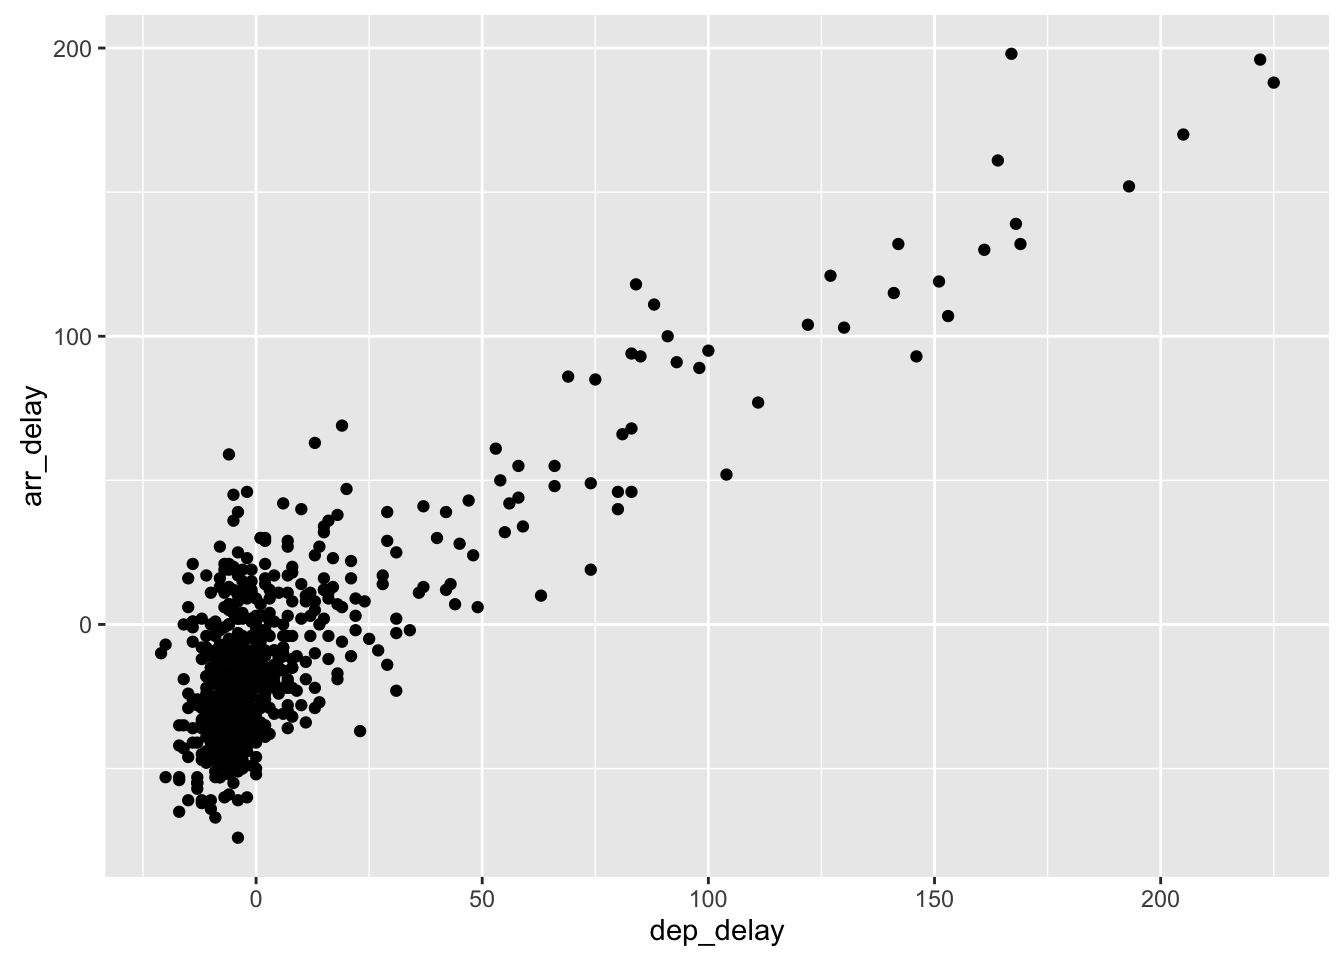
\includegraphics[width=\textwidth]{ismay_files/figure-latex/noalpha-1} 

}

\caption[Arrival Delays vs Departure Delays for Alaska Airlines flights from NYC in 2013]{Arrival Delays vs Departure Delays for Alaska Airlines flights from NYC in 2013}\label{fig:noalpha}
\end{figure}

We see that a positive relationship exists between \texttt{dep\_delay}
and \texttt{arr\_delay}: as departure delays increase, arrival delays
tend to also increase. We also note that the majority of points fall
near the point (0, 0) here. There is a large mass of points clustered
there.

\begin{center}\rule{0.5\linewidth}{\linethickness}\end{center}

\begin{learncheck}
\textbf{\emph{Learning check}}
\end{learncheck}

\textbf{(LC4.26)} What are some practical reasons why
\texttt{dep\_delay} and \texttt{arr\_delay} have a positive
relationship?

\textbf{(LC4.27)} What variables (not necessarily in the
\texttt{flights} dataframe) would you expect to have a negative
correlation (i.e.~a negative relationship) with \texttt{dep\_delay}?
Why? Remember that we are focusing on continuous variables here.

\textbf{(LC4.28)} Why do you believe there is a cluster of points near
(0, 0)?

\begin{itemize}
\tightlist
\item
  What does (0, 0) correspond to in terms of the Alaskan flights?
\end{itemize}

\textbf{(LC4.29)} What are some other features of the plot that stand
out to you?

\begin{center}\rule{0.5\linewidth}{\linethickness}\end{center}

\subsection{Jittering}\label{jittering}

The large mass of points near (0, 0) can cause some confusion. This is
the result of a phenomenon called \textbf{over-plotting}. As one may
guess, this corresponds to values being plotted on top of each other
\emph{over} and \emph{over} again. It is often difficult to know just
how many values are plotted in this way when looking at a basic
scatter-plot as we have here.

One way of relieving this issue of \textbf{over-plotting} is to
\textbf{jitter} the points a bit. In other words, we are going to add
just a bit of random noise to the points to better see them and remove
some of the over-plotting. You can think of ``jittering'' as shaking the
points a bit on the plot. Instead of using \texttt{geom\_point}, we use
\texttt{geom\_jitter} to perform this shaking and specify around how
much jitter to add with the \texttt{width} and \texttt{height}
arguments. This corresponds to how hard you'd like to shake the plot in
units corresponding to those for both the horizontal and vertical
variables (minutes here).

\begin{Shaded}
\begin{Highlighting}[]
\KeywordTok{ggplot}\NormalTok{(alaska_flights, }\KeywordTok{aes}\NormalTok{(}\DataTypeTok{x =} \NormalTok{dep_delay, }\DataTypeTok{y =} \NormalTok{arr_delay)) +}\StringTok{ }
\StringTok{  }\KeywordTok{geom_jitter}\NormalTok{(}\DataTypeTok{width =} \DecValTok{30}\NormalTok{, }\DataTypeTok{height =} \DecValTok{30}\NormalTok{)}
\end{Highlighting}
\end{Shaded}

\begin{figure}

{\centering 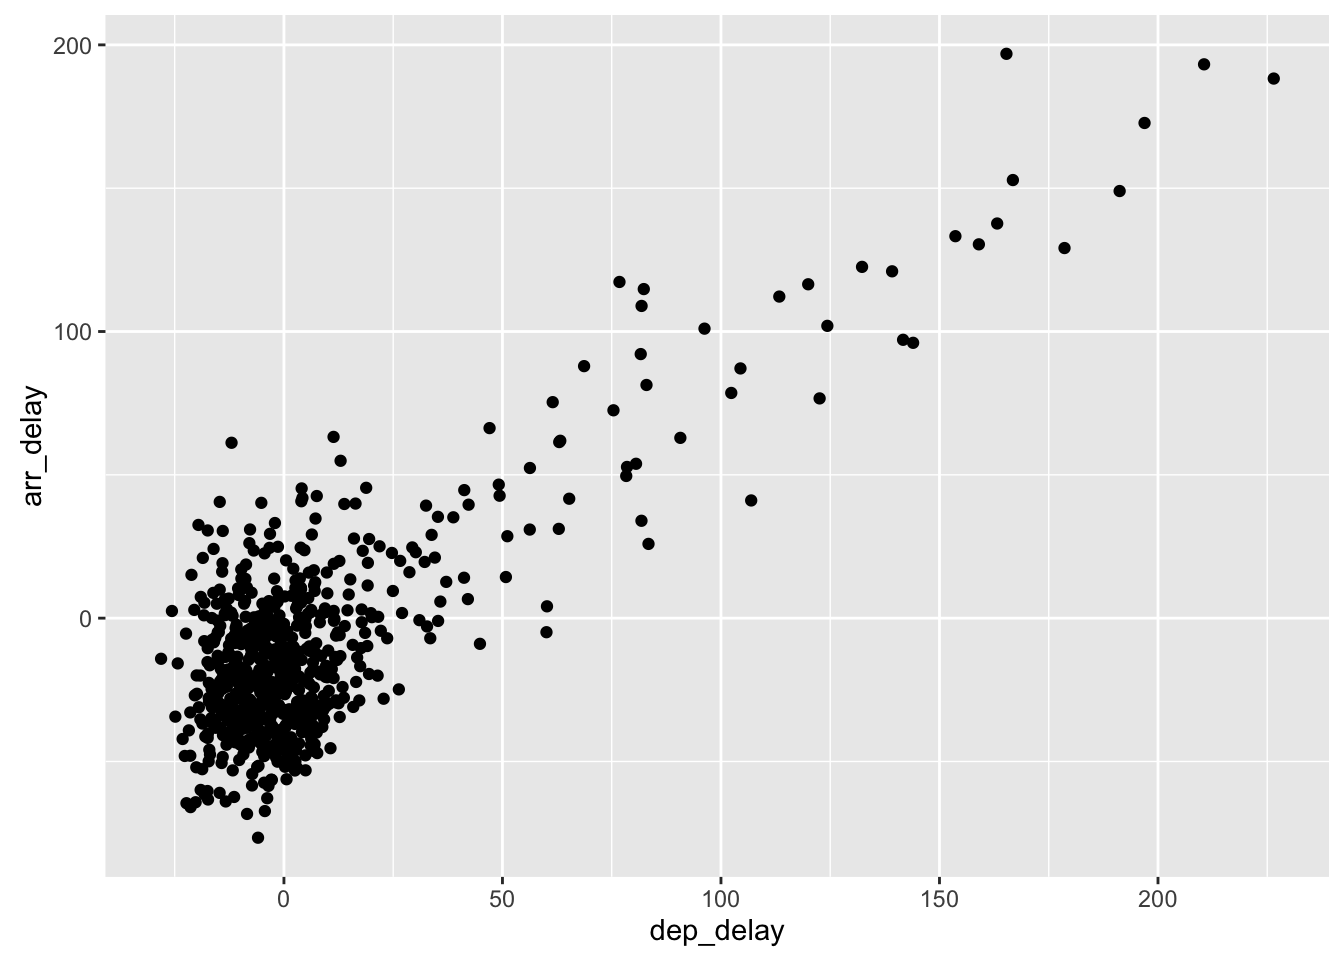
\includegraphics[width=\textwidth]{ismay_files/figure-latex/unnamed-chunk-31-1} 

}

\caption[Jittered delay scatterplot]{Jittered delay scatterplot}\label{fig:unnamed-chunk-31}
\end{figure}

This has helps us a little bit in getting a sense for the over-plotting,
but with a relatively large dataset like this one (714 flights), it is
often useful to change the transparency of the points as seen in the
next section.

\subsection{Setting transparency}\label{setting-transparency}

One of the arguments that can be changed with \texttt{geom\_point} is
\texttt{alpha}. By default, this value is set to \texttt{1}. We can
change this value to a smaller fraction to change the transparency of
the points in the plot:

\begin{Shaded}
\begin{Highlighting}[]
\KeywordTok{ggplot}\NormalTok{(alaska_flights, }\KeywordTok{aes}\NormalTok{(}\DataTypeTok{x =} \NormalTok{dep_delay, }\DataTypeTok{y =} \NormalTok{arr_delay)) +}\StringTok{ }
\StringTok{  }\KeywordTok{geom_point}\NormalTok{(}\DataTypeTok{alpha =} \FloatTok{0.2}\NormalTok{)}
\end{Highlighting}
\end{Shaded}

\begin{figure}

{\centering 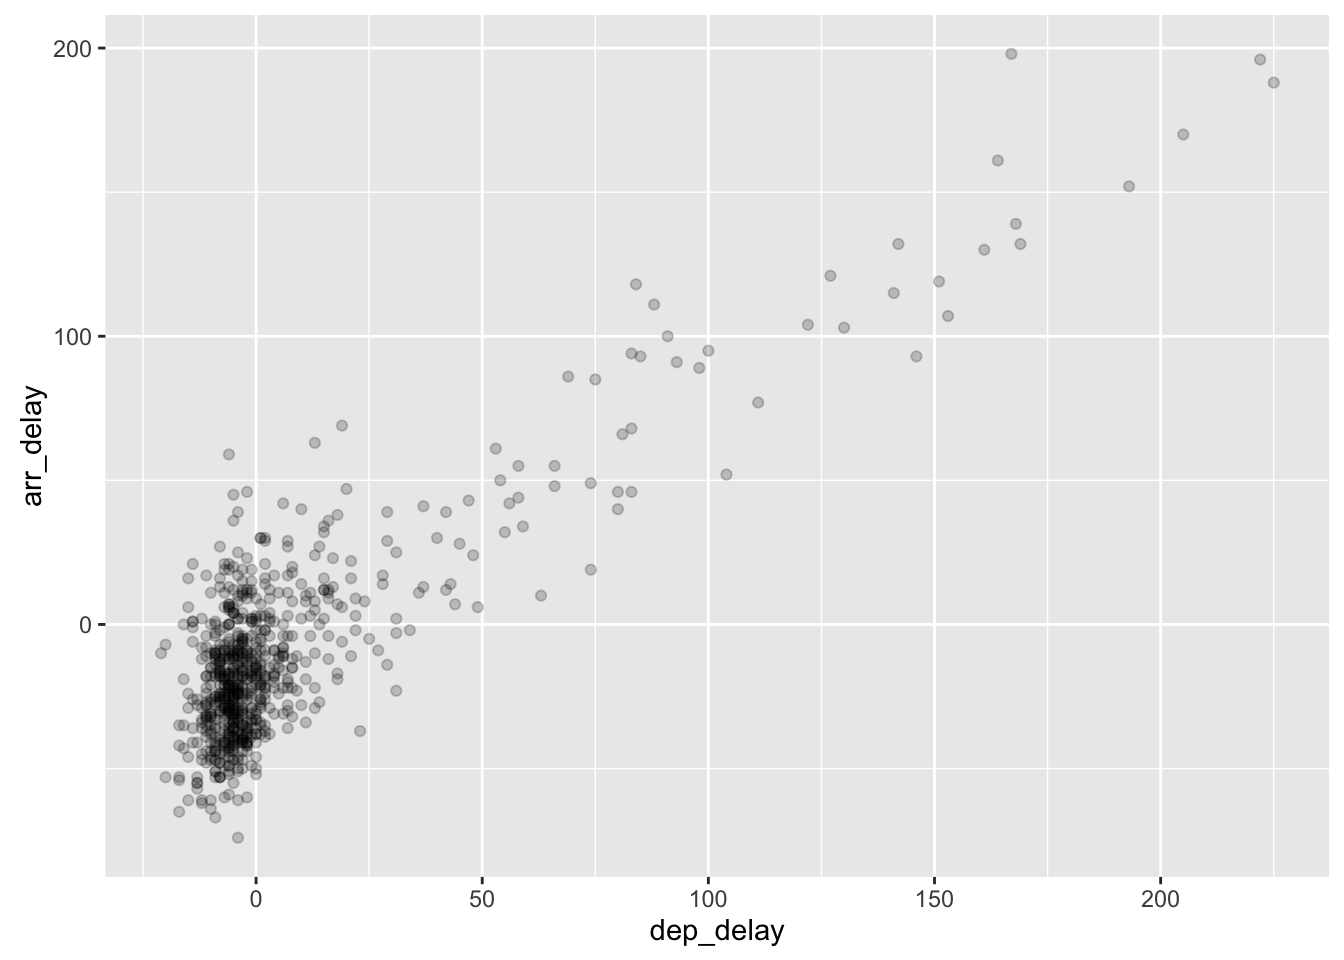
\includegraphics[width=\textwidth]{ismay_files/figure-latex/alpha-1} 

}

\caption[Arrival Delays vs Departure Delays for Alaska Airlines flights from NYC in 2013 - alpha=0.2]{Arrival Delays vs Departure Delays for Alaska Airlines flights from NYC in 2013 - alpha=0.2}\label{fig:alpha}
\end{figure}

We can also specify the \texttt{alpha} argument in
\texttt{geom\_jitter}:

\begin{Shaded}
\begin{Highlighting}[]
\KeywordTok{ggplot}\NormalTok{(alaska_flights, }\KeywordTok{aes}\NormalTok{(}\DataTypeTok{x =} \NormalTok{dep_delay, }\DataTypeTok{y =} \NormalTok{arr_delay)) +}\StringTok{ }
\StringTok{  }\KeywordTok{geom_jitter}\NormalTok{(}\DataTypeTok{width =} \DecValTok{30}\NormalTok{, }\DataTypeTok{height =} \DecValTok{30}\NormalTok{, }\DataTypeTok{alpha =} \FloatTok{0.3}\NormalTok{)}
\end{Highlighting}
\end{Shaded}

\begin{figure}

{\centering 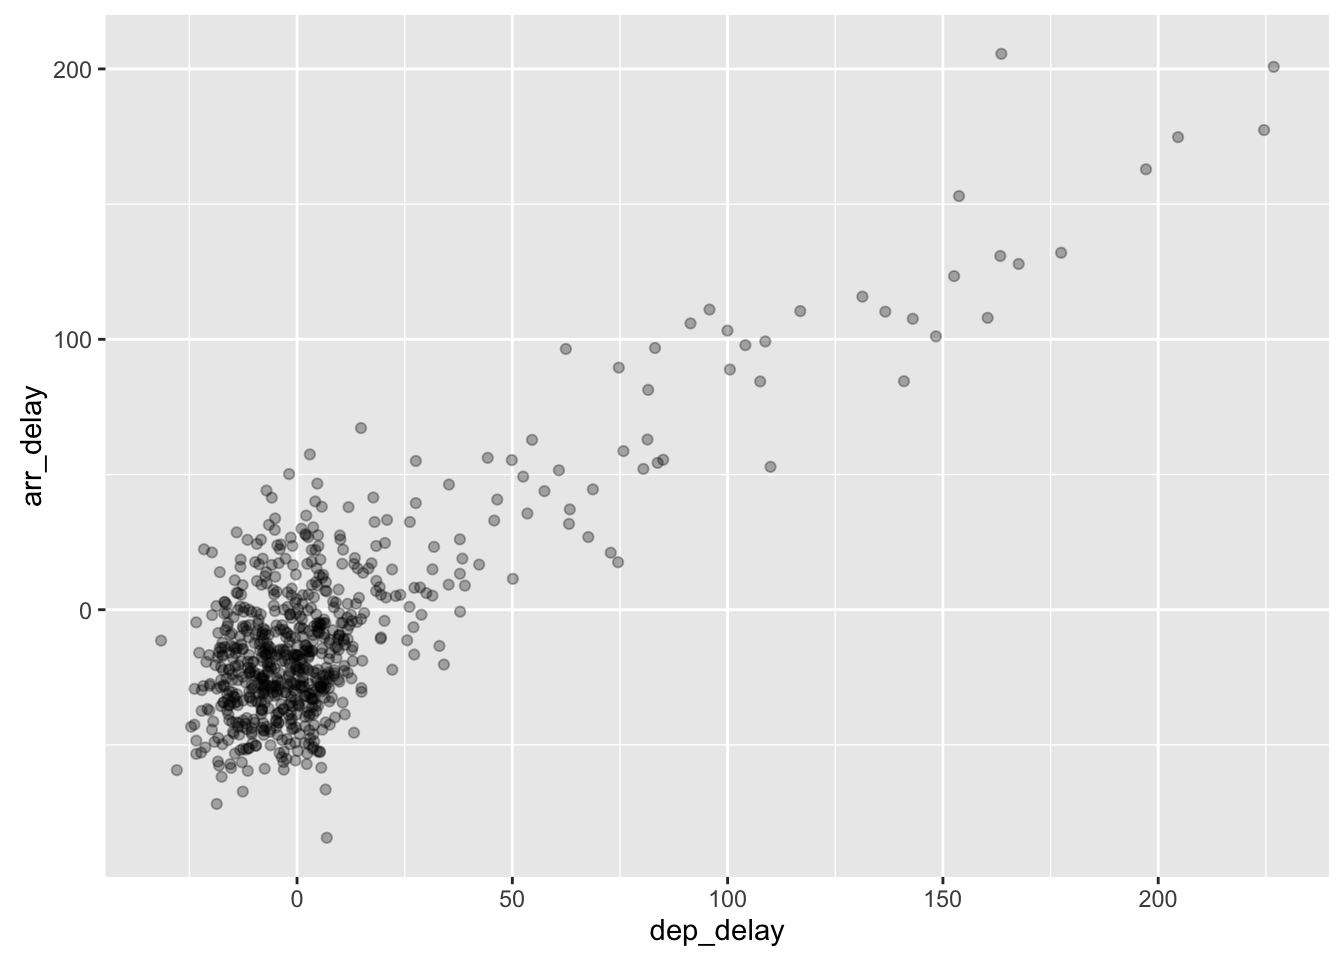
\includegraphics[width=\textwidth]{ismay_files/figure-latex/jitteralpha-1} 

}

\caption[Arrival Delays vs Departure Delays for Alaska Airlines flights from NYC in 2013 - jitter and alpha added]{Arrival Delays vs Departure Delays for Alaska Airlines flights from NYC in 2013 - jitter and alpha added}\label{fig:jitteralpha}
\end{figure}

\begin{center}\rule{0.5\linewidth}{\linethickness}\end{center}

\begin{learncheck}
\textbf{\emph{Learning check}}
\end{learncheck}

\textbf{(LC4.30)} Why is setting the \texttt{alpha} argument value
useful with scatter-plots?

\begin{itemize}
\tightlist
\item
  What further information does it give you that a regular scatter-plot
  cannot?
\end{itemize}

\textbf{(LC4.31)} After viewing the \ref{fig:alpha} above, give a range
of arrival times and departure times that occur most frequently?

\begin{itemize}
\tightlist
\item
  How has that region changed compared to when you observed the same
  plot without the \texttt{alpha\ =\ 0.2} set in \ref{fig:noalpha}?
\end{itemize}

\begin{center}\rule{0.5\linewidth}{\linethickness}\end{center}

\subsection{Summary}\label{summary-3}

Scatter-plots may be the most used plot today and they can provide an
immediate way to see the trend in one variable versus another. Remember
that they only make sense when plotting a continuous variable versus a
continuous variable though. If you try to create a scatter-plot where
either one of the two variables is not quantitative, you will get
strange results. Be careful!

With medium to large datasets, you may need to tweak arguments in both
\texttt{geom\_jitter} and the \texttt{alpha} parameter in order to get a
good feel for relationships in your data. This tweaking is often a fun
part of data visualization since you'll have the chance to see different
relationships come about as you make subtle changes to your plots.

\section{Line-graphs}\label{line-graphs}

The last of the FNG is a line-graph. They are most frequently used when
the horizontal axis is time. Time represents a variable that is
connected together by each day following the previous day. In other
words, time has a natural ordering. Line-graphs should be avoided when
there is not a clear ordering to the explanatory (``x'' variable).

We are interested in exploring the arrival delays by day throughout the
year of 2013 from outgoing flights from New York City. If we plotted all
of these values, we obtain the following scatter-plot:

\begin{Shaded}
\begin{Highlighting}[]
\KeywordTok{ggplot}\NormalTok{(flights, }\KeywordTok{aes}\NormalTok{(}\DataTypeTok{x =} \NormalTok{time_hour, }\DataTypeTok{y =} \NormalTok{arr_delay)) +}\StringTok{ }
\StringTok{  }\KeywordTok{geom_point}\NormalTok{()}
\end{Highlighting}
\end{Shaded}

\begin{figure}

{\centering 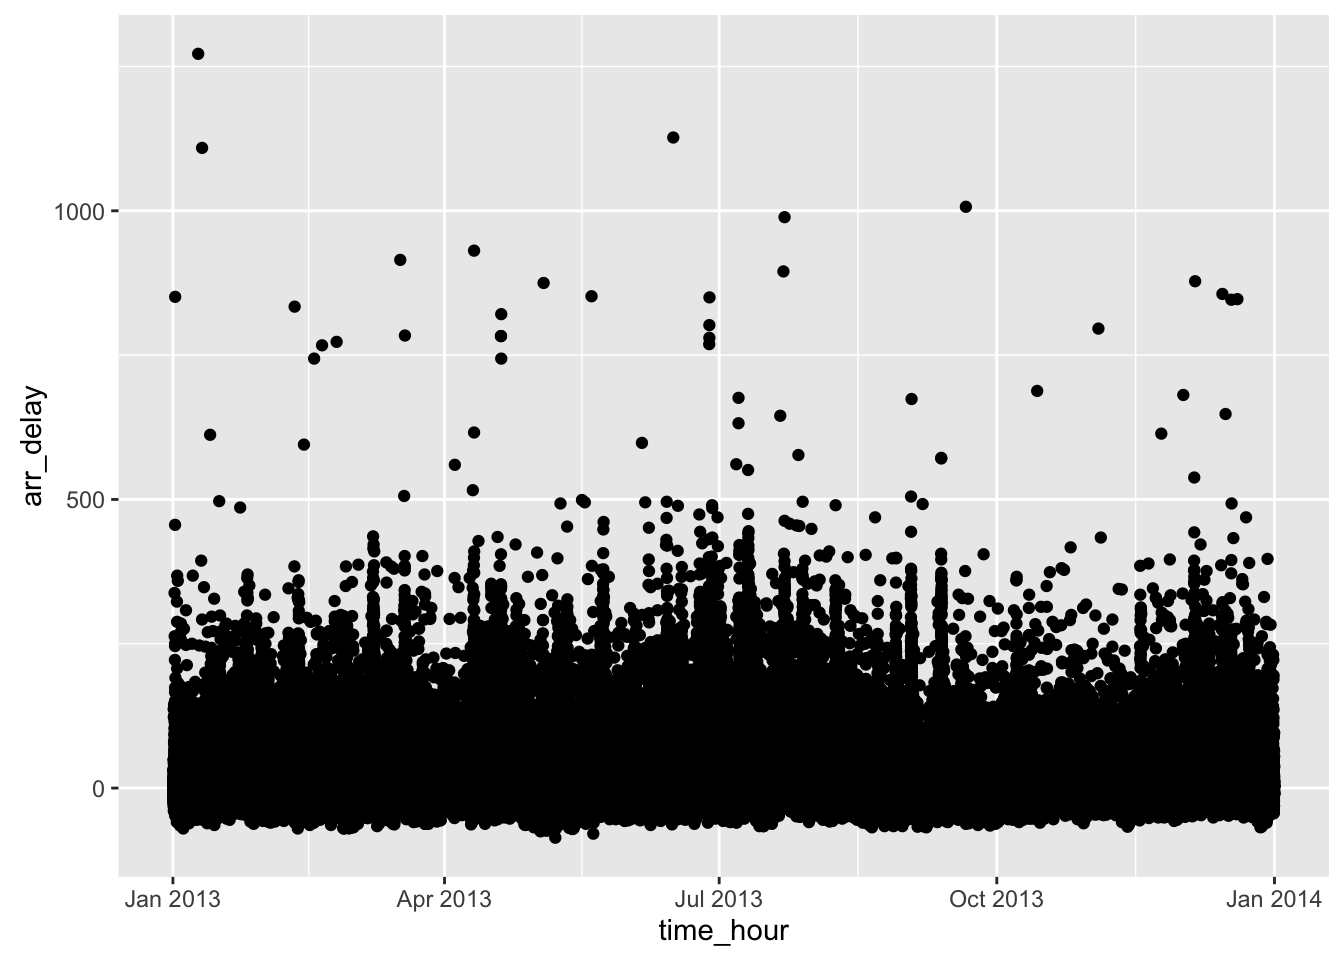
\includegraphics[width=\textwidth]{ismay_files/figure-latex/unnamed-chunk-32-1} 

}

\caption[Hard to read scatterplot]{Hard to read scatterplot}\label{fig:unnamed-chunk-32}
\end{figure}

We see that this plot is difficult to understand based on the sheer
number of points plotted. We see some outlier points with more than 500
minutes of arrival delay, but even some jittering and transparency is
not going to help us here.

Instead of plotting all of the values for each hour for all flights, it
might make sense to plot the average value for each day in terms of
arrival delays. Of course, we also need to address which average we
should use: mean or median. With there being some outliers here, we have
chosen to use the median arrival delay (since the mean is heavily
influence by outliers).

You may think that this is a difficult task but the \texttt{group\_by}
and \texttt{summarize} functions make this a breeze. You'll see more
examples using these two functions in Chapter \ref{manip}. Here we will
create a new variable, which corresponds to the month and day combined,
from the \texttt{time\_hour} column using the \texttt{mutate} function
and create a new dataframe called \texttt{flights\_day}. Notice from
running \texttt{View(flights\_day)} that the new variable added called
\texttt{date} appears on the far right of the dataset.

\begin{Shaded}
\begin{Highlighting}[]
\NormalTok{flights_day <-}\StringTok{ }\KeywordTok{mutate}\NormalTok{(flights, }\DataTypeTok{date =} \KeywordTok{as.Date}\NormalTok{(time_hour))}
\end{Highlighting}
\end{Shaded}

\begin{Shaded}
\begin{Highlighting}[]
\NormalTok{flights_summarized <-}\StringTok{ }\NormalTok{flights_day %>%}\StringTok{ }\KeywordTok{group_by}\NormalTok{(date) %>%}
\StringTok{  }\KeywordTok{summarize}\NormalTok{(}\DataTypeTok{median_arr_delay =} \KeywordTok{median}\NormalTok{(arr_delay, }\DataTypeTok{na.rm =} \OtherTok{TRUE}\NormalTok{))}
\NormalTok{flights_summarized}
\end{Highlighting}
\end{Shaded}

\begin{verbatim}
## # A tibble: 365 x 2
##          date median_arr_delay
##        <date>            <dbl>
## 1  2013-01-01                3
## 2  2013-01-02                4
## 3  2013-01-03                1
## 4  2013-01-04               -8
## 5  2013-01-05               -7
## 6  2013-01-06               -1
## 7  2013-01-07              -10
## 8  2013-01-08               -7
## 9  2013-01-09               -6
## 10 2013-01-10              -11
## # ... with 355 more rows
\end{verbatim}

You will see the ``pipe'' operator \texttt{\%\textgreater{}\%} explained
in more detail in Chapter \ref{manip}, but you can read it as ``and
then''. Here, we take the \texttt{flights\_day} dataframe that we just
created and then group it together by \texttt{date}. This goes through
the dataframe and puts together all rows that have \texttt{2013-01-01}
together, all rows that have \texttt{2013-01-02} together, \ldots{}, and
all rows that have \texttt{2013-12-31} together. And then it looks at
the median value of \texttt{arr\_delay} over each one of the days. You
can get a glimpse of the first few rows of this new dataset above since
we invoked the \texttt{head} function on it.

Note also that there are missing values in this data set so we need to
exclude them from the analysis. This is why the \texttt{na.rm\ =\ TRUE}
argument is invoked. Many functions require this extra specification so
it's always a good idea to run a \texttt{?median} or \texttt{?mean}
before you try to run the function. Or you can always run it afterwards
as well when you get strange results.

Now getting back to our line-graph. We want to plot the median arrival
delay over all airlines on all days in 2013 from departing flights in
NYC. This syntax should look similar to what we have seen before with
plots involving \texttt{ggplot}. Notice that we are using the
\texttt{flights\_summarized} dataset here and not the
\texttt{flights\_day} or \texttt{flights} dataframes.

\begin{Shaded}
\begin{Highlighting}[]
\KeywordTok{ggplot}\NormalTok{(}\DataTypeTok{data =} \NormalTok{flights_summarized, }\KeywordTok{aes}\NormalTok{(}\DataTypeTok{x =} \NormalTok{date, }\DataTypeTok{y =} \NormalTok{median_arr_delay)) +}
\StringTok{  }\KeywordTok{geom_line}\NormalTok{()}
\end{Highlighting}
\end{Shaded}

\begin{figure}

{\centering 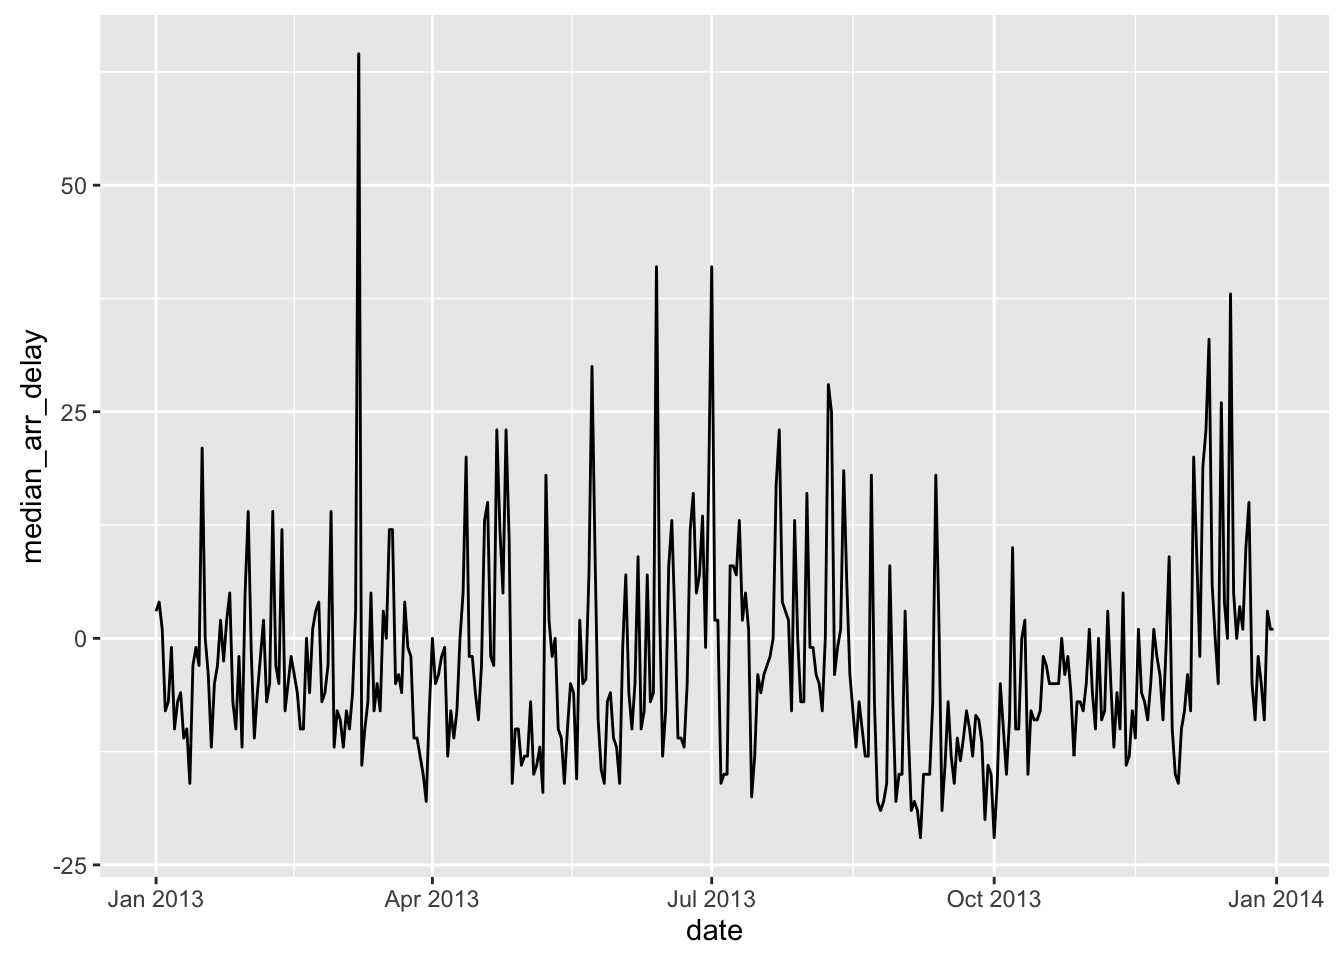
\includegraphics[width=\textwidth]{ismay_files/figure-latex/lineflights-1} 

}

\caption[Line-graph of median arrival delay for flights leaving NYC in 2013 versus day of the year]{Line-graph of median arrival delay for flights leaving NYC in 2013 versus day of the year}\label{fig:lineflights}
\end{figure}

\begin{center}\rule{0.5\linewidth}{\linethickness}\end{center}

\begin{learncheck}
\textbf{\emph{Learning check}}
\end{learncheck}

\textbf{(LC4.32)} Why should line-graphs be avoided when there is not a
clear ordering of the horizontal axis?

\textbf{(LC4.33)} Why are line-graphs frequently used when time is the
explanatory variable?

\textbf{(LC4.34)} Why did we use the \texttt{flights\_summarized}
dataframe to produce the line-graph in Figure \ref{fig:lineflights}
instead of \texttt{flights} or \texttt{flights\_day}?

\textbf{(LC4.35)} Are the largest median arrival delays where you
expected them to occur on the line-graph above in Figure
\ref{fig:lineflights}? Why or why not?

\begin{center}\rule{0.5\linewidth}{\linethickness}\end{center}

\subsection{Summary}\label{summary-4}

Line-graphs provide a useful tool for viewing a continuous variable that
is plotted versus time. We need to be careful to not be too entrenched
in using line-graphs whenever we wish though. They only make sense when
the explanatory variable (the one on the explanatory variable) has a
natural ordering. We can mislead our audience if that isn't the case.

\section{Brief Review of The Grammar of
Graphics}\label{brief-review-of-the-grammar-of-graphics}

The FNG discussion above has introduced you to all of the major pieces
behind ``The Grammar of Graphics'', which serves as the basis for the
\texttt{ggplot2} package. This theoretical framework given by Leland
Wilkinson \citep{wilkinson2005} helps us identify what the pieces are
that make up a statistical graphic:

\begin{quote}
In brief, the grammar tells us that a statistical graphic is a mapping
from data to aesthetic attributes (color, shape, size) of geometric
objects (points, lines, bars).
\end{quote}

Specially, we can break a graphic into the following components:

\begin{itemize}
\item
  \texttt{aes}: mappings of data to \emph{aesthetics} we can perceive on
  a graphic. These include x/y position, color, size, and shape. Each
  aesthetic can be mapped to a variable in our data set. If not
  assigned, they are set to defaults.
\item
  \texttt{geom}: (geometric objects) This refers to our type of plot:
  points, lines, bars, etc.
\item
  \texttt{stat}: (statistical transformations to summarize data) This
  includes smoothing, binning values into a histogram, or just itself
  \texttt{"identity"}. You'll see this when we get to regression later
  in Chapter \ref{regress}.
\item
  \texttt{facet}: how to break up data into subsets and display broken
  down plots as small multiples
\item
  \texttt{scales} both

  \begin{itemize}
  \tightlist
  \item
    convert \textbf{data units} to \textbf{physical units} the computer
    can display
  \item
    draw a legend and/or axes, which provide an inverse mapping to make
    it possible to read the original data values from the graph.
  \end{itemize}
\item
  \texttt{coord}: coordinate system for x/y values: typically cartesian.
\item
  \texttt{position} adjustments
\end{itemize}

There are other extra attributes that can be tweaked as well including
titles for the plot and each of the axes and also over-arching themes
for the plot. In general, the Grammar of Graphics allows for
customizability but also keeping with a consistent framework that allows
the user to easily tweak their creations as they wish or need to in
order to convey a message about their data.

We'll see (and have seen) that you don't necessarily need to include all
of these in your code to produce a plot but each of the components are
set by default and do exist with each plot produced using
\texttt{ggplot2}.

An excellent resource as you begin to create plots using the
\texttt{ggplot2} package is a cheatsheet that RStudio has put together
entitled ``Data Visualization with ggplot2'' available
\href{https://www.rstudio.com/wp-content/uploads/2015/12/ggplot2-cheatsheet-2.0.pdf}{here}.
This covers more than what we've discussed in this chapter but provides
nice visual descriptions of what each function produces.

\section{What's to come?}\label{whats-to-come-1}

In Chapter \ref{manip}, we'll further explore data by grouping our data,
creating summaries based on those groupings, filtering our data to match
conditions, selecting specific columns of our data, and other
manipulations with our data including defining new columns/variables.
These data manipulation procedures will go hand-in-hand with the data
visualizations you've produced here.

\chapter{Manipulating Data}\label{manip}

Let's briefly recap where we have been so far and where we are headed.
In Chapter \ref{tidy}, we discussed what it means for data to be tidy.
We saw that this corresponds to observations to correspond to rows and
for variables to be stored in columns. The entries in the data frame
correspond to different combinations of observational units and
variables. In the \texttt{flights} data frame, we saw that each row
corresponded to a different flight leaving New York City. (In other
words, the observational unit of that tidy data frame is a flight.) The
variables are listed as columns and for \texttt{flights} they include
both quantitative variables like \texttt{dep\_delay} and
\texttt{distance} but also categorical variables like \texttt{carrier}
and \texttt{origin}. An entry in the table corresponds to a particular
flight and a particular value of a given variable representing that
flight.

We saw in Chapter \ref{viz} that organizing data in this tidy way makes
it easy for use to produce graphics. We can simply specify what
variable/column we would like on one axis, what variable we'd like on
the other axis, and what type of plot we'd like to make. We can also do
things such as changing the color by another variable or change the size
of our points by a fourth variable given this tidy data set.

In Chapter \ref{viz}, we also introduced some ways to summarize and
manipulate data to suit your needs. This chapter focuses more on the
details of this by giving a variety of examples using the five main
verbs in the \texttt{dplyr} package. There are more advanced operations
that can be done than these and you'll see some examples of this near
the end of the chapter.

As we saw with the RStudio cheatsheet on
\href{https://www.rstudio.com/wp-content/uploads/2015/12/ggplot2-cheatsheet-2.0.pdf}{data
visualization}, RStudio has also created a cheatsheet for data
manipulation entitled ``Data Wrangling with dplyr and tidyr'' available
\href{https://www.rstudio.com/wp-content/uploads/2015/02/data-wrangling-cheatsheet.pdf}{here}.
We will focus only on the \texttt{dplyr} functions in this book, but you
are encouraged to also explore \texttt{tidyr} if you are presented with
data that is not in the tidy format that we have specified as the
preferred option for our purposes.

\section{Five Main Verbs - The FMV}\label{five-main-verbs---the-fmv}

If you scan over the Data Wrangling cheatsheet, you may be initially
overwhelmed by the amount of functions available. You'll see the use of
all of these as you work more and more with data frames in R. The
\texttt{d} in \texttt{dplyr} stands for data frames so the functions
here work when you are working with objects of the data frame type.

It's most important for you to focus on the five most commonly used
functions that help us manipulate and summarize data. A description of
these verbs follows with each subsection devoted to seeing an example of
that verb in play (or a combination of a few verbs):

\begin{itemize}
\tightlist
\item
  \texttt{select}: Choose variables/columns by their names
\item
  \texttt{filter}: Pick rows based on conditions about their values
\item
  \texttt{summarize}: Create summary measures of variables (or groups of
  observations on variables using \texttt{group\_by})
\item
  \texttt{mutate}: Make a new variable in the data frame
\item
  \texttt{arrange}: Sort the rows based on one or more variables
\end{itemize}

Just as we had the FNG (The Five Named Graphs in Chapter \ref{viz} using
\texttt{ggplot2}), we have the FMV here (The Five Main Verbs in
\texttt{dplyr}):

\subsection{\texorpdfstring{Select variables using
\texttt{select}}{Select variables using select}}\label{select-variables-using-select}

\begin{figure}

{\centering 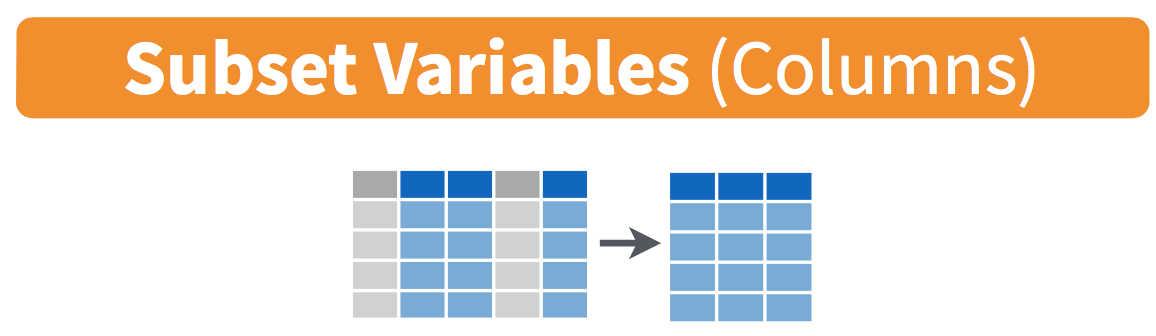
\includegraphics[width=\textwidth]{images/select} 

}

\caption[Select diagram from Data Wrangling with dplyr and tidyr cheatsheet]{Select diagram from Data Wrangling with dplyr and tidyr cheatsheet}\label{fig:selectfig}
\end{figure}

We've seen that the \texttt{flights} data frame in the
\texttt{nycflights13} package contains many different variables (19 in
fact). You can identify this by running the \texttt{dim} function:

\begin{Shaded}
\begin{Highlighting}[]
\KeywordTok{library}\NormalTok{(nycflights13)}
\KeywordTok{data}\NormalTok{(flights)}
\KeywordTok{dim}\NormalTok{(flights)}
\end{Highlighting}
\end{Shaded}

\begin{verbatim}
## [1] 336776     19
\end{verbatim}

One of these variables is \texttt{year}. If you remember the original
description of the \texttt{flights} data frame (or by running
\texttt{?flights}), you'll remember that this data correspond to flights
in 2013 departing New York City. The \texttt{year} variable isn't really
a variable here in that it doesn't vary\ldots{} \texttt{flights}
actually comes from a larger data set that covers many years. We may
want to remove the \texttt{year} variable from our data set. To do so
easily, we use the \texttt{select} variable:

\begin{Shaded}
\begin{Highlighting}[]
\KeywordTok{library}\NormalTok{(dplyr)}
\NormalTok{flights <-}\StringTok{ }\KeywordTok{select}\NormalTok{(}\DataTypeTok{.data =} \NormalTok{flights, -year)}
\KeywordTok{names}\NormalTok{(flights)}
\end{Highlighting}
\end{Shaded}

\begin{verbatim}
##  [1] "month"          "day"            "dep_time"       "sched_dep_time"
##  [5] "dep_delay"      "arr_time"       "sched_arr_time" "arr_delay"     
##  [9] "carrier"        "flight"         "tailnum"        "origin"        
## [13] "dest"           "air_time"       "distance"       "hour"          
## [17] "minute"         "time_hour"
\end{verbatim}

The \texttt{names} function gives a listing of all the columns in a data
frame. We see that \texttt{year} has been removed. This was done using a
\texttt{-} in front of the name of the column we'd like to remove.

We could also select specific columns (instead of deselecting columns)
by listing them out:

\begin{Shaded}
\begin{Highlighting}[]
\NormalTok{flight_dep_times <-}\StringTok{ }\KeywordTok{select}\NormalTok{(flights, month, day, dep_time, sched_dep_time)}
\NormalTok{flight_dep_times}
\end{Highlighting}
\end{Shaded}

\begin{verbatim}
## # A tibble: 336,776 x 4
##    month   day dep_time sched_dep_time
##    <int> <int>    <int>          <int>
## 1      1     1      517            515
## 2      1     1      533            529
## 3      1     1      542            540
## 4      1     1      544            545
## 5      1     1      554            600
## 6      1     1      554            558
## 7      1     1      555            600
## 8      1     1      557            600
## 9      1     1      557            600
## 10     1     1      558            600
## # ... with 336,766 more rows
\end{verbatim}

Or we could specify a ranges of columns:

\begin{Shaded}
\begin{Highlighting}[]
\NormalTok{flight_arr_times <-}\StringTok{ }\KeywordTok{select}\NormalTok{(flights, month:day, arr_time:sched_arr_time)}
\NormalTok{flight_arr_times}
\end{Highlighting}
\end{Shaded}

\begin{verbatim}
## # A tibble: 336,776 x 4
##    month   day arr_time sched_arr_time
##    <int> <int>    <int>          <int>
## 1      1     1      830            819
## 2      1     1      850            830
## 3      1     1      923            850
## 4      1     1     1004           1022
## 5      1     1      812            837
## 6      1     1      740            728
## 7      1     1      913            854
## 8      1     1      709            723
## 9      1     1      838            846
## 10     1     1      753            745
## # ... with 336,766 more rows
\end{verbatim}

The \texttt{select} function can also be used to reorder columns in
combination with the \texttt{everything} helper function. Let's suppose
we'd like the \texttt{hour}, \texttt{minute}, and \texttt{time\_hour}
variables, which appear at the end of the \texttt{flights} data set to
actually appear immediately after the \texttt{day} variable:

\begin{Shaded}
\begin{Highlighting}[]
\NormalTok{flights_reorder <-}\StringTok{ }\KeywordTok{select}\NormalTok{(flights, month:day, hour:time_hour, }\KeywordTok{everything}\NormalTok{())}
\KeywordTok{names}\NormalTok{(flights_reorder)}
\end{Highlighting}
\end{Shaded}

\begin{verbatim}
##  [1] "month"          "day"            "hour"           "minute"        
##  [5] "time_hour"      "dep_time"       "sched_dep_time" "dep_delay"     
##  [9] "arr_time"       "sched_arr_time" "arr_delay"      "carrier"       
## [13] "flight"         "tailnum"        "origin"         "dest"          
## [17] "air_time"       "distance"
\end{verbatim}

Lastly, the helper functions \texttt{starts\_with}, \texttt{ends\_with},
and \texttt{contains} can be used to choose column names that match
those conditions:

\begin{Shaded}
\begin{Highlighting}[]
\NormalTok{flights_begin_a <-}\StringTok{ }\KeywordTok{select}\NormalTok{(flights, }\KeywordTok{starts_with}\NormalTok{(}\StringTok{"a"}\NormalTok{))}
\NormalTok{flights_begin_a}
\end{Highlighting}
\end{Shaded}

\begin{verbatim}
## # A tibble: 336,776 x 3
##    arr_time arr_delay air_time
##       <int>     <dbl>    <dbl>
## 1       830        11      227
## 2       850        20      227
## 3       923        33      160
## 4      1004       -18      183
## 5       812       -25      116
## 6       740        12      150
## 7       913        19      158
## 8       709       -14       53
## 9       838        -8      140
## 10      753         8      138
## # ... with 336,766 more rows
\end{verbatim}

\begin{Shaded}
\begin{Highlighting}[]
\NormalTok{flights_delays <-}\StringTok{ }\KeywordTok{select}\NormalTok{(flights, }\KeywordTok{ends_with}\NormalTok{(}\StringTok{"delay"}\NormalTok{))}
\NormalTok{flights_delays}
\end{Highlighting}
\end{Shaded}

\begin{verbatim}
## # A tibble: 336,776 x 2
##    dep_delay arr_delay
##        <dbl>     <dbl>
## 1          2        11
## 2          4        20
## 3          2        33
## 4         -1       -18
## 5         -6       -25
## 6         -4        12
## 7         -5        19
## 8         -3       -14
## 9         -3        -8
## 10        -2         8
## # ... with 336,766 more rows
\end{verbatim}

\begin{Shaded}
\begin{Highlighting}[]
\NormalTok{flights_time <-}\StringTok{ }\KeywordTok{select}\NormalTok{(flights, }\KeywordTok{contains}\NormalTok{(}\StringTok{"time"}\NormalTok{))}
\NormalTok{flights_time}
\end{Highlighting}
\end{Shaded}

\begin{verbatim}
## # A tibble: 336,776 x 6
##    dep_time sched_dep_time arr_time sched_arr_time air_time
##       <int>          <int>    <int>          <int>    <dbl>
## 1       517            515      830            819      227
## 2       533            529      850            830      227
## 3       542            540      923            850      160
## 4       544            545     1004           1022      183
## 5       554            600      812            837      116
## 6       554            558      740            728      150
## 7       555            600      913            854      158
## 8       557            600      709            723       53
## 9       557            600      838            846      140
## 10      558            600      753            745      138
## # ... with 336,766 more rows, and 1 more variables: time_hour <time>
\end{verbatim}

Another useful function is \texttt{rename}, which as you may suspect
renames one column to another name. Suppose we wanted \texttt{dep\_time}
and \texttt{arr\_time} to be \texttt{departure\_time} and
\texttt{arrival\_time} instead in the \texttt{flights\_time} data frame:

\begin{Shaded}
\begin{Highlighting}[]
\NormalTok{flights_time <-}\StringTok{ }\KeywordTok{rename}\NormalTok{(flights_time,}
                       \DataTypeTok{departure_time =} \NormalTok{dep_time,}
                       \DataTypeTok{arrival_time =} \NormalTok{arr_time)}
\KeywordTok{names}\NormalTok{(flights_time)}
\end{Highlighting}
\end{Shaded}

\begin{verbatim}
## [1] "departure_time" "sched_dep_time" "arrival_time"   "sched_arr_time"
## [5] "air_time"       "time_hour"
\end{verbatim}

It's easy to forget if the new name comes before or after the equals
sign. I usually remember this as ``New Before, Old After'' or NBOA.

You'll receive an error if you try to do it the other way:

\begin{verbatim}
Error: Unknown variables: departure_time, arrival_time.
\end{verbatim}

\begin{center}\rule{0.5\linewidth}{\linethickness}\end{center}

\begin{learncheck}
\textbf{\emph{Learning check}}
\end{learncheck}

\textbf{(LC5.1)} How many different ways are there to select all three
of \texttt{dest}, \texttt{air\_time}, and \texttt{distance} variables
from \texttt{flights}? Give the code showing how to do all of them you
can think of.

\textbf{(LC5.2)} How could one use \texttt{starts\_with},
\texttt{ends\_with}, and \texttt{contains} to select columns from a
dataset with 100 or so columns? Think up a dataset that might have that
many columns and discuss how each of these functions could be used to
make smaller data sets.

\textbf{(LC5.3)} Why might we want to use the \texttt{select} function
on a data frame?

\begin{center}\rule{0.5\linewidth}{\linethickness}\end{center}

\subsection{\texorpdfstring{Filter observations using
\texttt{filter}}{Filter observations using filter}}\label{filter-observations-using-filter}

\begin{figure}

{\centering 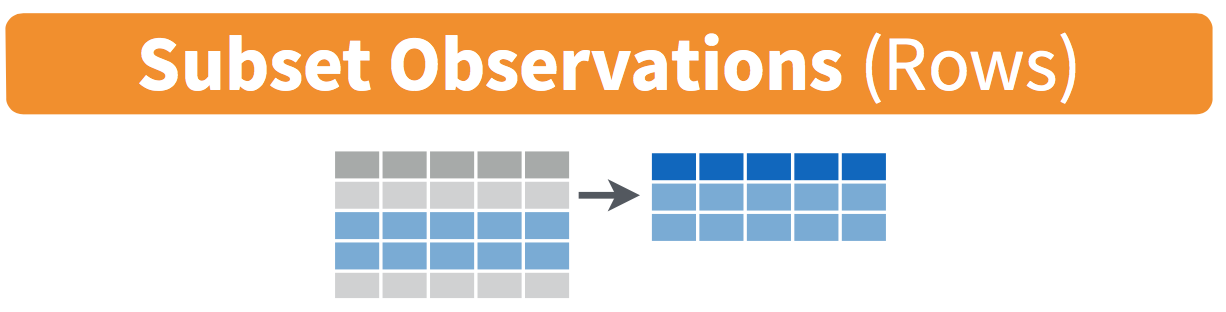
\includegraphics[width=\textwidth]{images/filter} 

}

\caption[Filter diagram from Data Wrangling with dplyr and tidyr cheatsheet]{Filter diagram from Data Wrangling with dplyr and tidyr cheatsheet}\label{fig:filter}
\end{figure}

All of the FMVs follow the same syntax with the first argument to the
function/verb being the name of the data frame and then the other
arguments specifying which criteria you'd like the verb to work with.

The \texttt{filter} function here works much like the ``Filter'' option
in Microsoft Excel. It allows you to specify criteria about values of
variable in your data set and then chooses only those rows that match
that criteria. We begin by focusing only on flights from New York City
to Portland, Oregon. The \texttt{dest} code (or airport code) for
Portland, Oregon is \texttt{"PDX"}:

\begin{Shaded}
\begin{Highlighting}[]
\NormalTok{portland_flights <-}\StringTok{ }\KeywordTok{filter}\NormalTok{(flights, dest ==}\StringTok{ "PDX"}\NormalTok{)}
\NormalTok{portland_flights}
\end{Highlighting}
\end{Shaded}

\begin{verbatim}
## # A tibble: 1,354 x 18
##    month   day dep_time sched_dep_time dep_delay arr_time
##    <int> <int>    <int>          <int>     <dbl>    <int>
## 1      1     1     1739           1740        -1     2051
## 2      1     1     1805           1757         8     2117
## 3      1     1     2052           2029        23     2349
## 4      1     2      804            805        -1     1039
## 5      1     2     1552           1550         2     1853
## 6      1     2     1727           1720         7     2042
## 7      1     2     1738           1740        -2     2028
## 8      1     2     2024           2029        -5     2314
## 9      1     3     1755           1745        10     2110
## 10     1     3     1814           1727        47     2108
## # ... with 1,344 more rows, and 12 more variables:
## #   sched_arr_time <int>, arr_delay <dbl>, carrier <chr>, flight <int>,
## #   tailnum <chr>, origin <chr>, dest <chr>, air_time <dbl>,
## #   distance <dbl>, hour <dbl>, minute <dbl>, time_hour <time>
\end{verbatim}

Note the second equals sign here. You are almost guaranteed to make the
mistake at least one of only including one equals sign. Let's see what
happens when we make this error:

\begin{Shaded}
\begin{Highlighting}[]
\NormalTok{portland_flights <-}\StringTok{ }\KeywordTok{filter}\NormalTok{(flights, }\DataTypeTok{dest =} \StringTok{"PDX"}\NormalTok{)}
\end{Highlighting}
\end{Shaded}

\begin{verbatim}
Error: filter() takes unnamed arguments. Do you need `==`?
\end{verbatim}

We see that there were 1354 flights from New York City to Portland in
2013. Let's combine this with what we saw in Subsection 5.1.1 to ensure
that Portland flights were selected:

\begin{Shaded}
\begin{Highlighting}[]
\NormalTok{reordered_flights <-}\StringTok{ }\KeywordTok{select}\NormalTok{(flights, dest, }\KeywordTok{everything}\NormalTok{())}
\NormalTok{pdx_flights <-}\StringTok{ }\KeywordTok{filter}\NormalTok{(reordered_flights, dest ==}\StringTok{ "PDX"}\NormalTok{)}
\NormalTok{pdx_flights}
\end{Highlighting}
\end{Shaded}

\begin{verbatim}
## # A tibble: 1,354 x 18
##     dest month   day dep_time sched_dep_time dep_delay arr_time
##    <chr> <int> <int>    <int>          <int>     <dbl>    <int>
## 1    PDX     1     1     1739           1740        -1     2051
## 2    PDX     1     1     1805           1757         8     2117
## 3    PDX     1     1     2052           2029        23     2349
## 4    PDX     1     2      804            805        -1     1039
## 5    PDX     1     2     1552           1550         2     1853
## 6    PDX     1     2     1727           1720         7     2042
## 7    PDX     1     2     1738           1740        -2     2028
## 8    PDX     1     2     2024           2029        -5     2314
## 9    PDX     1     3     1755           1745        10     2110
## 10   PDX     1     3     1814           1727        47     2108
## # ... with 1,344 more rows, and 11 more variables:
## #   sched_arr_time <int>, arr_delay <dbl>, carrier <chr>, flight <int>,
## #   tailnum <chr>, origin <chr>, air_time <dbl>, distance <dbl>,
## #   hour <dbl>, minute <dbl>, time_hour <time>
\end{verbatim}

We see that Portland flights were selected here. You could also run
\texttt{View(pdx\_flights)} to glance at the data in spreadsheet form.

You can combine multiple criteria together using operators that make
comparisons:

\begin{itemize}
\tightlist
\item
  \texttt{\textbar{}} corresponds to ``or''
\item
  \texttt{\&} corresponds to ``and''
\end{itemize}

We can often skip the use of \texttt{\&} and just separate our
conditions with a comma. You'll see this in the example below.

In addition, you can use other mathematical checks (similar to
\texttt{==}):

\begin{itemize}
\tightlist
\item
  \texttt{\textgreater{}} corresponds to ``greater than''
\item
  \texttt{\textless{}} corresponds to ``less than''
\item
  \texttt{\textgreater{}=} corresponds to ``greater than or equal to''
\item
  \texttt{\textless{}=} corresponds to ``less than or equal to''
\item
  \texttt{!=} corresponds to ``not equal to''
\end{itemize}

To see many of these in action, let's select all flights that left JFK
airport heading to Burlington, Vermont (\texttt{"BTV"}) or Seattle,
Washington (\texttt{"SEA"}) in the months of October, November, or
December:

\begin{Shaded}
\begin{Highlighting}[]
\NormalTok{btv_sea_flights_fall <-}\StringTok{ }\KeywordTok{filter}\NormalTok{(flights,}
                               \NormalTok{origin ==}\StringTok{ "JFK"}\NormalTok{, }
                               \NormalTok{(dest ==}\StringTok{ "BTV"}\NormalTok{) |}\StringTok{ }\NormalTok{(dest ==}\StringTok{ "SEA"}\NormalTok{),}
                               \NormalTok{month >=}\StringTok{ }\DecValTok{10}\NormalTok{)}
\end{Highlighting}
\end{Shaded}

Another example uses the \texttt{!} to choose pick rows that
\textbf{DON'T} match a condition. Here we are referring to excluding the
Northern Hemisphere summer months of June, July, and August.

\begin{Shaded}
\begin{Highlighting}[]
\NormalTok{not_summer_flights <-}\StringTok{ }\KeywordTok{filter}\NormalTok{(flights,}
                             \NormalTok{!}\KeywordTok{between}\NormalTok{(month, }\DecValTok{6}\NormalTok{, }\DecValTok{8}\NormalTok{))}
\NormalTok{not_summer_flights}
\end{Highlighting}
\end{Shaded}

\begin{verbatim}
## # A tibble: 249,781 x 18
##    month   day dep_time sched_dep_time dep_delay arr_time
##    <int> <int>    <int>          <int>     <dbl>    <int>
## 1      1     1      517            515         2      830
## 2      1     1      533            529         4      850
## 3      1     1      542            540         2      923
## 4      1     1      544            545        -1     1004
## 5      1     1      554            600        -6      812
## 6      1     1      554            558        -4      740
## 7      1     1      555            600        -5      913
## 8      1     1      557            600        -3      709
## 9      1     1      557            600        -3      838
## 10     1     1      558            600        -2      753
## # ... with 249,771 more rows, and 12 more variables:
## #   sched_arr_time <int>, arr_delay <dbl>, carrier <chr>, flight <int>,
## #   tailnum <chr>, origin <chr>, dest <chr>, air_time <dbl>,
## #   distance <dbl>, hour <dbl>, minute <dbl>, time_hour <time>
\end{verbatim}

To check that we are correct here we can use the \texttt{count} function
on the \texttt{month} variable in our \texttt{not\_summer\_flights} data
frame to ensure June, July, and August are not selected:

\begin{Shaded}
\begin{Highlighting}[]
\KeywordTok{count}\NormalTok{(not_summer_flights, month)}
\end{Highlighting}
\end{Shaded}

\begin{verbatim}
## # A tibble: 9 x 2
##   month     n
##   <int> <int>
## 1     1 27004
## 2     2 24951
## 3     3 28834
## 4     4 28330
## 5     5 28796
## 6     9 27574
## 7    10 28889
## 8    11 27268
## 9    12 28135
\end{verbatim}

The function \texttt{between} is a shortcut. We could also have written
the following to get the same result:

\begin{Shaded}
\begin{Highlighting}[]
\NormalTok{not_summer2 <-}\StringTok{ }\KeywordTok{filter}\NormalTok{(flights, month <=}\StringTok{ }\DecValTok{5} \NormalTok{|}\StringTok{ }\NormalTok{month >=}\StringTok{ }\DecValTok{9}\NormalTok{)}
\KeywordTok{count}\NormalTok{(not_summer2, month)}
\end{Highlighting}
\end{Shaded}

\begin{verbatim}
## # A tibble: 9 x 2
##   month     n
##   <int> <int>
## 1     1 27004
## 2     2 24951
## 3     3 28834
## 4     4 28330
## 5     5 28796
## 6     9 27574
## 7    10 28889
## 8    11 27268
## 9    12 28135
\end{verbatim}

\begin{learncheck}
\textbf{\emph{Learning check}}
\end{learncheck}

\textbf{(LC5.4)} What's another way using \texttt{!} we could filter
only the rows that are not summer months (June, July, or August) in the
\texttt{flights} data frame?

\begin{center}\rule{0.5\linewidth}{\linethickness}\end{center}

\subsection{\texorpdfstring{Summarize variables using
\texttt{summarize}}{Summarize variables using summarize}}\label{summarize-variables-using-summarize}

\begin{figure}

{\centering 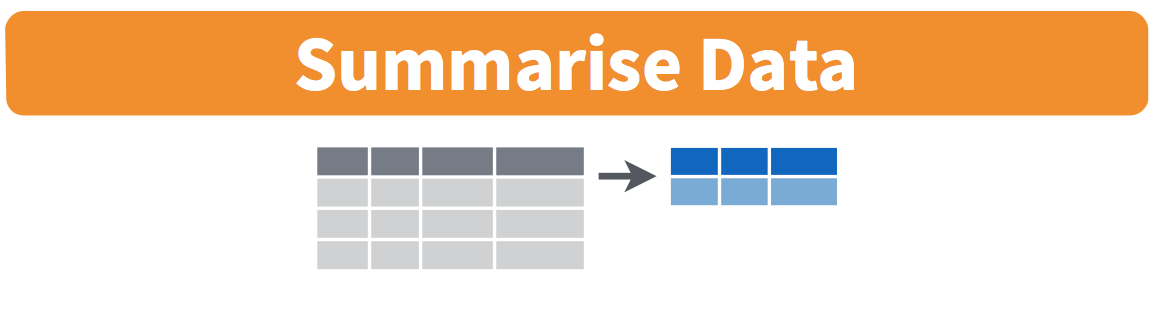
\includegraphics[width=\textwidth]{images/summarize1} 

}

\caption[Summarize diagram from Data Wrangling with dplyr and tidyr cheatsheet]{Summarize diagram from Data Wrangling with dplyr and tidyr cheatsheet}\label{fig:sum1}
\end{figure}

\begin{figure}

{\centering 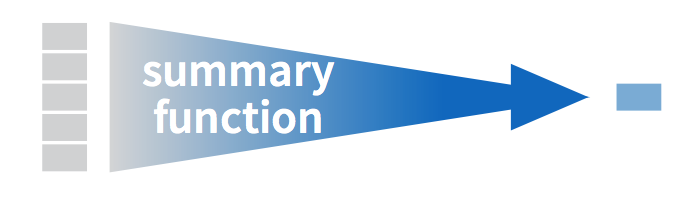
\includegraphics[width=\textwidth]{images/summary} 

}

\caption[Another summarize diagram from Data Wrangling with dplyr and tidyr cheatsheet]{Another summarize diagram from Data Wrangling with dplyr and tidyr cheatsheet}\label{fig:sum2}
\end{figure}

We saw in Subsection \ref{contsum} a way to calculate the standard
deviation and mean of the temperature variable \texttt{temp} in the
\texttt{weather} data frame of \texttt{nycflights}. We can do so in one
step using the \texttt{summarize} function in \texttt{dplyr}:

\begin{Shaded}
\begin{Highlighting}[]
\KeywordTok{summarize}\NormalTok{(weather,}
          \DataTypeTok{mean =} \KeywordTok{mean}\NormalTok{(temp),}
          \DataTypeTok{std_dev =} \KeywordTok{sd}\NormalTok{(temp))}
\end{Highlighting}
\end{Shaded}

\begin{verbatim}
## # A tibble: 1 x 2
##    mean std_dev
##   <dbl>   <dbl>
## 1    NA      NA
\end{verbatim}

What happened here? The mean and the standard deviation temperatures are
missing? Remember that by default the \texttt{mean} and \texttt{sd}
functions do not ignore missing values. We need to specify \texttt{TRUE}
for the \texttt{na.rm} parameter:

\begin{Shaded}
\begin{Highlighting}[]
\NormalTok{summary_temp <-}\StringTok{ }\KeywordTok{summarize}\NormalTok{(weather,}
          \DataTypeTok{mean =} \KeywordTok{mean}\NormalTok{(temp, }\DataTypeTok{na.rm =} \OtherTok{TRUE}\NormalTok{),}
          \DataTypeTok{std_dev =} \KeywordTok{sd}\NormalTok{(temp, }\DataTypeTok{na.rm =} \OtherTok{TRUE}\NormalTok{)}
          \NormalTok{)}
\NormalTok{summary_temp}
\end{Highlighting}
\end{Shaded}

\begin{verbatim}
## # A tibble: 1 x 2
##       mean  std_dev
##      <dbl>    <dbl>
## 1 55.20351 17.78212
\end{verbatim}

We've created a small data frame here called \texttt{summary\_temp} that
includes both the \texttt{mean} and the \texttt{std\_dev} of the
\texttt{temp} variable in \texttt{weather}. If we'd like to access
either of these values directly we can use the \texttt{\$} to specify a
column in a data frame:

\begin{Shaded}
\begin{Highlighting}[]
\NormalTok{summary_temp$mean}
\end{Highlighting}
\end{Shaded}

\begin{verbatim}
## [1] 55.20351
\end{verbatim}

\begin{Shaded}
\begin{Highlighting}[]
\NormalTok{summary_temp$std_dev}
\end{Highlighting}
\end{Shaded}

\begin{verbatim}
## [1] 17.78212
\end{verbatim}

It's often more useful to summarize a variable based on the groupings of
another variable. Let's say we were interested in the mean and standard
deviation of temperatures for each month. We believe that you will be
amazed at just how simple this is:

\begin{figure}

{\centering 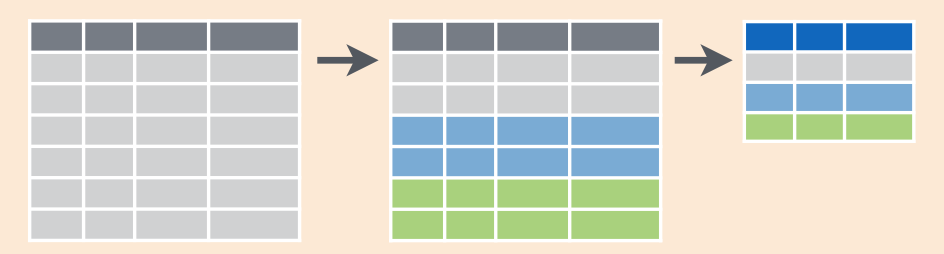
\includegraphics[width=\textwidth]{images/group_summary} 

}

\caption[Group by and summarize diagram from Data Wrangling with dplyr and tidyr cheatsheet]{Group by and summarize diagram from Data Wrangling with dplyr and tidyr cheatsheet}\label{fig:groupsummarize}
\end{figure}

\begin{Shaded}
\begin{Highlighting}[]
\NormalTok{grouped_weather <-}\StringTok{ }\KeywordTok{group_by}\NormalTok{(weather, month)}
\NormalTok{summary_tempXmonth <-}\StringTok{ }\KeywordTok{summarize}\NormalTok{(grouped_weather,}
          \DataTypeTok{mean =} \KeywordTok{mean}\NormalTok{(temp, }\DataTypeTok{na.rm =} \OtherTok{TRUE}\NormalTok{),}
          \DataTypeTok{std_dev =} \KeywordTok{sd}\NormalTok{(temp, }\DataTypeTok{na.rm =} \OtherTok{TRUE}\NormalTok{)}
          \NormalTok{)}
\NormalTok{summary_tempXmonth}
\end{Highlighting}
\end{Shaded}

\begin{verbatim}
## # A tibble: 12 x 3
##    month     mean   std_dev
##    <dbl>    <dbl>     <dbl>
## 1      1 35.64127 10.185459
## 2      2 34.15454  6.940228
## 3      3 39.81404  6.224948
## 4      4 51.67094  8.785250
## 5      5 61.59185  9.608687
## 6      6 72.14500  7.603356
## 7      7 80.00967  7.147631
## 8      8 74.40495  5.171365
## 9      9 67.42582  8.475824
## 10    10 60.03305  8.829652
## 11    11 45.10893 10.502249
## 12    12 38.36811  9.940822
\end{verbatim}

By simply grouping the \texttt{weather} data set by \texttt{month} first
and then passing this new data frame into \texttt{summarize} we get a
resulting data frame that shows the mean and standard deviation
temperature for each month in New York City.

Another useful function is the \texttt{n} function which gives a count
of how many entries appeared in the groupings. Suppose we'd like to get
a sense for how many flights departed each of the three airports in New
York City:

\begin{Shaded}
\begin{Highlighting}[]
\NormalTok{grouped_flights <-}\StringTok{ }\KeywordTok{group_by}\NormalTok{(flights, origin)}
\NormalTok{by_origin <-}\StringTok{ }\KeywordTok{summarize}\NormalTok{(grouped_flights,}
                       \DataTypeTok{count =} \KeywordTok{n}\NormalTok{())}
\NormalTok{by_origin}
\end{Highlighting}
\end{Shaded}

\begin{verbatim}
## # A tibble: 3 x 2
##   origin  count
##    <chr>  <int>
## 1    EWR 120835
## 2    JFK 111279
## 3    LGA 104662
\end{verbatim}

We see that Newark (\texttt{"EWR"}) had the most flights departing in
2013 followed by \texttt{"JFK"} and lastly by LaGuardia
(\texttt{"LGA"}).

\begin{learncheck}
\textbf{\emph{Learning check}}
\end{learncheck}

\textbf{(LC5.5)} What does the standard deviation column in the
\texttt{summary\_tempXmonth} data frame tell us about temperatures in
New York City throughout the year?

\textbf{(LC5.6)} What code would be required to get the mean and
standard deviation temperature for each day in 2013 for NYC?

\textbf{(LC5.7)} How could we identify how many flights left each of the
three airports in each of the months of 2013?

\begin{center}\rule{0.5\linewidth}{\linethickness}\end{center}

\subsection{\texorpdfstring{Create new variables/change old variables
using
\texttt{mutate}}{Create new variables/change old variables using mutate}}\label{create-new-variableschange-old-variables-using-mutate}

\begin{figure}

{\centering 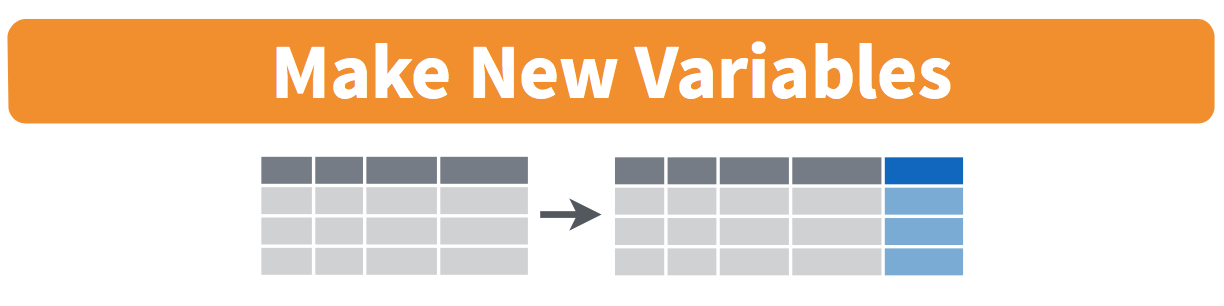
\includegraphics[width=\textwidth]{images/mutate} 

}

\caption[Mutate diagram from Data Wrangling with dplyr and tidyr cheatsheet]{Mutate diagram from Data Wrangling with dplyr and tidyr cheatsheet}\label{fig:select}
\end{figure}

When looking at the \texttt{flights} data set, there are some clear
additional variables that could be calculated based on the values of
variables already in the data set. Passengers are often frustrated when
their flights departs late, but change their mood a bit if pilots can
make up some time during the flight to get them to their destination
close to when they expected to land. This is commonly referred to as
gain and we will create this variable using the \texttt{mutate}
function:

\begin{Shaded}
\begin{Highlighting}[]
\NormalTok{flights_plus <-}\StringTok{ }\KeywordTok{mutate}\NormalTok{(flights,}
         \DataTypeTok{gain =} \NormalTok{arr_delay -}\StringTok{ }\NormalTok{dep_delay)}
\end{Highlighting}
\end{Shaded}

We can now look at summary measures of this \texttt{gain} variable and
even plot it in the form of a histogram:

\begin{Shaded}
\begin{Highlighting}[]
\NormalTok{gain_summary <-}\StringTok{ }\KeywordTok{summarize}\NormalTok{(flights_plus,}
          \DataTypeTok{min =} \KeywordTok{min}\NormalTok{(gain, }\DataTypeTok{na.rm =} \OtherTok{TRUE}\NormalTok{),}
          \DataTypeTok{q1 =} \KeywordTok{quantile}\NormalTok{(gain, }\FloatTok{0.25}\NormalTok{, }\DataTypeTok{na.rm =} \OtherTok{TRUE}\NormalTok{),}
          \DataTypeTok{median =} \KeywordTok{quantile}\NormalTok{(gain, }\FloatTok{0.5}\NormalTok{, }\DataTypeTok{na.rm =} \OtherTok{TRUE}\NormalTok{),}
          \DataTypeTok{q3 =} \KeywordTok{quantile}\NormalTok{(gain, }\FloatTok{0.75}\NormalTok{, }\DataTypeTok{na.rm =} \OtherTok{TRUE}\NormalTok{),}
          \DataTypeTok{max =} \KeywordTok{max}\NormalTok{(gain, }\DataTypeTok{na.rm =} \OtherTok{TRUE}\NormalTok{),}
          \DataTypeTok{mean =} \KeywordTok{mean}\NormalTok{(gain, }\DataTypeTok{na.rm =} \OtherTok{TRUE}\NormalTok{),}
          \DataTypeTok{sd =} \KeywordTok{sd}\NormalTok{(gain, }\DataTypeTok{na.rm =} \OtherTok{TRUE}\NormalTok{),}
          \DataTypeTok{missing =} \KeywordTok{sum}\NormalTok{(}\KeywordTok{is.na}\NormalTok{(gain))}
\NormalTok{)}
\NormalTok{gain_summary}
\end{Highlighting}
\end{Shaded}

\begin{verbatim}
## # A tibble: 1 x 8
##     min    q1 median    q3   max      mean       sd missing
##   <dbl> <dbl>  <dbl> <dbl> <dbl>     <dbl>    <dbl>   <int>
## 1  -109   -17     -7     3   196 -5.659779 18.04365    9430
\end{verbatim}

We've recreated the \texttt{summary} function we say in Chapter
\ref{viz} here using the \texttt{summarize} function in \texttt{dplyr}.

\begin{Shaded}
\begin{Highlighting}[]
\KeywordTok{library}\NormalTok{(ggplot2)}
\KeywordTok{ggplot}\NormalTok{(flights_plus, }\KeywordTok{aes}\NormalTok{(}\DataTypeTok{x =} \NormalTok{gain)) +}
\StringTok{  }\KeywordTok{geom_histogram}\NormalTok{(}\DataTypeTok{color =} \StringTok{"white"}\NormalTok{, }\DataTypeTok{bins =} \DecValTok{20}\NormalTok{)}
\end{Highlighting}
\end{Shaded}

\begin{figure}

{\centering 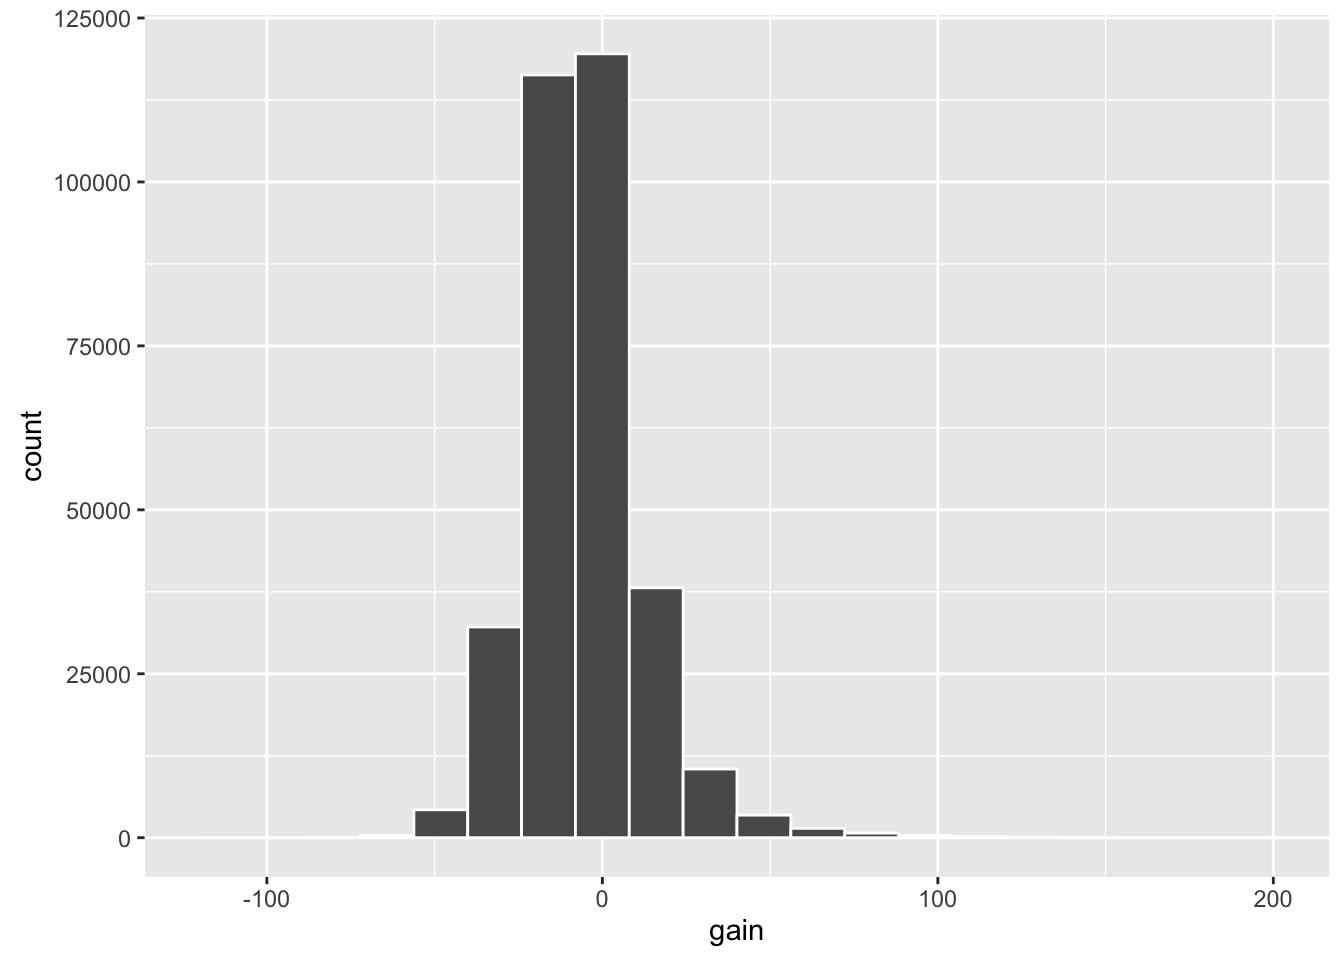
\includegraphics[width=\textwidth]{ismay_files/figure-latex/unnamed-chunk-58-1} 

}

\caption[Histogram of gain variable]{Histogram of gain variable}\label{fig:unnamed-chunk-58}
\end{figure}

We can also create multiple columns at once and even refer to columns
that were just created in a new column. Hadley produces one such example
in Chapter 5 of ``R for Data Science'' \citep{rds2016}:

\begin{Shaded}
\begin{Highlighting}[]
\NormalTok{flights_plus2 <-}\StringTok{ }\KeywordTok{mutate}\NormalTok{(flights,}
  \DataTypeTok{gain =} \NormalTok{arr_delay -}\StringTok{ }\NormalTok{dep_delay,}
  \DataTypeTok{hours =} \NormalTok{air_time /}\StringTok{ }\DecValTok{60}\NormalTok{,}
  \DataTypeTok{gain_per_hour =} \NormalTok{gain /}\StringTok{ }\NormalTok{hours}
\NormalTok{)}
\end{Highlighting}
\end{Shaded}

\begin{center}\rule{0.5\linewidth}{\linethickness}\end{center}

\begin{learncheck}
\textbf{\emph{Learning check}}
\end{learncheck}

\textbf{(LC5.8)} What do positive values of the \texttt{gain} variable
in \texttt{flights\_plus} correspond to? What about negative values? And
what about a zero value?

\textbf{(LC5.9)} Could we create the \texttt{dep\_delay} and
\texttt{arr\_delay} columns by simply subtracting \texttt{dep\_time}
from \texttt{sched\_dep\_time} and similarly for arrivals? Try the code
out and explain any differences between the result and what actually
appears in \texttt{flights}.

\textbf{(LC5.10)} What can we say about the distribution of
\texttt{gain}? Describe it in a few sentences using the plot and the
\texttt{gain\_summary} data frame values.

\begin{center}\rule{0.5\linewidth}{\linethickness}\end{center}

\subsection{\texorpdfstring{Reorder the data frame using
\texttt{arrange}}{Reorder the data frame using arrange}}\label{reorder-the-data-frame-using-arrange}

If you've ever worked with data, one of the most common things you'd
like to do is sort it. Have you ever been asked to calculate a median by
hand? This requires you to put the data in order from smallest to
highest in value. The \texttt{dplyr} package has a function called
\texttt{arrange} that we will use to sort/reorder our data according to
the values of the specified variable. This is most frequently used after
we have used the \texttt{group\_by} and \texttt{summarize} functions as
we will see.

Let's suppose we were interested in determining the most frequent
destination airports from New York City in 2013:

\begin{Shaded}
\begin{Highlighting}[]
\NormalTok{by_dest <-}\StringTok{ }\KeywordTok{group_by}\NormalTok{(flights, dest)}
\NormalTok{freq_dest <-}\StringTok{ }\KeywordTok{summarize}\NormalTok{(by_dest, }\DataTypeTok{num_flights =} \KeywordTok{n}\NormalTok{())}
\NormalTok{freq_dest}
\end{Highlighting}
\end{Shaded}

\begin{verbatim}
## # A tibble: 105 x 2
##     dest num_flights
##    <chr>       <int>
## 1    ABQ         254
## 2    ACK         265
## 3    ALB         439
## 4    ANC           8
## 5    ATL       17215
## 6    AUS        2439
## 7    AVL         275
## 8    BDL         443
## 9    BGR         375
## 10   BHM         297
## # ... with 95 more rows
\end{verbatim}

You'll see that by default the values of \texttt{dest} are displayed in
alphabetical order here. Remember to use \texttt{View()} in the R
Console to look at all the values of \texttt{freq\_dest} in spreadsheet
format. We are interested in finding those airports that appear most:

\begin{Shaded}
\begin{Highlighting}[]
\KeywordTok{arrange}\NormalTok{(freq_dest, num_flights)}
\end{Highlighting}
\end{Shaded}

\begin{verbatim}
## # A tibble: 105 x 2
##     dest num_flights
##    <chr>       <int>
## 1    LEX           1
## 2    LGA           1
## 3    ANC           8
## 4    SBN          10
## 5    HDN          15
## 6    MTJ          15
## 7    EYW          17
## 8    PSP          19
## 9    JAC          25
## 10   BZN          36
## # ... with 95 more rows
\end{verbatim}

This is actually giving us the opposite of what we are looking for. It
tells us the least frequent destination airports. To switch the ordering
to be descending instead of ascending we use the \texttt{desc} function:

\begin{Shaded}
\begin{Highlighting}[]
\KeywordTok{arrange}\NormalTok{(freq_dest, }\KeywordTok{desc}\NormalTok{(num_flights))}
\end{Highlighting}
\end{Shaded}

\begin{verbatim}
## # A tibble: 105 x 2
##     dest num_flights
##    <chr>       <int>
## 1    ORD       17283
## 2    ATL       17215
## 3    LAX       16174
## 4    BOS       15508
## 5    MCO       14082
## 6    CLT       14064
## 7    SFO       13331
## 8    FLL       12055
## 9    MIA       11728
## 10   DCA        9705
## # ... with 95 more rows
\end{verbatim}

We can also use the \texttt{top\_n} function which automatically tells
us the most frequent \texttt{num\_flights}. We specify the top 10
airports here:

\begin{Shaded}
\begin{Highlighting}[]
\KeywordTok{top_n}\NormalTok{(freq_dest, }\DataTypeTok{n =} \DecValTok{10}\NormalTok{, }\DataTypeTok{wt =} \NormalTok{num_flights)}
\end{Highlighting}
\end{Shaded}

\begin{verbatim}
## # A tibble: 10 x 2
##     dest num_flights
##    <chr>       <int>
## 1    ATL       17215
## 2    BOS       15508
## 3    CLT       14064
## 4    DCA        9705
## 5    FLL       12055
## 6    LAX       16174
## 7    MCO       14082
## 8    MIA       11728
## 9    ORD       17283
## 10   SFO       13331
\end{verbatim}

We'll still need to arrange this by \texttt{num\_flights} though:

\begin{Shaded}
\begin{Highlighting}[]
\KeywordTok{arrange}\NormalTok{(}\KeywordTok{top_n}\NormalTok{(freq_dest, }\DataTypeTok{n =} \DecValTok{10}\NormalTok{, }\DataTypeTok{wt =} \NormalTok{num_flights), }\KeywordTok{desc}\NormalTok{(num_flights))}
\end{Highlighting}
\end{Shaded}

\begin{verbatim}
## # A tibble: 10 x 2
##     dest num_flights
##    <chr>       <int>
## 1    ORD       17283
## 2    ATL       17215
## 3    LAX       16174
## 4    BOS       15508
## 5    MCO       14082
## 6    CLT       14064
## 7    SFO       13331
## 8    FLL       12055
## 9    MIA       11728
## 10   DCA        9705
\end{verbatim}

\textbf{Note:} Remember that I didn't pull the \texttt{n} and
\texttt{wt} arguments out of thin air. They can be found by using the
\texttt{?} function on \texttt{top\_n}.

\begin{learncheck}
\textbf{\emph{Learning check}}
\end{learncheck}

\textbf{(LC5.11)} Create a new data frame that shows the top 5 airports
with the largest arrival delays from NYC in 2013.

\begin{center}\rule{0.5\linewidth}{\linethickness}\end{center}

\section{\texorpdfstring{The pipe
\texttt{\%\textgreater{}\%}}{The pipe \%\textgreater{}\%}}\label{the-pipe}

Just as the \texttt{+} sign was used to add layers to a plot created
using \texttt{ggplot} we will use the pipe operator
(\texttt{\%\textgreater{}\%}) to chain together \texttt{dplyr}
functions. We'll see that we can even chain together \texttt{dplyr}
functions and plotting code. (Both \texttt{ggplot2} and \texttt{dplyr}
were created by Hadley after all.)

You may have been a little confused by the last chunk we created above:

\begin{Shaded}
\begin{Highlighting}[]
\KeywordTok{arrange}\NormalTok{(}\KeywordTok{top_n}\NormalTok{(freq_dest, }\DataTypeTok{n =} \DecValTok{10}\NormalTok{, }\DataTypeTok{wt =} \NormalTok{num_flights), }\KeywordTok{desc}\NormalTok{(num_flights))}
\end{Highlighting}
\end{Shaded}

If we don't create temporary variables like we did before with
\texttt{by\_dest}, \texttt{grouped\_flights}, etc., we start to get into
the issue of trying to match parentheses. We could separate this code a
bit to help with this:

\begin{Shaded}
\begin{Highlighting}[]
\KeywordTok{arrange}\NormalTok{(}
  \KeywordTok{top_n}\NormalTok{(freq_dest, }
        \DataTypeTok{n =} \DecValTok{10}\NormalTok{,}
        \DataTypeTok{wt =} \NormalTok{num_flights), }
  \KeywordTok{desc}\NormalTok{(num_flights))}
\end{Highlighting}
\end{Shaded}

\begin{verbatim}
## # A tibble: 10 x 2
##     dest num_flights
##    <chr>       <int>
## 1    ORD       17283
## 2    ATL       17215
## 3    LAX       16174
## 4    BOS       15508
## 5    MCO       14082
## 6    CLT       14064
## 7    SFO       13331
## 8    FLL       12055
## 9    MIA       11728
## 10   DCA        9705
\end{verbatim}

Even this make it difficult to understand what is exactly happening
though. \texttt{desc(num\_flights)} is an argument to \texttt{arrange}.
The best way to fix this problem is the use of the chaining operator
called the pipe (\texttt{\%\textgreater{}\%}):

\begin{Shaded}
\begin{Highlighting}[]
\NormalTok{freq_dest %>%}
\StringTok{  }\KeywordTok{top_n}\NormalTok{(}\DataTypeTok{n =} \DecValTok{10}\NormalTok{, }\DataTypeTok{wt =} \NormalTok{num_flights) %>%}
\StringTok{  }\KeywordTok{arrange}\NormalTok{(}\KeywordTok{desc}\NormalTok{(num_flights))}
\end{Highlighting}
\end{Shaded}

\begin{verbatim}
## # A tibble: 10 x 2
##     dest num_flights
##    <chr>       <int>
## 1    ORD       17283
## 2    ATL       17215
## 3    LAX       16174
## 4    BOS       15508
## 5    MCO       14082
## 6    CLT       14064
## 7    SFO       13331
## 8    FLL       12055
## 9    MIA       11728
## 10   DCA        9705
\end{verbatim}

Recall from Chapter \ref{viz} that we read the pipe operator as ``and
then''. So here we take the \texttt{freq\_dest} data frame \textbf{AND
THEN} we determine the top 10 values of \texttt{num\_flights}
\textbf{AND THEN} we arrange these top 10 flights according to a
descending numbers of flights (from highest to lowest).

We can go one stop further and tie together the \texttt{group\_by} and
\texttt{summarize} functions we used to find the most frequent flights:

\begin{Shaded}
\begin{Highlighting}[]
\NormalTok{ten_freq_dests <-}\StringTok{ }\NormalTok{flights %>%}
\StringTok{  }\KeywordTok{group_by}\NormalTok{(dest) %>%}
\StringTok{  }\KeywordTok{summarize}\NormalTok{(}\DataTypeTok{num_flights =} \KeywordTok{n}\NormalTok{()) %>%}
\StringTok{  }\KeywordTok{top_n}\NormalTok{(}\DataTypeTok{n =} \DecValTok{10}\NormalTok{) %>%}
\StringTok{  }\KeywordTok{arrange}\NormalTok{(}\KeywordTok{desc}\NormalTok{(num_flights))}
\end{Highlighting}
\end{Shaded}

\begin{verbatim}
## Selecting by num_flights
\end{verbatim}

\begin{learncheck}
\textbf{\emph{Learning check}}
\end{learncheck}

\textbf{(LC5.12)} Recreate each of the chunks of code above Subsection
5.1.5 in this chapter using the \texttt{\%\textgreater{}\%} operator.
Note that sometimes you can combine multiple subsequent chunks of code
together. Do so whenever possible.

\textbf{(LC5.13)} What benefits can you see to using the pipe instead of
the other way of doing things as you saw throughout this chapter? Give
specific examples.

\textbf{(LC5.14)} Write out exactly how the \texttt{ten\_freq\_dests}
data set was created using the ``and then'' verbiage.

\begin{center}\rule{0.5\linewidth}{\linethickness}\end{center}

The piping syntax will be our major focus throughout the rest of this
book and you'll find that you'll quickly be addicted to the chaining
with some practice. If you'd like to see more examples on using
\texttt{dplyr}, the FMV (in addition to some other \texttt{dplyr}
verbs), and \texttt{\%\textgreater{}\%} with the \texttt{nycflights13}
data set, you can check out Chapter 5 of Hadley and Garrett's book
\citep{rds2016}.

\section{Joining/merging data frames}\label{joiningmerging-data-frames}

Something you may have thought to yourself as you looked at the most
freqent destinations of flights from NYC in 2013 is

\begin{itemize}
\tightlist
\item
  ``What cities are these airports in?''
\item
  ``Is \texttt{"ORD"} Orlando?''
\item
  ``Where is \texttt{"FLL"}?
\end{itemize}

The \texttt{nycflights13} data source contains multiple data frames.
Instead of having to manually look up different values of airport names
corresponding to airport codes like \texttt{ORD}, we can have R
automatically do this ``looking up'' for us.

To do so, we'll need to tell R how to match one data frame to another
data frame. Let's first check out the \texttt{airports} data frame
inside of R:

\begin{Shaded}
\begin{Highlighting}[]
\KeywordTok{View}\NormalTok{(airports)}
\end{Highlighting}
\end{Shaded}

The first column \texttt{faa} corresponds to the airport codes that we
saw in \texttt{dest} in our \texttt{flights} and subsequent
\texttt{ten\_freq\_dests} data sets. Hadley and Garrett \citep{rds2016}
created the following diagram to help us understand how the different
data sets are linked:

\begin{figure}

{\centering 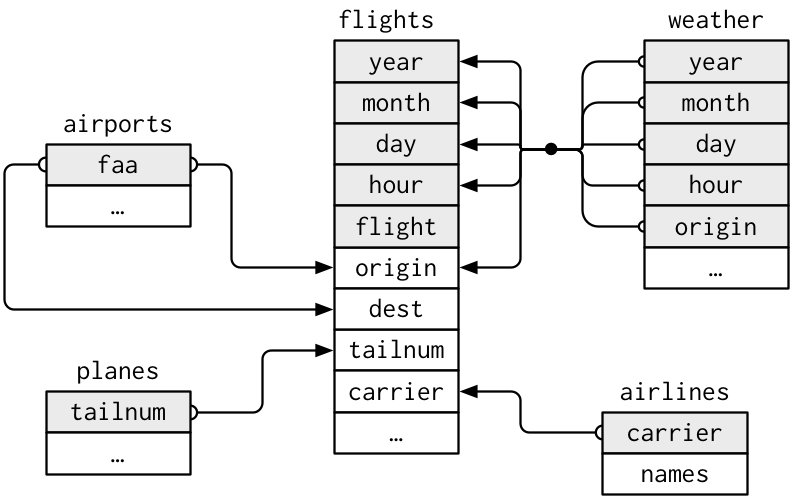
\includegraphics[width=\textwidth]{images/relational-nycflights} 

}

\caption[Data relationships in nycflights13 from R for Data Science]{Data relationships in nycflights13 from R for Data Science}\label{fig:reldiagram}
\end{figure}

We see from \texttt{View(airports)} that \texttt{airports} contains a
lot of other information about 1396. We are only really interested here
in the \texttt{faa} and \texttt{name} columns. Let's use the
\texttt{select} function to only use those variables:

\begin{Shaded}
\begin{Highlighting}[]
\NormalTok{airports_small <-}\StringTok{ }\NormalTok{airports %>%}
\StringTok{  }\KeywordTok{select}\NormalTok{(faa, name)}
\end{Highlighting}
\end{Shaded}

So if we identify the names of the airports we can use the
\texttt{inner\_join} function. Note that we will also rename the
subsequent column \texttt{name} as \texttt{airport\_name}:

\begin{Shaded}
\begin{Highlighting}[]
\NormalTok{named_freq_dests <-}\StringTok{ }\NormalTok{ten_freq_dests %>%}
\StringTok{  }\KeywordTok{inner_join}\NormalTok{(airports_small, }\DataTypeTok{by =} \KeywordTok{c}\NormalTok{(}\StringTok{"dest"} \NormalTok{=}\StringTok{ "faa"}\NormalTok{)) %>%}
\StringTok{  }\KeywordTok{rename}\NormalTok{(}\DataTypeTok{airport_name =} \NormalTok{name)}
\NormalTok{named_freq_dests}
\end{Highlighting}
\end{Shaded}

\begin{verbatim}
## # A tibble: 10 x 3
##     dest num_flights                       airport_name
##    <chr>       <int>                              <chr>
## 1    ORD       17283                 Chicago Ohare Intl
## 2    ATL       17215    Hartsfield Jackson Atlanta Intl
## 3    LAX       16174                   Los Angeles Intl
## 4    BOS       15508 General Edward Lawrence Logan Intl
## 5    MCO       14082                       Orlando Intl
## 6    CLT       14064             Charlotte Douglas Intl
## 7    SFO       13331                 San Francisco Intl
## 8    FLL       12055     Fort Lauderdale Hollywood Intl
## 9    MIA       11728                         Miami Intl
## 10   DCA        9705      Ronald Reagan Washington Natl
\end{verbatim}

In case you didn't know, \texttt{"ORD"} is the airport code of Chicago
O'Hare airport and \texttt{"FLL"} is the main airport in Fort
Lauderdale, Florida.

A visual representation of the \texttt{inner\_join} is given
\citep{rds2016}:

\begin{figure}

{\centering 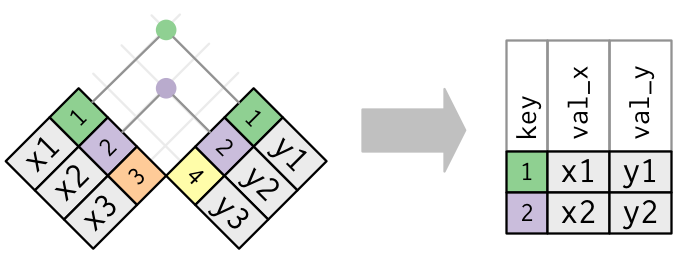
\includegraphics[width=\textwidth]{images/join-inner} 

}

\caption[Diagram of inner join from R for Data Science]{Diagram of inner join from R for Data Science}\label{fig:ijdiagram}
\end{figure}

There are more complex joins available, but the \texttt{inner\_join}
will solve nearly all (if not all) of the problems you'll face in our
experience.

\begin{center}\rule{0.5\linewidth}{\linethickness}\end{center}

\begin{learncheck}
\textbf{\emph{Learning check}}
\end{learncheck}

\textbf{(LC5.15)} What happens when you try to \texttt{inner\_join} the
\texttt{ten\_freq\_dests} data frame with \texttt{airports} instead of
\texttt{airports\_small}? How might one use this result to answer
further questions about the top 10 destinations?

\textbf{(LC5.16)} What surprises you about the top 10 destinations from
NYC in 2013?

\begin{center}\rule{0.5\linewidth}{\linethickness}\end{center}

\section{What's to come?}\label{whats-to-come-2}

This concludes the \textbf{Data Exploration} unit of this book. You
should be pretty proficient in both plotting variables (or multiple
variables together) in various data sets and manipulating data as we've
done in this chapter. You are encouraged to step back through the code
in earlier chapters and make changes as you see fit based on your
updated knowledge.

In Chapter \ref{infer-basics}, we'll begin to build the pieces needed to
understand how this unit of \textbf{Data Exploration} can tie into
statistical inference in the \textbf{Inference} part of the book.
Remember that the focus throughout is on data visualization and we'll
see that next when we discuss sampling, resampling, and bootstrapping.
These ideas will lead us into hypothesis testing and confidence
intervals.

\part{Inference}\label{part-inference}


\chapter{Inference Basics}\label{infer-basics}

In this chapter we will introduce new concepts that will serve as the
basis for the remainder of the text: \textbf{sampling},
\textbf{bootstrapping} and \textbf{resampling}. We will see that the
tools that you learned in the Data Exploration part of this book (tidy
data, data manipulation, and data visualization) will also play an
important role here. As mentioned before, the concepts all build into a
culmination allowing you to create better stories with data.

We begin with some helpful definitions that will help us better
understand why statistical inference exists and why it is needed. We
will then progress with a famous example from statistics lore and then
introduce the second of our main data sets (in addition to the
\texttt{nycflights13} data you've been working with) about movie ratings
from IMDB.com. We will see how we can use samples from this data set to
infer more general conclusions about all of the movies (in the
population).

\section{Random sampling}\label{random-sampling}

Whenever you hear the phrases ``random sampling'' or just ``sampling''
(with regards to statistics), you should think about tasting soup. This
likely sounds a little bonkers. Let's dig in to why tasting soup is such
an excellent analogy to random sampling.

\subsection{Tasting soup}\label{tasting-soup}

\begin{figure}

{\centering 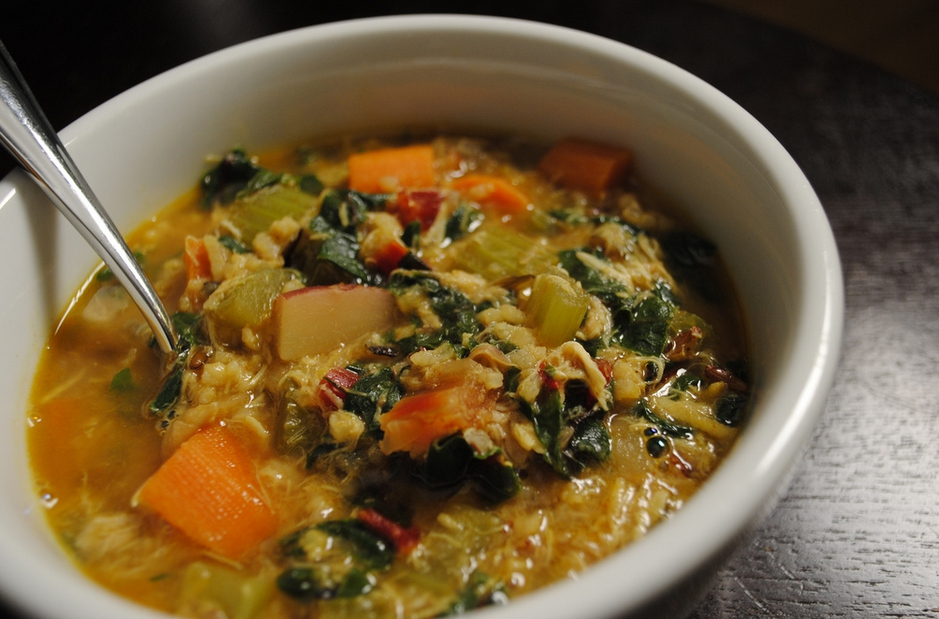
\includegraphics[width=\textwidth]{images/soup} 

}

\caption[A bowl of Indian chicken and vegetable soup]{A bowl of Indian chicken and vegetable soup}\label{fig:soupimg}
\end{figure}

Imagine that you have invited a group of friends over to try a new
recipe for soup that you've never made before. As in the image above
downloaded from
\href{http://readthespirit.wpengine.netdna-cdn.com/feed-the-spirit/wp-content/uploads/sites/19/2015/02/Chicken-soup-Indian-by-Fifth-Floor-Kitchen.jpg}{here},
you'd like to make a bowl of Indian chicken soup with lots of different
kinds of vegetables included.

You've carefully followed along with the recipe but you are concerned
that you don't have a lot of experience making Indian-style foods. It is
coming near the end of the prescribed time to cook given in the recipe.
You begin to wonder:

\begin{itemize}
\tightlist
\item
  ``Did I add too much curry spice?''
\item
  ``Are the carrots cooked enough?''\\
\item
  ``Does this actually taste good?''
\end{itemize}

How can we answer these questions? Does it matter where we take a bite
of soup from? Is there anything we should do to the soup before we
taste? Is one taste enough?

\begin{center}\rule{0.5\linewidth}{\linethickness}\end{center}

\begin{learncheck}
\textbf{\emph{Learning check}}
\end{learncheck}

\textbf{(LC6.1)} Explain in your own words how tasting soup relates to
the concepts of sampling covered here.

\textbf{(LC6.2)} Describe a different scenario (not food or drink
related) that is analogous to sampling concepts covered here.

\begin{center}\rule{0.5\linewidth}{\linethickness}\end{center}

\subsection{Common terms}\label{common-terms}

The process of sampling brings with it many common terms that we define
now. As you read over these definitions, think about how they each apply
to the tasting soup example above.

\begin{center}\rule{0.5\linewidth}{\linethickness}\end{center}

\textbf{Definition: population}

The \emph{population} is the (usually) large pool of observational units
that we are interested in.

\textbf{Definition: sample}

A \emph{sample} is a smaller collection of observational units that is
selected from the population.

\textbf{Definition: sampling}

\emph{Sampling} refers to the process of selecting observations from a
population. There are both random and non-random ways this can be done.

\textbf{Definition: representative sample}

A sample is said be a \emph{representative sample} if the
characteristics of observational units selected are a good approximation
of the characteristics from the original population.

\textbf{Definition: bias}

\emph{Bias} corresponds to a favoring of one group in a population over
another group.

\textbf{Definition: generalizability}

\emph{Generalizability} refers to the largest group in which it makes
sense to make inferences about from the sample collected. This is
directly related to how the sample was selected.

\textbf{Definition: parameter}

A \emph{parameter} is a calculation based on one or more variables
measured in the population. Parameters are almost always denoted
symbolically using Greek letters such as \(\mu\), \(\pi\), \(\sigma\),
\(\rho\), and \(\beta\).

\textbf{Definition: statistic}

A \emph{statistic} is a calculated based on one or more variables
measured in the sample. Parameters are usually denoted by lower case
Arabic letters with other symbols added sometimes. These include
\(\bar{x}\), \(\hat{p}\), \(s\), \(p\), and \(b\).

\begin{center}\rule{0.5\linewidth}{\linethickness}\end{center}

Let's explore these terms for our tasting soup example:

\emph{Population} - the entire container of soup that we have cooked.

\emph{Sample} - any smaller portion of soup collected that isn't the
whole container of soup. We could say that each spoonful of soup
represents one sample.

\emph{Sampling} - the process of selecting spoonfuls from the container
of soup

\emph{Representative sample} - A sample we select will only be
representative if it tastes like what the soup tastes like in general.
If we only select a carrot in our spoonful, we might not have a
representative sample.

\emph{Bias} - As we noted with the carrot selection example above, we
may select a sample that is not representative. If you watch chefs cook
or if you frequently cook, you'll be sure to stir the soup before you
taste it.

\emph{Generalizability} - If we stir our soup before we taste a spoonful
(and if we make sure we don't just pick our favorite item in the soup),
results from our sample can be generalized (by and large) to the larger
pot of soup. When we say ``Yum! This is good!'' after a couple
spoonfuls, we can be pretty confident that each bowl of soup for our
friends will taste good too.

\emph{Parameter} - An example here is could be the proportion of curry
entered into the entire pot of soup. A measurement of how salty the pot
of soup is on average is also a parameter. How crunchy, on average, the
carrots are in the pot of soup is one more example.

\emph{Statistic} - To convert a parameter to a statistic, you need only
to think about the same measurement on a spoonful:

\begin{itemize}
\tightlist
\item
  The proportion of curry to non-curry in a spoonful of soup
\item
  How salty the spoonful of soup is that we collected as our sample
\item
  How crunchy the carrots are in our spoonful of soup
\end{itemize}

\begin{center}\rule{0.5\linewidth}{\linethickness}\end{center}

\begin{learncheck}
\textbf{\emph{Learning check}}
\end{learncheck}

\textbf{(LC6.3)} Why isn't our population all bowls of soup? All bowls
of Indian chicken soup?

\textbf{(LC6.4)} Describe a way in which we could select a sample of
flights from \texttt{nycflights13} that is not representative.

\textbf{(LC6.5)} If we treat all of the flights in \texttt{nycflights13}
as the population, give examples of three \emph{parameters} we could
calculate.

\textbf{(LC6.6)} If we treat all of the flights in \texttt{nycflights13}
as the population, give examples of three \emph{statistics} we could
calculate.

\textbf{(LC6.7)} What biases might we see if we only select flights to
Boston when we are interested in looking at mean flight delays from NYC?

\begin{center}\rule{0.5\linewidth}{\linethickness}\end{center}

\section{Simulation}\label{simulation}

What follows is taken from a book entitled \emph{The Lady Tasting Tea}
\citep{salsburg2001}:

\begin{quote}
It was a summer afternoon in Cambridge, England, in the late 1920s. A
group of university dons, their wives, and some guests were sitting
around an outdoor table for afternoon tea. One of the women was
insisting that tea tasted different depending upon whether the tea was
poured into the milk or whether the milk was poured into the tea. The
scientific minds among the men scoffed at this as sheer nonsense. What
could be the difference? They could not conceive of any difference in
the chemistry of the mixtures that could exist. A thin, short man, with
thick glasses and a Vandyke beard beginning to turn gray, pounced on the
problem. ``Let us test the proposition,'' he said excitedly. He began to
outline an experiment in which the lady who insisted there was a
difference would be presented with a sequence of cups of tea, in some of
which the milk had been poured into the tea and in others of which the
tea had been poured into the milk\ldots{}
\end{quote}

\begin{quote}
So it was that sunny summer afternoon in Cambridge. The lady might or
might not have been correct about the tea infusion. The fun would be in
finding a way to determine if she was right, and, under the direction of
the man with the Vandyke beard, they began to discuss how they might
make that determination.
\end{quote}

\begin{quote}
Enthusiastically, many of them joined with him in setting up the
experiment. Within a few minutes, they were pouring different patterns
of infusion in a place where the lady could not see which cup was which.
Then, with an air of finality, the man with the Vandyke beard presented
her with her first cup. She sipped for a minute and declared that it was
one where the milk had been poured into the tea. He noted her response
without comment and presented her with the second cup\ldots{}
\end{quote}

\begin{quote}
The man with the Vandyke beard was Ronald Aylmer Fisher, who was in his
late thirties at the time. He would later be knighted Sir Ronald Fisher.
In 1935, he wrote a book entitled \emph{The Design of Experiments}, and
he described the experiment of the lady tasting tea in the second
chapter of that book. In his book, Fisher discusses the lady and her
belief as a hypothetical problem. He considers the various ways in which
an experiment might be designed to determine if she could tell the
difference. The problem in designing the experiment is that, if she is
given a single cup of tea, she has a 50 percent chance of guessing
correctly which infusion was used, even if she cannot tell the
difference. If she is given two cups of tea, she still might guess
correctly. In fact, if she knew that the two cups of tea were each made
with a different infusion, one guess could be completely right (or
completely wrong).
\end{quote}

\begin{quote}
Similarly, even if she could tell the difference, there is some chance
that she might have made a mistake, that one of the cups was not mixed
as well or that the infusion was made when the tea was not hot enough.
She might be presented with a series of ten cups and correctly identify
only nine of them, even if she could tell the difference.
\end{quote}

\begin{quote}
In his book, Fisher discusses the various possible outcomes of such an
experiment. He describes how to decide how many cups should be presented
and in what order and how much to tell the lady about the order of
presentations. He works out the probabilities of different outcomes,
depending upon whether the lady is or is not correct. Nowhere in this
discussion does he indicate that such an experiment was ever run. Nor
does he describe the outcome of an actual experiment.
\end{quote}

It's amazing that there is no actual evidence that such an event
actually took place. This problem is a great introduction into inference
though and we can proceed by testing to see how likely it is for a
person to guess correctly, say, 9 out of 10 times assuming that that
person is just guessing. In other words, is the person just lucky or do
we have reason to suspect that they can actually detect whether milk was
put in first or not?

We need to think about this problem from the standpoint of hypothesis
testing. First, we'll need to identify some important parts of a
hypothesis test before we proceed with the analysis.

\begin{center}\rule{0.5\linewidth}{\linethickness}\end{center}

\begin{learncheck}
\textbf{\emph{Learning check}}
\end{learncheck}

\textbf{(LC6.8)} What does ``by chance'' mean in this context?

\textbf{(LC6.9)} What is our observed statistic?

\textbf{(LC6.10)} What is this statistic trying to estimate?

\textbf{(LC6.11)} How could we test to see whether the person is just
guessing or if they have some special talent of identifying milk before
tea or vice-versa?

\begin{center}\rule{0.5\linewidth}{\linethickness}\end{center}

Let's begin with an experiment. I will flip a coin 10 times. Your job is
to try to predict the sequence of my 10 flips. Write down 10 H's and T's
corresponding to your predictions. We could compare your guesses with my
actual flips and then we will note how many correct guesses you have.

You may be asking yourself how this models a way to test whether the
person was just guessing or not. All we are trying to do is see how
likely it is to have 9 matches out of 10 if the person was truly
guessing. When we say ``truly guessing'' we are assuming that we have a
50/50 chance of guessing correctly. This can be modeled using a coin
flip and then seeing whether we guessed correctly for each of the coin
flips. If we guessed correctly, we can think of that as a ``success.''

We often don't have time to do the physical flipping over and over again
and we'd like to be able to do more than just 20 different simulations
or so. Luckily, we can use R to simulate this process many times. The
\texttt{mosaic} package includes a function called \texttt{rflip()},
which can be used to flip one coin. Well, not exactly. It uses
pseudo-random number generation to ``flip'' a virtual coin. In order for
us all to get the same results here, we can set the seed of the
pseudo-random number generator. Let's see an example of this: (Remember
to load the \texttt{mosaic} package!)

\begin{Shaded}
\begin{Highlighting}[]
\KeywordTok{library}\NormalTok{(mosaic)}
\KeywordTok{set.seed}\NormalTok{(}\DecValTok{2016}\NormalTok{)}
\KeywordTok{do}\NormalTok{(}\DecValTok{1}\NormalTok{) *}\StringTok{ }\KeywordTok{rflip}\NormalTok{(}\DecValTok{1}\NormalTok{)}
\end{Highlighting}
\end{Shaded}

\begin{verbatim}
##   n heads tails prop
## 1 1     0     1    0
\end{verbatim}

This shows us the proportion of ``successes'' in one flip of a coin. The
\texttt{do} function in the \texttt{mosaic} package will be useful and
you can begin to understand what it does with another example.

\begin{Shaded}
\begin{Highlighting}[]
\KeywordTok{do}\NormalTok{(}\DecValTok{13}\NormalTok{) *}\StringTok{ }\KeywordTok{rflip}\NormalTok{(}\DecValTok{10}\NormalTok{)}
\end{Highlighting}
\end{Shaded}

\begin{verbatim}
##     n heads tails prop
## 1  10     4     6  0.4
## 2  10     7     3  0.7
## 3  10     3     7  0.3
## 4  10     3     7  0.3
## 5  10     3     7  0.3
## 6  10     6     4  0.6
## 7  10     2     8  0.2
## 8  10     6     4  0.6
## 9  10     4     6  0.4
## 10 10     4     6  0.4
## 11 10     6     4  0.6
## 12 10     7     3  0.7
## 13 10     2     8  0.2
\end{verbatim}

We've now done a simulation of what actually happened when you flipped a
coin ten times. We have 13 different simulations of flipping a coin 10
times. Note here that \texttt{heads} now corresponds to the number of
correct guesses and \texttt{tails} corresponds to the number of
incorrect guesses. (This can be tricky to understand at first since
we've done a switch on what the meaning of ``heads'' and ``tails" are.)

If you look at the output above for our simulation of 13 student
guesses, we can begin to get a sense for what an ``expected'' sample
proportion of successes may be. Around five out of 10 seems to be the
most likely value. What does this say about our assumed \(\hat{p}\) of
9/10? To better answer this question, we can simulate 10,000 student
guesses and then look at the distribution of the simulated sample
proportion of successes, also known as the \textbf{null distribution}.

\begin{Shaded}
\begin{Highlighting}[]
\KeywordTok{library}\NormalTok{(dplyr)}
\KeywordTok{library}\NormalTok{(tibble)}
\NormalTok{simGuesses <-}\StringTok{ }\KeywordTok{do}\NormalTok{(}\DecValTok{10000}\NormalTok{) *}\StringTok{ }\KeywordTok{rflip}\NormalTok{(}\DecValTok{10}\NormalTok{)}
\NormalTok{simGuesses <-}\StringTok{ }\KeywordTok{as_tibble}\NormalTok{(simGuesses)}
\NormalTok{simGuesses %>%}\StringTok{ }
\StringTok{  }\KeywordTok{group_by}\NormalTok{(heads) %>%}
\StringTok{  }\KeywordTok{summarize}\NormalTok{(}\DataTypeTok{count =} \KeywordTok{n}\NormalTok{())}
\end{Highlighting}
\end{Shaded}

\begin{verbatim}
## # A tibble: 11 x 2
##    heads count
##    <dbl> <int>
## 1      0     7
## 2      1    81
## 3      2   424
## 4      3  1084
## 5      4  2075
## 6      5  2479
## 7      6  2117
## 8      7  1157
## 9      8   461
## 10     9   105
## 11    10    10
\end{verbatim}

\textbf{Note:} Here \texttt{as\_tibble} converts data frames to tibbles.
This is also why the \texttt{library(tibble)} command is needed. The
conversion to \texttt{tibble} format is mostly done for allowing for
nice printing of large data sets when we mention the name of a data
frame object in a chunk by itself. (The data sets in
\texttt{nycflights13} come as tibbles by default.) You can read more
about tibbles in Chapter 10 of Hadley and Garrett's book
\citep{rds2016}.

We can see here that we have created a count of how many of each of the
10,000 sets of 10 flips resulted in 0, 1, 2, \ldots{}, up to 10 heads.
Note the use of the \texttt{group\_by} and \texttt{summarize} functions
from Chapter \ref{manip} here.

In addition, we can plot the distribution of these simulated
\texttt{heads} using the ideas from Chapter \ref{viz}. \texttt{heads} is
a quantitative variable. Think about which type of plot is most
appropriate here before reading further.

We already have an idea as to an appropriate plot by the data
summarization that we did in the chunk above. We'd like to see how many
heads occurred in the 10,000 sets of 10 flips. In other words, we'd like
to see how frequently 9 or more heads occurred in the 10 flips:

\begin{Shaded}
\begin{Highlighting}[]
\KeywordTok{library}\NormalTok{(ggplot2)}
\NormalTok{simGuesses %>%}\StringTok{ }\KeywordTok{ggplot}\NormalTok{(}\KeywordTok{aes}\NormalTok{(}\DataTypeTok{x =} \NormalTok{heads)) +}
\StringTok{  }\KeywordTok{geom_bar}\NormalTok{()}
\end{Highlighting}
\end{Shaded}

\begin{figure}

{\centering 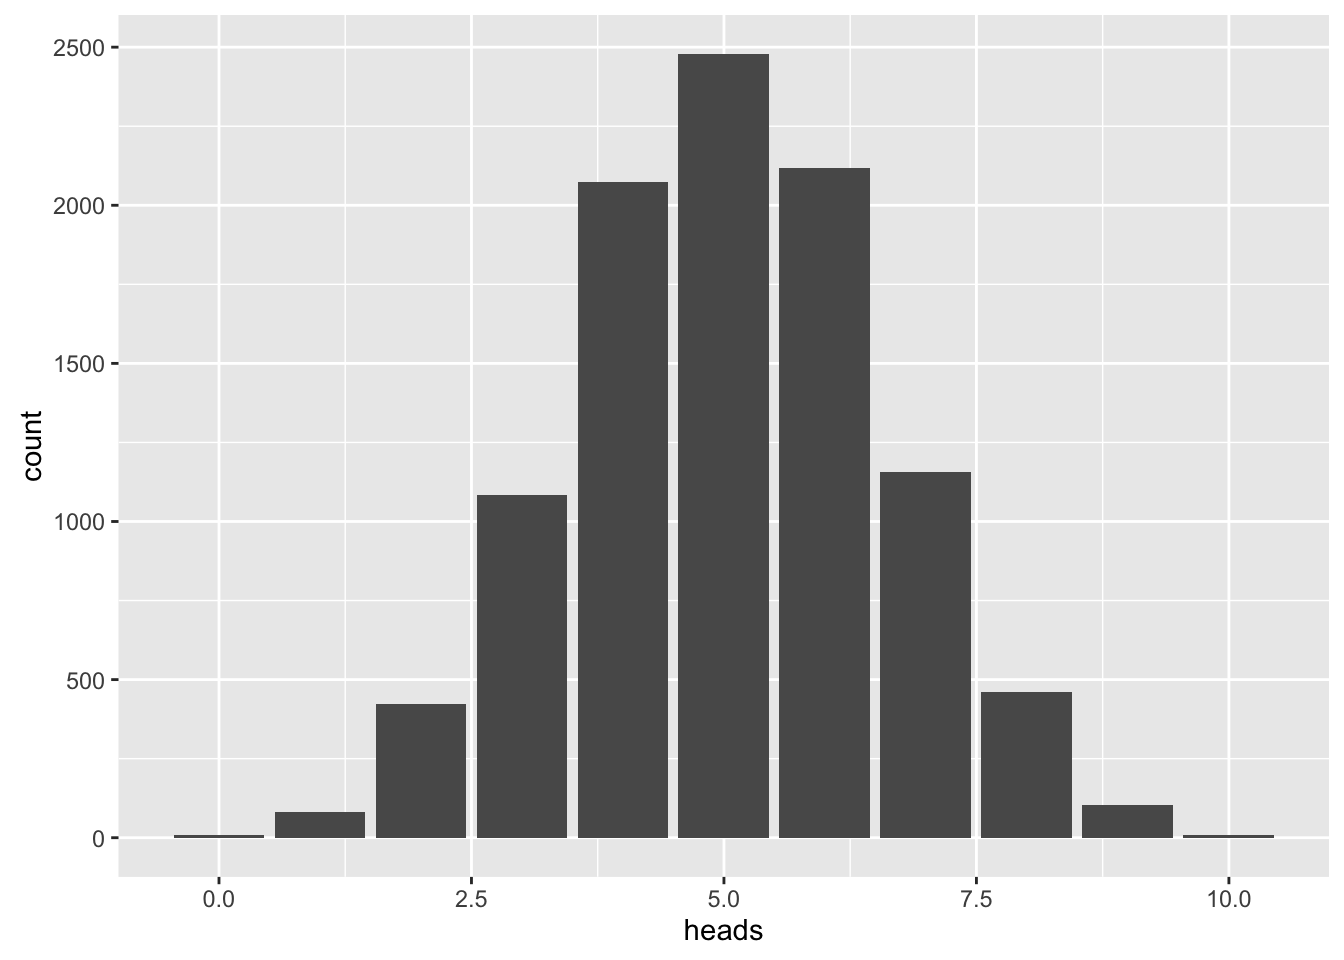
\includegraphics[width=\textwidth]{ismay_files/figure-latex/unnamed-chunk-75-1} 

}

\caption[Barplot of number of heads in simulation - needs tweaking]{Barplot of number of heads in simulation - needs tweaking}\label{fig:unnamed-chunk-75}
\end{figure}

This horizontal axis labels are a little confusing here. What does 2.5
or 7.5 heads mean? In \texttt{simGuesses}, \texttt{heads} is a
\texttt{numerical} variable. Thus, \texttt{ggplot} is expecting the
values to be on a continuous scale. We can switch the scale to be
discrete by invoking the \texttt{factor} function:

\begin{Shaded}
\begin{Highlighting}[]
\KeywordTok{library}\NormalTok{(ggplot2)}
\NormalTok{simGuesses %>%}\StringTok{ }\KeywordTok{ggplot}\NormalTok{(}\KeywordTok{aes}\NormalTok{(}\DataTypeTok{x =} \KeywordTok{factor}\NormalTok{(heads))) +}
\StringTok{  }\KeywordTok{geom_bar}\NormalTok{()}
\end{Highlighting}
\end{Shaded}

\begin{figure}

{\centering 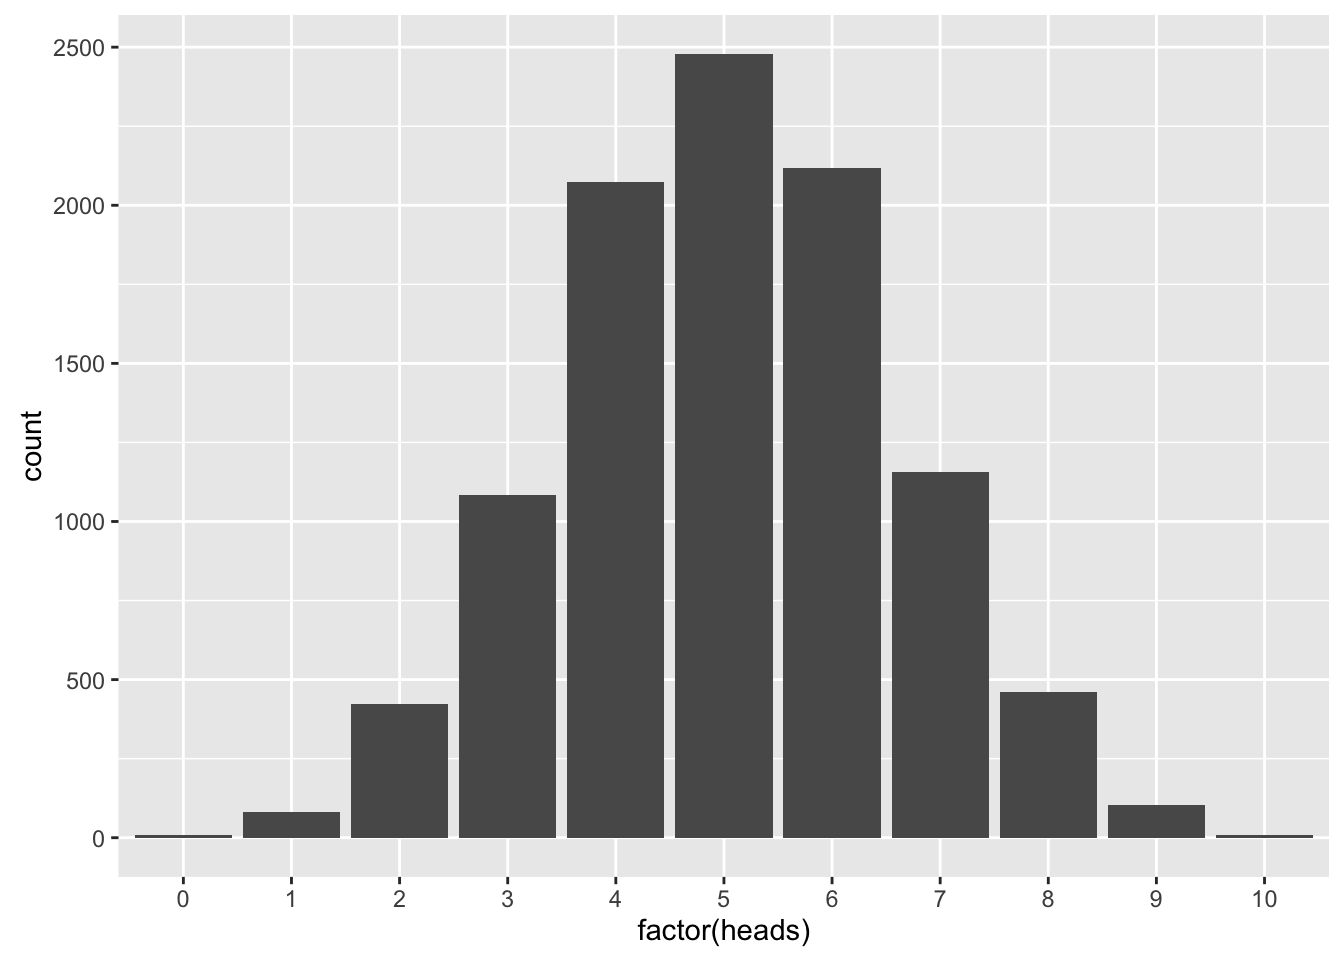
\includegraphics[width=\textwidth]{ismay_files/figure-latex/unnamed-chunk-76-1} 

}

\caption[Barplot of number of heads in simulation]{Barplot of number of heads in simulation}\label{fig:unnamed-chunk-76}
\end{figure}

You'll frequently need to make this conversion to \texttt{factor} when
making a barplot with quantitative variables. Remember from ``Getting
Used to R, RStudio, and R Markdown'' \citep{usedtor2016}, that a
\texttt{factor} variable is useful when there is a natural ordering to
the variable. Our \texttt{heads} variable has a natural ordering: 0, 1,
2, \ldots{}, 10.

\subsection{The p-value}\label{the-p-value}

\begin{center}\rule{0.5\linewidth}{\linethickness}\end{center}

\textbf{Definition: \(p\)-value}:

The \textbf{p-value} is the probability of observing a sample statistic
as extreme or more extreme than what was observed, assuming that the
null hypothesis of a by chance operation is true.

\begin{center}\rule{0.5\linewidth}{\linethickness}\end{center}

This definition may be a little intimidating the first time you read it,
but it's important to come back to this ``The Lady Tasting Tea'' problem
whenever you encounter \(p\)-values as you begin to learn about the
concept. Here the \(p\)-value corresponds to how many times in our
\textbf{null distribution} of \texttt{heads} 9 or more heads occurred.

We can use another neat feature of R to calculate the \(p\)-value for
this problem. Note that ``more extreme'' in this case corresponds to
looking at values of 9 or greater since our alternative hypothesis
invokes a right-tail test corresponding to a ``greater than'' hypothesis
of \(H_a: \pi > 0.5\). In other words, we are looking to see how likely
it is for the lady to pick 9 or more correct instead of 9 or less
correct. We'd like to go in the right direction.

\begin{Shaded}
\begin{Highlighting}[]
\NormalTok{pvalue_tea <-}\StringTok{ }\NormalTok{simGuesses %>%}
\StringTok{  }\KeywordTok{filter}\NormalTok{(heads >=}\StringTok{ }\DecValTok{9}\NormalTok{) %>%}
\StringTok{  }\KeywordTok{nrow}\NormalTok{() /}\StringTok{ }\KeywordTok{nrow}\NormalTok{(simGuesses)}
\end{Highlighting}
\end{Shaded}

Let's walk through each step of this calculation:

\begin{enumerate}
\def\labelenumi{\arabic{enumi}.}
\item
  First, \texttt{pvalue\_tea} will be the name of our calculated
  \(p\)-value and the assignment operator \texttt{\textless{}-} directs
  us to this naming.
\item
  We are working with the \texttt{simGuesses} data frame here so that
  comes immediately before the pipe operator.
\item
  We would like to only focus on the rows in our \texttt{simGuesses}
  data frame that have \texttt{heads} values of 9 or 10. This represents
  simulated statistics ``as extreme or more extreme'' than what we
  observed (9 correct guesses out of 10). Let's get a glimpse of what we
  have up to this point:

\begin{Shaded}
\begin{Highlighting}[]
\NormalTok{simGuesses %>%}\StringTok{ }\KeywordTok{tbl_df}\NormalTok{() %>%}
\StringTok{  }\KeywordTok{filter}\NormalTok{(heads >=}\StringTok{ }\DecValTok{9}\NormalTok{)    }
\end{Highlighting}
\end{Shaded}

\begin{verbatim}
## # A tibble: 115 x 4
##        n heads tails  prop
##    <dbl> <dbl> <dbl> <dbl>
## 1     10     9     1   0.9
## 2     10     9     1   0.9
## 3     10     9     1   0.9
## 4     10     9     1   0.9
## 5     10     9     1   0.9
## 6     10     9     1   0.9
## 7     10    10     0   1.0
## 8     10     9     1   0.9
## 9     10     9     1   0.9
## 10    10     9     1   0.9
## # ... with 105 more rows
\end{verbatim}
\item
  Now that we have changed the focus to only those rows that have number
  of heads out of 10 flips corresponding to 9 or more, we count how many
  of those there are. The function \texttt{nrow} gives how many entries
  are in this filtered data frame and lastly we calculate the proportion
  that are at least as extreme as our observed value of 9 by dividing by
  the number of total simulations (10,000).
\end{enumerate}

We can see that the observed statistic of 9 correct guesses is not a
likely outcome assuming the null hypothesis is true. Only around 1\% of
the outcomes in our 10,000 simulations fall at or above 9 successes. We
have evidence supporting the conclusion that the person is actually
better than just guessing at random at determining whether milk has been
added first or not. To better visualize this we can also make use of
pink shading on the histogram corresponding to the \(p\)-value:

\begin{Shaded}
\begin{Highlighting}[]
\KeywordTok{library}\NormalTok{(ggplot2)}
\NormalTok{simGuesses %>%}\StringTok{ }
\StringTok{  }\KeywordTok{ggplot}\NormalTok{(}\KeywordTok{aes}\NormalTok{(}\DataTypeTok{x =} \KeywordTok{factor}\NormalTok{(heads), }\DataTypeTok{fill =} \NormalTok{(heads >=}\StringTok{ }\DecValTok{9}\NormalTok{))) +}
\StringTok{  }\KeywordTok{geom_bar}\NormalTok{() +}
\StringTok{  }\KeywordTok{labs}\NormalTok{(}\DataTypeTok{x =} \StringTok{"heads"}\NormalTok{)}
\end{Highlighting}
\end{Shaded}

\begin{figure}

{\centering 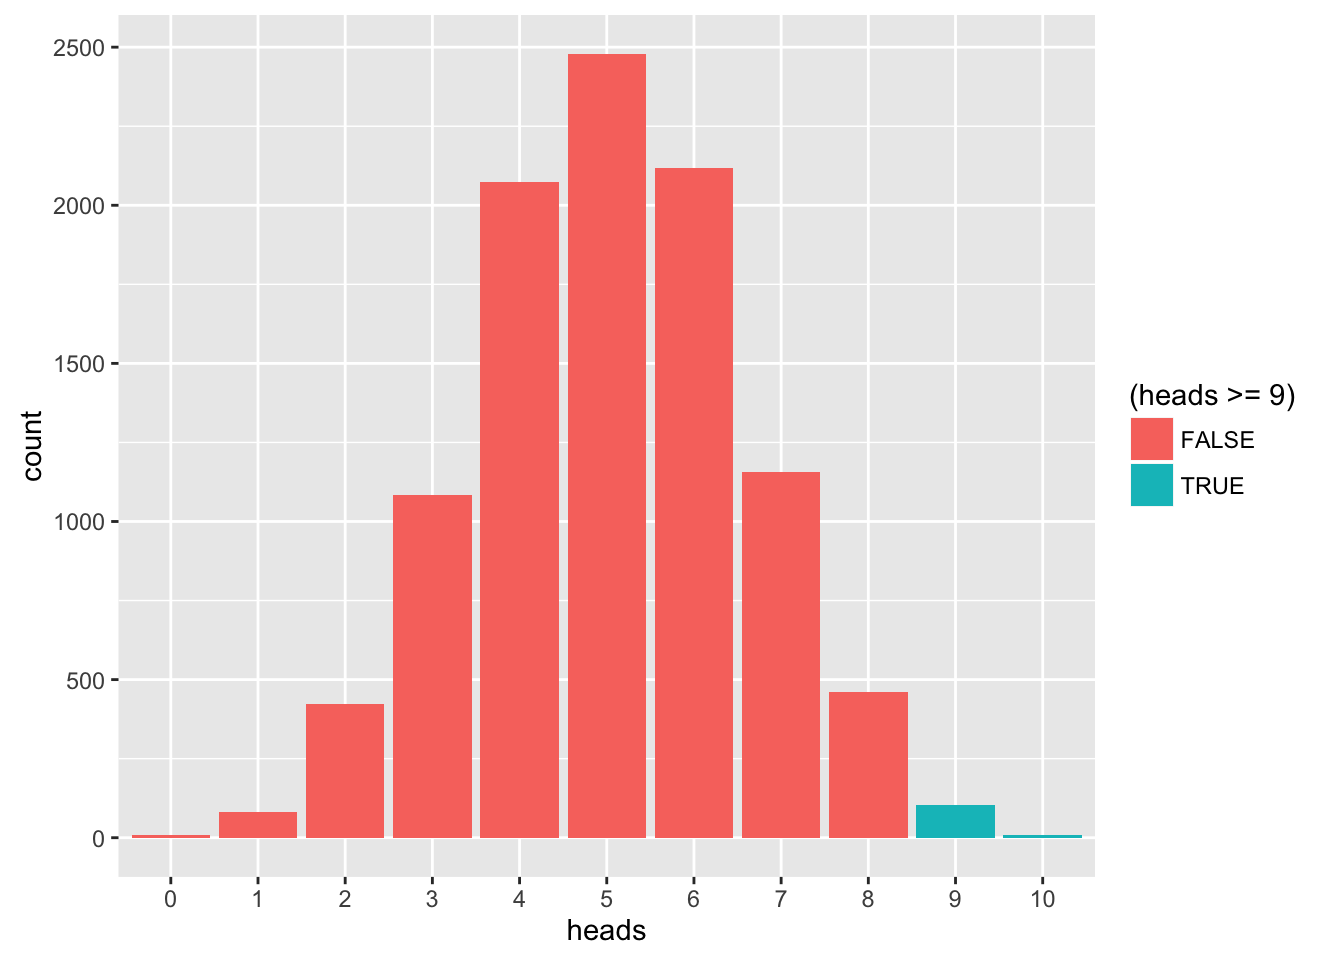
\includegraphics[width=\textwidth]{ismay_files/figure-latex/unnamed-chunk-79-1} 

}

\caption[Barplot of heads with p-value highlighted]{Barplot of heads with p-value highlighted}\label{fig:unnamed-chunk-79}
\end{figure}

This helps us better see just how few of the values of \texttt{heads}
are at our observed value or more extreme.

We'll see in Chapters \ref{hypo} and \ref{ci} that this idea of a
\(p\)-value can be extended to the more traditional methods using normal
and \(t\) distributions in the traditional way that introductory
statistics has been presented. These traditional methods were used
because statisticians haven't always been able to do 10,000 simulations
on the computer within seconds. We'll elaborate on this more in these
later chapters.

\begin{center}\rule{0.5\linewidth}{\linethickness}\end{center}

\begin{learncheck}
\textbf{\emph{Learning check}}
\end{learncheck}

\textbf{(LC6.12)} What is meant by ``pseudo-random number generation?''

\textbf{(LC6.13)} How can simulation be used to help us address the
question of whether or not an observed result is statistically
significant?

\textbf{(LC6.14)} In Chapter \ref{viz}, we noted that barplots should be
used when creating a plot of categorical variables. Why are we using
barplots to make a plot of a numerical variable \texttt{heads} in this
chapter?

\begin{center}\rule{0.5\linewidth}{\linethickness}\end{center}

\section{Bootstrapping}\label{bootstrapping}

Just as we did in the previous section when making hypotheses about a
population proportion with which we would like to test which one is more
plausible, we can also use simulation to infer conclusions about a
population quantitative statistic such as the mean. In this case, we
will focus on constructing confidence intervals to produce plausible
values for a population mean. (We can do a similar analysis for a
population median or other summary measure as well.)

Traditionally, the way to construct confidence intervals for a mean is
to assume a normal distribution for the population or to invoke the
Central Limit Theorem and get, what often appears to be magic, results.
These methods are often not intuitive, especially for those that lack a
strong mathematical background. They also come with their fair share of
assumptions and often turn Statistics, a field that is full of tons of
useful applications to many different fields and disciplines, into a
robotic procedural-based topic. It doesn't have to be that way!

In this section, we will introduce the concept of
\textbf{bootstrapping}. It will be a useful tool that will allow us to
estimate the variability of our statistic from sample to sample. One
neat feature of bootstrapping is that it enables us to approximate the
sampling distribution and estimate the distribution's standard deviation
using ONLY the information in the one selected (original) sample.

It sounds just as plagued with the magical type qualities of traditional
theory-based inference on initial glance but we will see that it
provides an intuitive and useful way to make inferences, especially when
the samples are of medium to large size.

To introduce the concept of bootstrapping, we now introduce the
\texttt{movies} data set in the \texttt{ggplot2movies} data frame. We
will load this data frame into R in much the same way as we loaded
\texttt{flights} and \texttt{weather} from the \texttt{nycflights13}
package:

\begin{Shaded}
\begin{Highlighting}[]
\KeywordTok{library}\NormalTok{(ggplot2movies)}
\KeywordTok{data}\NormalTok{(movies, }\DataTypeTok{package =} \StringTok{"ggplot2movies"}\NormalTok{)}
\end{Highlighting}
\end{Shaded}

Let's also glance at this data frame using the \texttt{View} function
and look at the help documentation for \texttt{movies}:

\begin{Shaded}
\begin{Highlighting}[]
\KeywordTok{View}\NormalTok{(movies)}
\NormalTok{?movies}
\end{Highlighting}
\end{Shaded}

We will explore many other features of this data set in the chapters to
come, but here we will be focusing on the \texttt{rating} variable
corresponding to the average IMDB user rating.

You may notice that this data set is quite large: 58,788 movies have
data collected about them here. This will correspond to our population
of ALL movies. Remember from Chapter \ref{infer-basics} that our
population is rarely known. We use this data set as our population here
to show you the power of bootstrapping in estimating population
parameters. We'll see how \textbf{confidence intervals} built using the
bootstrap distribution do at including our population parameter of
interest. Here we can actually calculate these values since our
population is known, but remember that in general this isn't the case.

Let's take a look at what the distribution of our population
\texttt{ratings} looks like. We'll see that we will use the distribution
of our sample(s) as an estimate of this population histogram.

\begin{Shaded}
\begin{Highlighting}[]
\NormalTok{movies %>%}\StringTok{ }\KeywordTok{ggplot}\NormalTok{(}\KeywordTok{aes}\NormalTok{(}\DataTypeTok{x =} \NormalTok{rating)) +}
\StringTok{  }\KeywordTok{geom_histogram}\NormalTok{(}\DataTypeTok{color =} \StringTok{"white"}\NormalTok{, }\DataTypeTok{bins =} \DecValTok{20}\NormalTok{)}
\end{Highlighting}
\end{Shaded}

\begin{figure}

{\centering 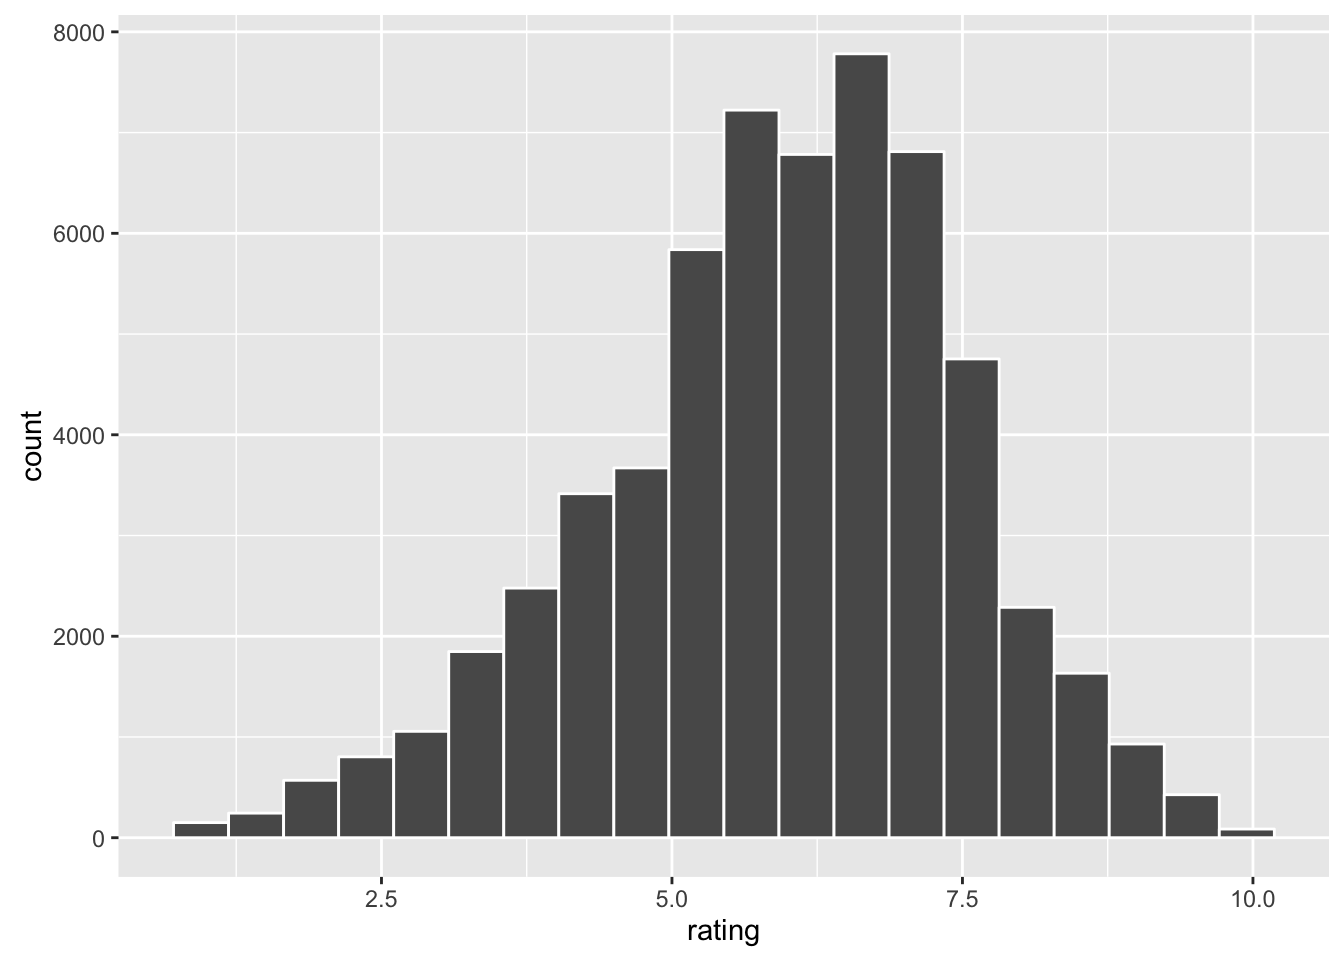
\includegraphics[width=\textwidth]{ismay_files/figure-latex/unnamed-chunk-82-1} 

}

\caption[Population ratings histogram]{Population ratings histogram}\label{fig:unnamed-chunk-82}
\end{figure}

\begin{center}\rule{0.5\linewidth}{\linethickness}\end{center}

\begin{learncheck}
\textbf{\emph{Learning check}}
\end{learncheck}

\textbf{(LC6.15)} Why was a histogram chosen as the plot to make for the
\texttt{rating} variable above?

\textbf{(LC6.16)} Why does the shape of the \texttt{rating} histogram
tell us about how IMDB users rate movies? What stands out about the
plot?

\begin{center}\rule{0.5\linewidth}{\linethickness}\end{center}

It's important to think about what our goal is here. We would like to
produce a confidence interval for the population mean \texttt{rating}.
We will have to pretend for a moment that we don't have all 58,788
movies. Let's say that we only have a random sample of 50 movies from
this data set instead. In order to get a random sample, we can use the
\texttt{sample\_n} function from \texttt{dplyr}:

\begin{Shaded}
\begin{Highlighting}[]
\KeywordTok{set.seed}\NormalTok{(}\DecValTok{2016}\NormalTok{)}
\NormalTok{movies_sample <-}\StringTok{ }\NormalTok{movies %>%}
\StringTok{  }\KeywordTok{sample_n}\NormalTok{(}\DecValTok{50}\NormalTok{)}
\end{Highlighting}
\end{Shaded}

The \texttt{sample\_n} function has filtered the data frame
\texttt{movies} ``at random'' to choose only 50 rows from the larger
\texttt{movies} data frame. We store information on these 50 movies in
the \texttt{movies\_sample} data frame.

Let's now explore what the \texttt{rating} variable looks like for these
50 movies:

\begin{Shaded}
\begin{Highlighting}[]
\NormalTok{movies_sample %>%}\StringTok{ }\KeywordTok{ggplot}\NormalTok{(}\KeywordTok{aes}\NormalTok{(}\DataTypeTok{x =} \NormalTok{rating)) +}
\StringTok{  }\KeywordTok{geom_histogram}\NormalTok{(}\DataTypeTok{color =} \StringTok{"white"}\NormalTok{, }\DataTypeTok{bins =} \DecValTok{20}\NormalTok{)}
\end{Highlighting}
\end{Shaded}

\begin{figure}

{\centering 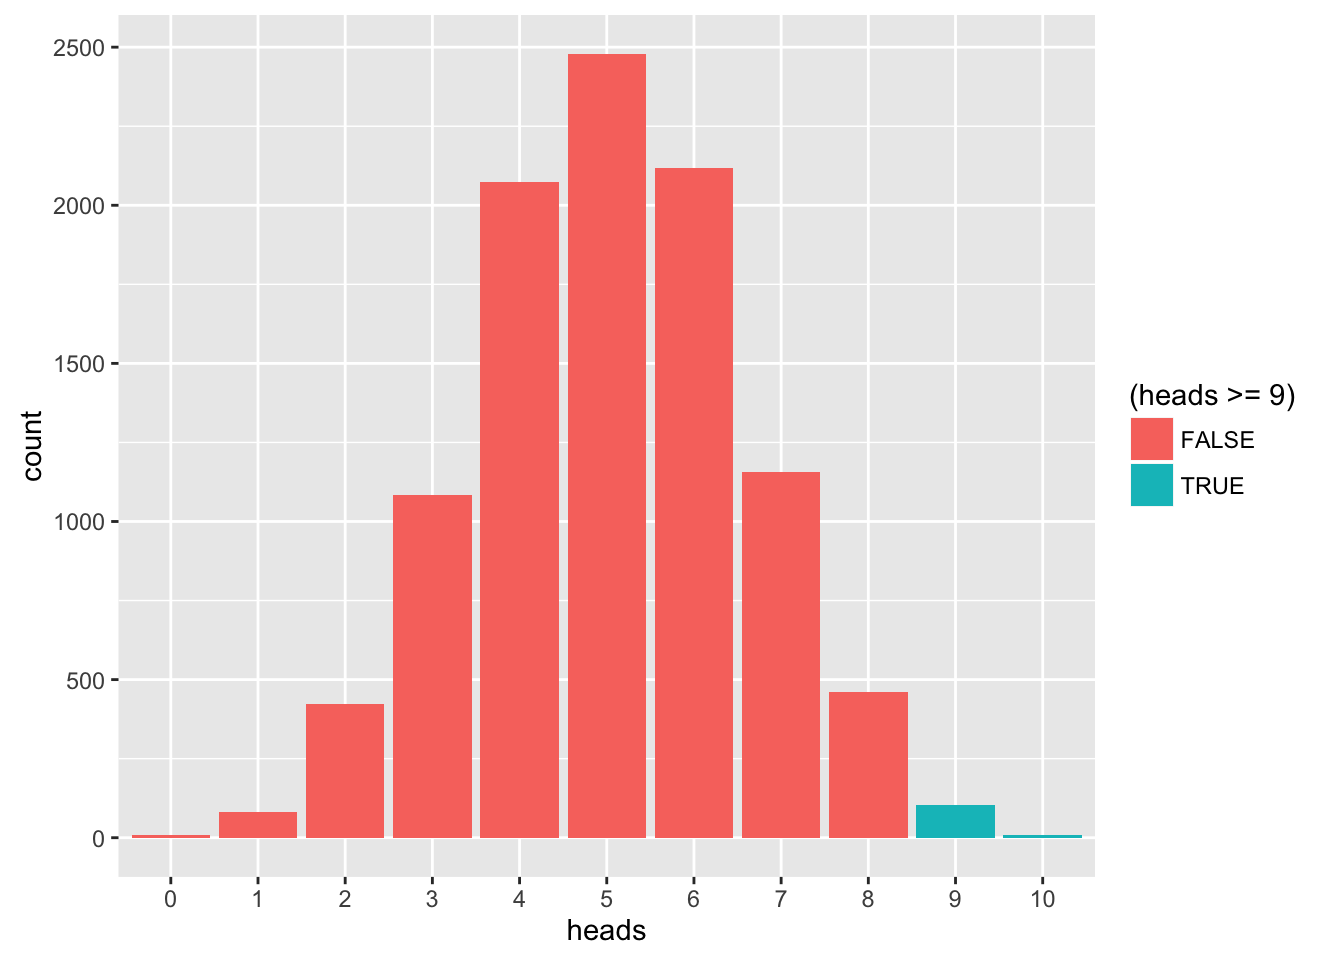
\includegraphics[width=\textwidth]{ismay_files/figure-latex/unnamed-chunk-84-1} 

}

\caption[Sample ratings histogram]{Sample ratings histogram}\label{fig:unnamed-chunk-84}
\end{figure}

Remember that we can think of this histogram as an estimate of our
population distribution histogram that we saw above. We are interested
in the population mean rating and trying to find a range of plausible
values for that value. A good start in guessing the population mean is
to use the mean of our sample \texttt{rating} from the
\texttt{movies\_sample} data:

\begin{Shaded}
\begin{Highlighting}[]
\NormalTok{(movies_sample_mean <-}\StringTok{ }\NormalTok{movies_sample %>%}\StringTok{ }\KeywordTok{summarize}\NormalTok{(}\DataTypeTok{mean =} \KeywordTok{mean}\NormalTok{(rating)))}
\end{Highlighting}
\end{Shaded}

\begin{verbatim}
## # A tibble: 1 x 1
##    mean
##   <dbl>
## 1 6.034
\end{verbatim}

Note the use of the \texttt{(\ )} at the beginning and the end of this
creation of the \texttt{movies\_sample\_mean} object. If you'd like to
print out your newly created object, you can enclose it in the
parentheses as we have here.

This value of 6.034 is just one guess at the population mean. The idea
behind \emph{bootstrapping} is to sample \textbf{with replacement} from
the original sample to create new \textbf{resamples} of the same size as
our original sample.

Returning to our example, let's investigate what one such resample of
the \texttt{movies\_sample} data set accomplishes. We can create one
resample/bootstrap sample by using the \texttt{resample} function in the
\texttt{mosaic} package.

\begin{Shaded}
\begin{Highlighting}[]
\KeywordTok{library}\NormalTok{(mosaic)}
\KeywordTok{library}\NormalTok{(tibble)}
\NormalTok{boot1 <-}\StringTok{ }\KeywordTok{resample}\NormalTok{(movies_sample, }\DataTypeTok{orig.ids =} \OtherTok{TRUE}\NormalTok{) %>%}
\StringTok{  }\KeywordTok{select}\NormalTok{(orig.id, }\KeywordTok{everything}\NormalTok{()) %>%}
\StringTok{  }\KeywordTok{arrange}\NormalTok{(orig.id)}
\end{Highlighting}
\end{Shaded}

Take a look at this resample/bootstrap:

\begin{Shaded}
\begin{Highlighting}[]
\KeywordTok{View}\NormalTok{(boot1)}
\end{Highlighting}
\end{Shaded}

The important thing to note here is the original row numbers from the
\texttt{movies\_sample} data frame in the far left column called
\texttt{orig.ids}. Since we are sampling with replacement, there is a
strong likelihood that some of the 50 observational units are going to
be selected again.

You may be asking yourself what does this mean and how to this lead us
to creating a distribution for the sample mean. Recall that the original
sample mean of our data was calculated using the \texttt{summarize}
function above.

\begin{center}\rule{0.5\linewidth}{\linethickness}\end{center}

\begin{learncheck}
\textbf{\emph{Learning check}}
\end{learncheck}

\textbf{(LC6.17)} What happens if we change the seed to our
pseudo-random generation? Try it above when we used \texttt{sample\_n}
to describe the resulting \texttt{movies\_sample}.

\textbf{(LC6.18)} Why is sampling at random important from the
\texttt{movies} data frame? Why don't we just pick \texttt{Action}
movies and do bootstrapping with this \texttt{Action} movies subset?

\textbf{(LC6.19)} What was the purpose of assuming we didn't have access
to the full \texttt{movies} data set here?

\begin{center}\rule{0.5\linewidth}{\linethickness}\end{center}

Before we had a calculated mean in our original sample of 6.034. Let's
calculate the mean of \texttt{ratings} in our bootstrapped sample:

\begin{Shaded}
\begin{Highlighting}[]
\NormalTok{(movies_boot1_mean <-}\StringTok{ }\NormalTok{boot1 %>%}\StringTok{ }\KeywordTok{summarize}\NormalTok{(}\DataTypeTok{mean =} \KeywordTok{mean}\NormalTok{(rating)))}
\end{Highlighting}
\end{Shaded}

\begin{verbatim}
## # A tibble: 1 x 1
##    mean
##   <dbl>
## 1 6.144
\end{verbatim}

More than likely the calculated bootstrap sample mean is different than
the original sample mean. This is what I meant earlier when I said that
the sample means have some variability. What we are trying to do is
replicate many different samples being taken from a larger population.
Our best guess at what the population looks like is multiple copies of
the sample we collected. We then can sample from that larger ``created''
population by generating bootstrap samples.

Similar to what we did in the previous section, we can repeat this
process using the \texttt{do} function followed by an asterisk. Let's
look at 10 different bootstrap means for \texttt{ratings} from
\texttt{movies\_sample}. Note the use of the \texttt{resample} function
here.

\begin{Shaded}
\begin{Highlighting}[]
\KeywordTok{do}\NormalTok{(}\DecValTok{10}\NormalTok{) *}\StringTok{ }\KeywordTok{summarize}\NormalTok{(}\KeywordTok{resample}\NormalTok{(movies_sample), }\DataTypeTok{mean =} \KeywordTok{mean}\NormalTok{(rating))}
\end{Highlighting}
\end{Shaded}

\begin{verbatim}
##     mean
## 1  6.020
## 2  6.668
## 3  5.996
## 4  6.056
## 5  6.168
## 6  6.360
## 7  5.702
## 8  6.218
## 9  6.252
## 10 5.904
\end{verbatim}

You should see some variability begin to tease its way out here. Many of
the simulated means will be close to our original sample mean but many
will stray pretty far away. This occurs because outliers may have been
selected a couple of times in the resampling or small values were
selected more than larger. There are myriad reasons why this might be
the case.

So what's the next step now? Just as we repeated the repetitions
thousands of times with the ``Lady Tasting Tea'' example, we can do a
similar thing here.

\begin{Shaded}
\begin{Highlighting}[]
\NormalTok{trials <-}\StringTok{ }\KeywordTok{do}\NormalTok{(}\DecValTok{10000}\NormalTok{) *}\StringTok{ }\KeywordTok{summarize}\NormalTok{(}\KeywordTok{resample}\NormalTok{(movies_sample), }
                                \DataTypeTok{mean =} \KeywordTok{mean}\NormalTok{(rating))}
\NormalTok{trials %>%}\StringTok{ }\KeywordTok{ggplot}\NormalTok{(}\KeywordTok{aes}\NormalTok{(}\DataTypeTok{x =} \NormalTok{mean)) +}
\StringTok{  }\KeywordTok{geom_histogram}\NormalTok{(}\DataTypeTok{bins =} \DecValTok{30}\NormalTok{, }\DataTypeTok{color =} \StringTok{"white"}\NormalTok{)}
\end{Highlighting}
\end{Shaded}

\begin{figure}

{\centering 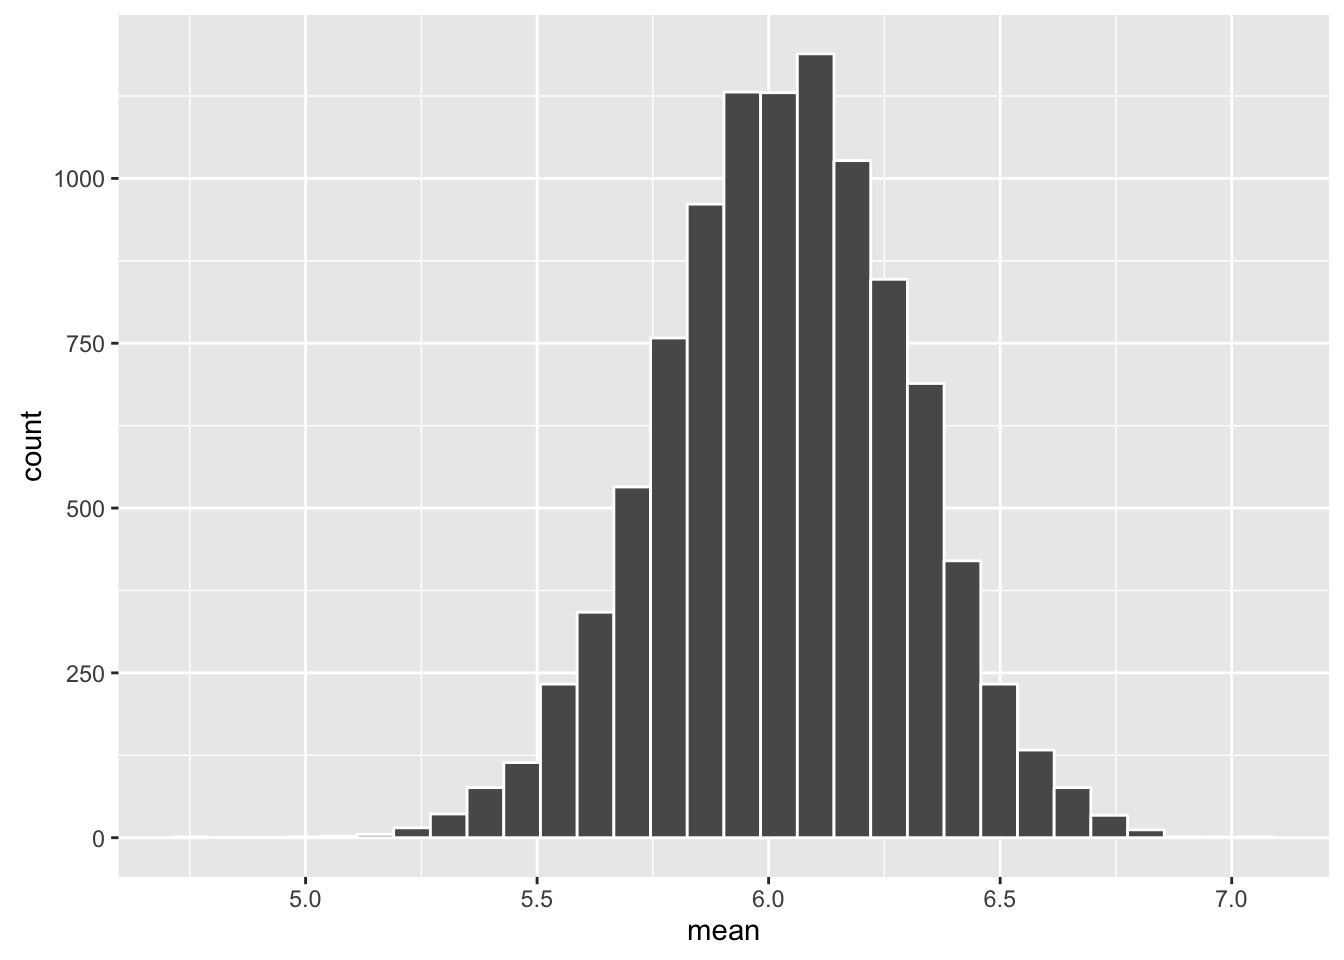
\includegraphics[width=\textwidth]{ismay_files/figure-latex/unnamed-chunk-90-1} 

}

\caption[Bootstrapped means histogram]{Bootstrapped means histogram}\label{fig:unnamed-chunk-90}
\end{figure}

The shape of this resulting distribution may look familiar to you. It
resembles the well-known normal (bell-shaped) curve. We will see in
Chapters \ref{hypo} and \ref{ci} when we might expect a normal curve to
come through as we have here and when we shouldn't. There will be
specific assumptions that need to be checked and we will see that the
normal distribution doesn't always approximate this bootstrapped
distribution well. In those case, we should NOT rely on traditional
methods.

At this point, we can easily calculate a confidence interval. In fact,
we have a couple different options. We will first use the percentiles of
the distribution we just created to isolate the middle 95\% of values.
This will correspond to our 95\% confidence interval for the population
mean \texttt{rating}, denoted by \(\mu\).

\begin{Shaded}
\begin{Highlighting}[]
\NormalTok{(ciq_mean_rating <-}\StringTok{ }\KeywordTok{confint}\NormalTok{(trials, }\DataTypeTok{level =} \FloatTok{0.95}\NormalTok{, }\DataTypeTok{method =} \StringTok{"quantile"}\NormalTok{))}
\end{Highlighting}
\end{Shaded}

\begin{verbatim}
##   name   lower upper level     method estimate
## 1 mean 5.50795  6.54  0.95 percentile    6.034
\end{verbatim}

It's always important at this point to interpret the results of this
confidence interval calculation. In this context, we can say something
like the following:

\begin{quote}
Based on the sample data and bootstrapping techniques, we can be 95\%
confident that the true mean rating of ALL IMDB ratings is between
5.50795 and 6.54.
\end{quote}

This statement may seem a little confusing to you. Remember that we are
pretending like we don't know what the mean IMDB rating for ALL movies
is. Our population here is all of the movies listed in the
\texttt{movies} data frame from \texttt{ggplot2movies}. So does our
bootstrapped confidence interval here contain the actual mean value?

\begin{Shaded}
\begin{Highlighting}[]
\KeywordTok{summarize}\NormalTok{(movies, }\DataTypeTok{mean =} \KeywordTok{mean}\NormalTok{(rating))}
\end{Highlighting}
\end{Shaded}

\begin{verbatim}
## # A tibble: 1 x 1
##      mean
##     <dbl>
## 1 5.93285
\end{verbatim}

We see here that the population mean does fall in our range of plausible
values generated from the bootstrapped samples.

We can also get an idea of how the theory-based inference techniques
would have approximated this confidence interval by using the formula
\[\bar{x} \pm (2 * SE),\] where \(\bar{x}\) is our original sample mean
and \(SE\) stands for \textbf{standard error} and corresponds to the
standard deviation of the bootstrap distribution. The value of 2 here
corresponds to it being a 95\% confidence interval. This formula assumes
that the bootstrap distribution is symmetric. This is often the case
with bootstrap distributions, especially those in which the original
distribution of the sample is not highly skewed.

To compute this type of confidence interval, we only need to make a
slight modification to the \texttt{confint} function seen above. (The
expression after the \(\pm\) sign is known as the \textbf{margin of
error}.)

\begin{Shaded}
\begin{Highlighting}[]
\NormalTok{(cise_mean_rating <-}\StringTok{ }\KeywordTok{confint}\NormalTok{(trials, }\DataTypeTok{level =} \FloatTok{0.95}\NormalTok{, }\DataTypeTok{method =} \StringTok{"stderr"}\NormalTok{))}
\end{Highlighting}
\end{Shaded}

\begin{verbatim}
##   name    lower    upper level method estimate margin.of.error
## 1 mean 5.516196 6.551379  0.95 stderr    6.034       0.5175914
\end{verbatim}

\begin{quote}
Based on the sample data and bootstrapping techniques, we can be 95\%
confident that the true mean rating of ALL IMDB ratings is between
5.5161962 and 6.551379.
\end{quote}

\begin{center}\rule{0.5\linewidth}{\linethickness}\end{center}

\begin{learncheck}
\textbf{\emph{Learning check}}
\end{learncheck}

\textbf{(LC6.20)} Reproduce the bootstrapping above using a sample of
size 50 instead of 25. What changes do you see?

\textbf{(LC6.21)} Reproduce the bootstrapping above using a sample of
size 5 instead of 25. What changes do you see?

\textbf{(LC6.22)} How does the sample size affect the analysis?

\textbf{(LC6.23)} Why must bootstrap samples be the same size as the
original sample?

\begin{center}\rule{0.5\linewidth}{\linethickness}\end{center}

\subsection{Review of Bootstrapping}\label{review-of-bootstrapping}

We can summarize the process to generate a bootstrap distribution here
in a series of steps that clearly identify the terminology we will use
\citep{lock2012}.

\begin{itemize}
\tightlist
\item
  Generate \texttt{bootstrap\ samples} by sampling with replacement from
  the original sample, using the same sample size.
\item
  Compute the statistic of interest, called a
  \texttt{bootstrap\ statistic}, for each of the bootstrap samples.
\item
  Collect the statistics for many bootstrap samples to create a
  \texttt{bootstrap\ distribution}.
\end{itemize}

Visually, we can represent this process in the following diagram.

\begin{figure}

{\centering 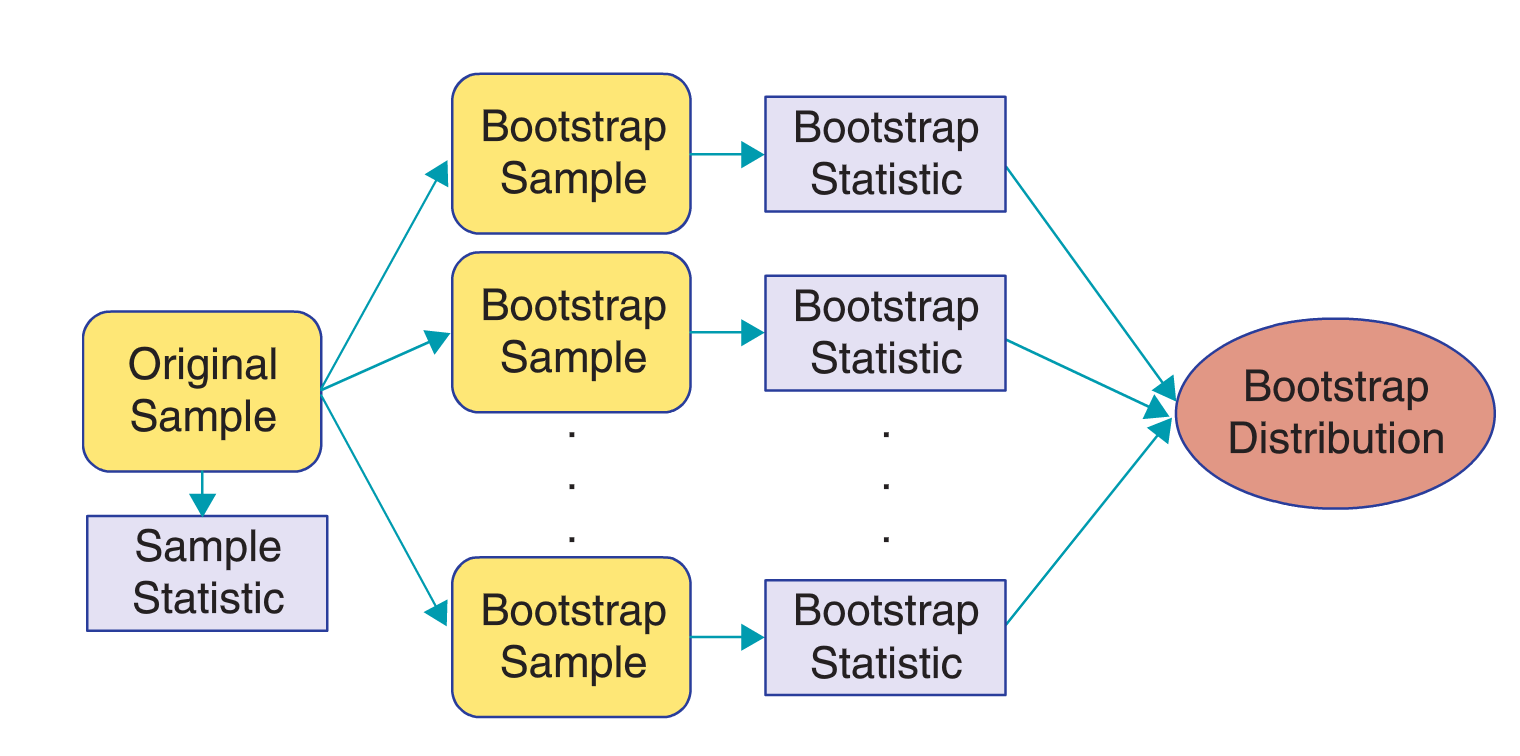
\includegraphics[width=\textwidth]{images/bootstrap} 

}

\caption[Bootstrapping diagram from Lock5 textbook]{Bootstrapping diagram from Lock5 textbook}\label{fig:bootstrapimg}
\end{figure}

\section{What's to come?}\label{whats-to-come-3}

This chapter has served as an introduction into inferential techniques
that will be discussed in greater detail in Chapter \ref{hypo} for
hypothesis testing and in Chapter \ref{ci} for confidence intervals. In
these chapters, we will see how we can use a related concept of
\textbf{resampling} when working with the distributions of two groups.
All of these concepts will be further reinforced in Chapter
\ref{regress} as well.

\chapter{Hypothesis Testing}\label{hypo}

We saw some of the main concepts of hypothesis testing introduced in
Chapter \ref{infer-basics}. We will expand further on these ideas here
and also provide a framework for understanding hypothesis tests in
general. Instead of presenting you with lots of different formulas and
scenarios, we hope to build a way to think about all hypothesis tests.
You can then adapt to different scenarios as needed down the road when
you encounter different statistical situations.

In a hypothesis test, we will use data from a sample to help us decide
between two competing \emph{hypotheses} about a population. We make
these hypotheses more concrete by specifying them in terms of at least
one \emph{population parameter} of interest. We refer to the competing
claims about the population as the \textbf{null hypothesis}, denoted by
\(H_0\), and the \textbf{alternative (or research) hypothesis}, denoted
by \(H_a\). The roles of these two hypotheses are NOT interchangeable.

\begin{itemize}
\tightlist
\item
  The claim for which we seek significant evidence is assigned to the
  alternative hypothesis. The alternative is usually what the
  experimenter or researcher wants to establish or find evidence for.
\item
  Usually, the null hypothesis is a claim that there really is ``no
  effect'' or ``no difference.'' In many cases, the null hypothesis
  represents the status quo or that nothing interesting is happening.\\
\item
  We assess the strength of evidence by assuming the null hypothesis is
  true and determining how unlikely it would be to see sample results as
  extreme (or more extreme) as those in the original sample.
\end{itemize}

Hypothesis testing brings about many weird and incorrect notions in the
scientific community and society at large. One reason for this is that
statistics has traditionally been thought of as this magic box of
algorithms and procedures to get to results and this has been readily
apparent if you do a Google search of ``flowchart statistics hypothesis
tests''. There are so many different complex ways to determine which
test is appropriate.

You'll see that we don't need to rely on these complicated series of
assumptions and procedures to conduct a hypothesis test any longer.
These methods were introduced in a time when computers weren't powerful.
Your cellphone (in 2016) has more power than the computers that sent
NASA astronauts to the moon after all. We'll see that ALL hypothesis
tests can be broken down into the following framework given by Allen
Downey
\href{http://allendowney.blogspot.com/2016/06/there-is-still-only-one-test.html}{here}:

\begin{figure}

{\centering 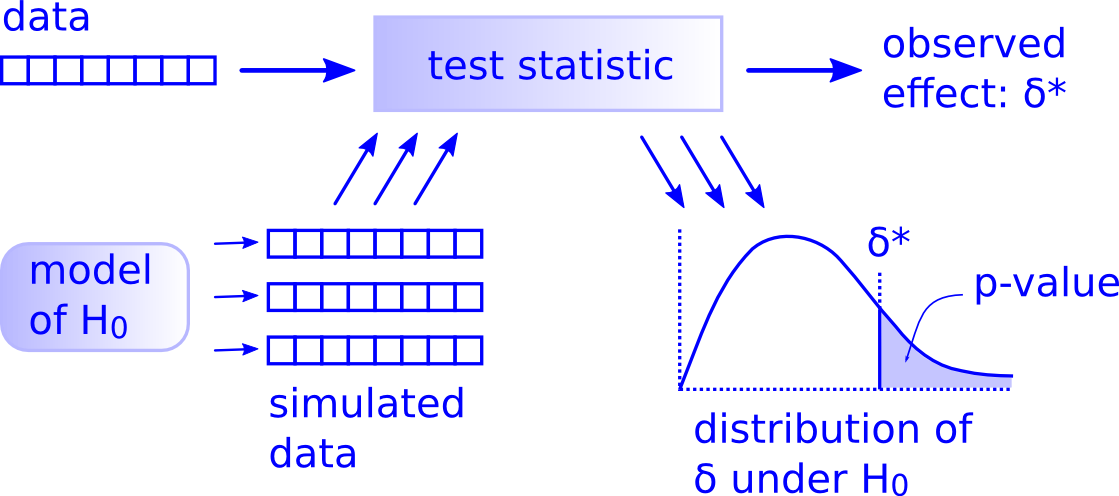
\includegraphics[width=\textwidth]{images/ht} 

}

\caption[Hypothesis Testing Framework]{Hypothesis Testing Framework}\label{fig:htdowney}
\end{figure}

Before we hop into this framework, we will provide another way to think
about hypothesis testing that may be useful.

\section{Criminal trial analogy}\label{trial}

We can think of hypothesis testing in the same context as a criminal
trial in the United States. A criminal trial in the United States is a
familiar situation in which a choice between two contradictory claims
must be made.

\begin{enumerate}
\def\labelenumi{\arabic{enumi}.}
\item
  The accuser of the crime must be judged either guilty or not guilty.
\item
  Under the U.S. system of justice, the individual on trial is initially
  presumed not guilty.
\item
  Only STRONG EVIDENCE to the contrary causes the not guilty claim to be
  rejected in favor of a guilty verdict.
\item
  The phrase ``beyond a reasonable doubt'' is often used to set the
  cutoff value for when enough evidence has been given to convict.
\end{enumerate}

Theoretically, we should never say ``The person is innocent.'' but
instead ``There is not sufficient evidence to show that the person is
guilty.''

Now let's compare that to how we look at a hypothesis test.

\begin{enumerate}
\def\labelenumi{\arabic{enumi}.}
\item
  The decision about the population parameter(s) must be judged to
  follow one of two hypotheses.
\item
  We initially assume that \(H_0\) is true.
\item
  The null hypothesis \(H_0\) will be rejected (in favor of \(H_a\))
  only if the sample evidence strongly suggests that \(H_0\) is false.
  If the sample does not provide such evidence, \(H_0\) will not be
  rejected.
\item
  The analogy to ``beyond a reasonable doubt'' in hypothesis testing is
  what is known as the \textbf{significance level}. This will be set
  before conducting the hypothesis test and is denoted as \(\alpha\).
  Common values for \(\alpha\) are 0.1, 0.01, and 0.05.
\end{enumerate}

\subsection{Two possible conclusions}\label{two-possible-conclusions}

Therefore, we have two possible conclusions with hypothesis testing:

\begin{itemize}
\tightlist
\item
  Reject \(H_0\)\\
\item
  Fail to reject \(H_0\)
\end{itemize}

Gut instinct says that ``Fail to reject \(H_0\)'' should say ``Accept
\(H_0\)'' but this technically is not correct. Accepting \(H_0\) is the
same as saying that a person is innocent. We cannot show that a person
is innocent; we can only say that there was not enough substantial
evidence to find the person guilty.

When you run a hypothesis test, you are the jury of the trial. You
decide whether there is enough evidence to convince yourself that
\(H_a\) is true (``the person is guilty'') or that there was not enough
evidence to convince yourself \(H_a\) is true (``the person is not
guilty''). You must convince yourself (using statistical arguments)
which hypothesis is the correct one given the sample information.

\textbf{Important note:} Therefore, DO NOT WRITE ``Accept \(H_0\)'' any
time you conduct a hypothesis test. Instead write ``Fail to reject
\(H_0\)''.

\subsection{Basic Logic of Hypothesis
Testing}\label{basic-logic-of-hypothesis-testing}

\begin{itemize}
\tightlist
\item
  Take a random sample (or samples) from a population (or two
  populations)
\item
  If the sample data are consistent with the null hypothesis, do not
  reject the null hypothesis.
\item
  If the sample data are inconsistent with the null hypothesis (in the
  direction of the alternative hypothesis), reject the null hypothesis
  and conclude that the alternative hypothesis is true (based on the
  particular sample collected).
\end{itemize}

\subsection{Statistical Significance}\label{statistical-significance}

The idea that sample results are more extreme than we would reasonably
expect to see by random chance if the null hypothesis were true is the
fundamental idea behind statistical hypothesis tests. If data as extreme
would be very unlikely if the null hypothesis were true, we say the data
are \textbf{statistically significant}. Statistically significant data
provide convincing evidence against the null hypothesis in favor of the
alternative, and allow us to generalize our sample results to the claim
about the population.

\begin{center}\rule{0.5\linewidth}{\linethickness}\end{center}

\textbf{Definition: Statistical Significance}

When results as extreme as the observed sample statistic are unlikely to
occur by random chance alone (assuming the null hypothesis is true), we
say the sample results are \emph{statistically significant}. If our
sample is statistically significant, we have convincing evidence against
\(H_0\) and in favor of \(H_a\). ***

\section{Randomization}\label{randomization}

We will now focus on building hypotheses looking at the difference
between two population means in an example. We will denote population
means using the Greek symbol \(\mu\) (pronounced ``mu''). Thus, we will
be looking to see if one group ``out-performs'' another group. This is
the quite possibly the most common type of statistical inference and
serves as a basis for many other types of analyses when comparing two
groups.

Our null hypothesis will be of the form \(H_0: \mu_1 = \mu_2\), which
can also be written as \(H_0: \mu_1 - \mu_2 = 0\). Our alternative
hypothesis will be of the form \(H_0: \mu_1 \star \mu_2\) (or
\(H_a: \mu_1 - \mu_2 \, \star \, 0\)) where \(\star\) = \(<\), \(\ne\),
or \(>\) depending on the context of the problem. You needn't focus on
these new symbols too much at this point. It will just be a shortcut way
for us to describe our hypotheses.

As we saw in Chapter \ref{infer-basics}, simulation and bootstrapping
are valuable tools when conducting inferences based on one population
variable. We will see that the process of \textbf{randomization}, which
is a resampling procedure similar to bootstrapping in some ways will be
valuable in conducting tests comparing quantitative values from two
groups.

\begin{center}\rule{0.5\linewidth}{\linethickness}\end{center}

\begin{learncheck}
\textbf{\emph{Learning check}}
\end{learncheck}

\textbf{(LC7.1)} What is wrong about saying ``The defendant is
innocent.'' based on the US system of criminal trials?

\textbf{(LC7.2)} What is the purpose of hypothesis testing?

\textbf{(LC7.3)} What are some flaws with hypothesis testing? How could
we alleviate them?

\begin{center}\rule{0.5\linewidth}{\linethickness}\end{center}

\subsection{Comparing Action and Romance
Movies}\label{comparing-action-and-romance-movies}

The \texttt{movies} data set in the \texttt{ggplot2movies} package
contains information on a large number of movies that have been rated by
users of IMDB.com. We are interested in the question here of whether
\texttt{Action} movies are rated higher on IMDB than \texttt{Romance}
movies. We will first need to do a little bit of data manipulation using
the ideas from Chapter \ref{manip} to get the data in the form that we
would like:

\begin{Shaded}
\begin{Highlighting}[]
\KeywordTok{library}\NormalTok{(dplyr)}
\KeywordTok{library}\NormalTok{(ggplot2movies)}
\NormalTok{movies_trimmed <-}\StringTok{ }\NormalTok{movies %>%}\StringTok{ }
\StringTok{  }\KeywordTok{select}\NormalTok{(title, year, rating, Action, Romance)}
\NormalTok{movies_trimmed}
\end{Highlighting}
\end{Shaded}

\begin{verbatim}
## # A tibble: 58,788 x 5
##                       title  year rating Action Romance
##                       <chr> <int>  <dbl>  <int>   <int>
## 1                         $  1971    6.4      0       0
## 2         $1000 a Touchdown  1939    6.0      0       0
## 3    $21 a Day Once a Month  1941    8.2      0       0
## 4                   $40,000  1996    8.2      0       0
## 5  $50,000 Climax Show, The  1975    3.4      0       0
## 6                     $pent  2000    4.3      0       0
## 7                   $windle  2002    5.3      1       0
## 8                      '15'  2002    6.7      0       0
## 9                       '38  1987    6.6      0       0
## 10                  '49-'17  1917    6.0      0       0
## # ... with 58,778 more rows
\end{verbatim}

Note that \texttt{Action} and \texttt{Romance} are binary variables
here. To remove any overlap of movies (and potential confusion) that are
both \texttt{Action} and \texttt{Romance}, we will remove them from our
\emph{population}:

\begin{Shaded}
\begin{Highlighting}[]
\NormalTok{movies_trimmed <-}\StringTok{ }\NormalTok{movies_trimmed %>%}
\StringTok{  }\KeywordTok{filter}\NormalTok{(!(Action ==}\StringTok{ }\DecValTok{1} \NormalTok{&}\StringTok{ }\NormalTok{Romance ==}\StringTok{ }\DecValTok{1}\NormalTok{))}
\end{Highlighting}
\end{Shaded}

We will now create a new variable called \texttt{genre} that specifies
whether a movie in our \texttt{movies\_trimmed} data frame is an
\texttt{"Action"} movie, a \texttt{"Romance"} movie, or
\texttt{"Neither"}. We aren't really interested in the
\texttt{"Neither"} category here so we will exclude those rows as well.
Lastly, the \texttt{Action} and \texttt{Romance} columns are not needed
anymore since they are encoded in the \texttt{genre} column.

\begin{Shaded}
\begin{Highlighting}[]
\NormalTok{movies_trimmed <-}\StringTok{ }\NormalTok{movies_trimmed %>%}
\StringTok{  }\KeywordTok{mutate}\NormalTok{(}\DataTypeTok{genre =} \KeywordTok{ifelse}\NormalTok{(Action ==}\StringTok{ }\DecValTok{1}\NormalTok{, }\StringTok{"Action"}\NormalTok{,}
                        \KeywordTok{ifelse}\NormalTok{(Romance ==}\StringTok{ }\DecValTok{1}\NormalTok{, }\StringTok{"Romance"}\NormalTok{,}
                               \StringTok{"Neither"}\NormalTok{))) %>%}
\StringTok{  }\KeywordTok{filter}\NormalTok{(genre !=}\StringTok{ "Neither"}\NormalTok{) %>%}
\StringTok{  }\KeywordTok{select}\NormalTok{(-Action, -Romance)}
\end{Highlighting}
\end{Shaded}

We are left with 8878 movies in our \emph{population} data set that
focuses on only \texttt{"Action"} and \texttt{"Romance"} movies.

\begin{center}\rule{0.5\linewidth}{\linethickness}\end{center}

\begin{learncheck}
\textbf{\emph{Learning check}}
\end{learncheck}

\textbf{(LC7.4)} Why are the different genre variables stored as binary
variables stored as 1s and 0s instead of just listing the genre as a
column of values like ``Action'', ``Comedy'', etc.?

\textbf{(LC7.5)} What complications could come above with us excluding
action romance movies? Should we question the results of our hypothesis
test? Explain.

\begin{center}\rule{0.5\linewidth}{\linethickness}\end{center}

Let's now visualize the distributions of \texttt{rating} across both
levels of \texttt{genre}. Think about what type(s) of plot is/are
appropriate here before you proceed:

\begin{Shaded}
\begin{Highlighting}[]
\KeywordTok{library}\NormalTok{(ggplot2)}
\NormalTok{movies_trimmed %>%}\StringTok{ }\KeywordTok{ggplot}\NormalTok{(}\KeywordTok{aes}\NormalTok{(}\DataTypeTok{x =} \NormalTok{genre, }\DataTypeTok{y =} \NormalTok{rating)) +}
\StringTok{  }\KeywordTok{geom_boxplot}\NormalTok{()}
\end{Highlighting}
\end{Shaded}

\begin{figure}

{\centering 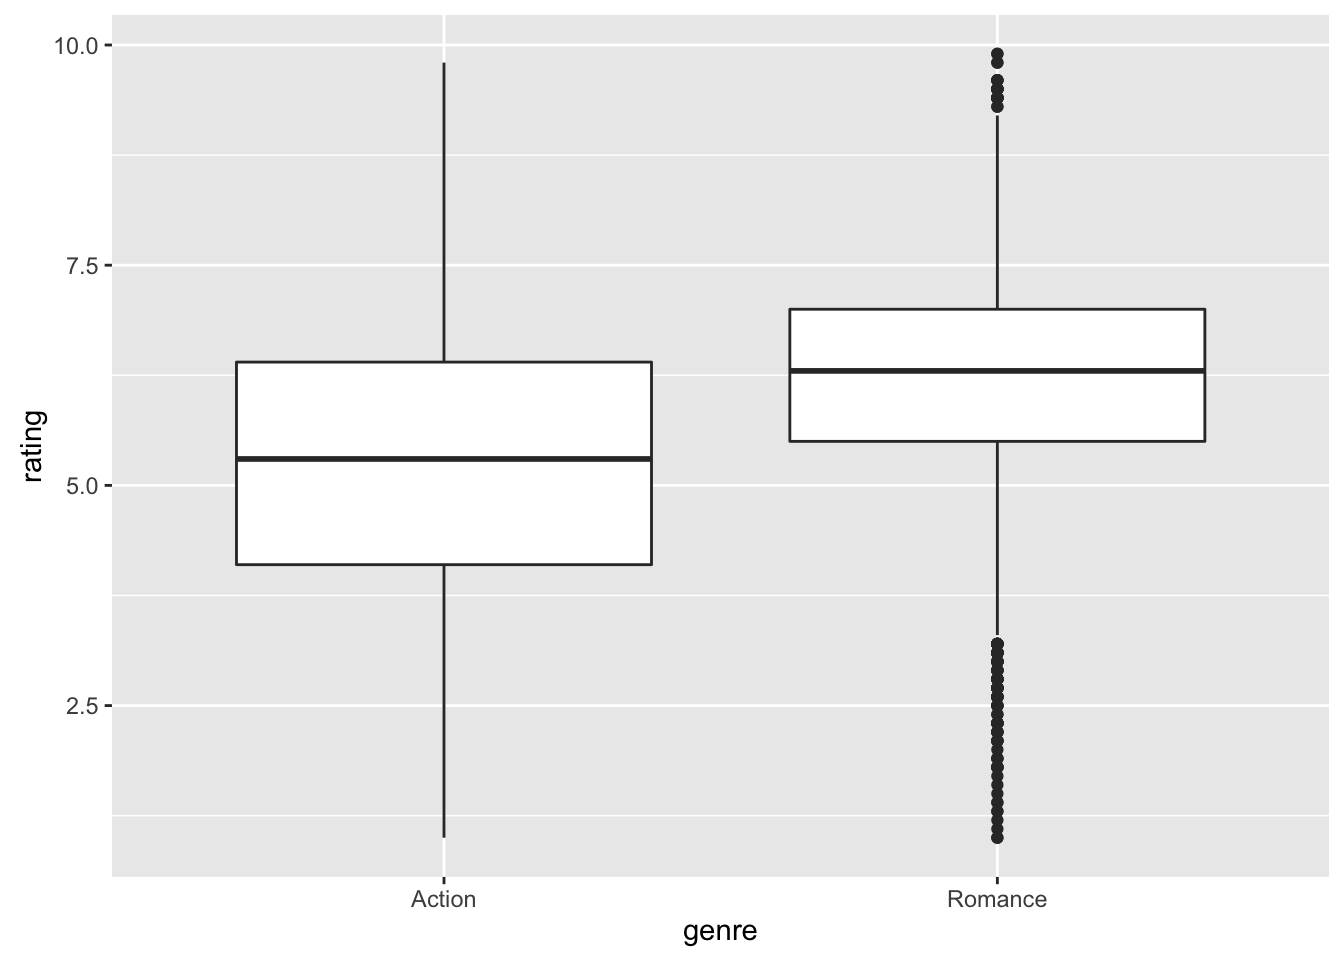
\includegraphics[width=\textwidth]{ismay_files/figure-latex/unnamed-chunk-97-1} 

}

\caption[Rating vs genre in the population]{Rating vs genre in the population}\label{fig:unnamed-chunk-97}
\end{figure}

We can see that the middle 50\% of ratings for \texttt{"Action"} movies
is more spread out than that of \texttt{"Romance"} movies in the
population. \texttt{Romance} has outliers at both the top and bottoms of
the scale though. We are initially interested in comparing the mean
\texttt{rating} across these two groups so a faceted histogram may also
be useful:

\begin{Shaded}
\begin{Highlighting}[]
\NormalTok{movies_trimmed %>%}\StringTok{ }\KeywordTok{ggplot}\NormalTok{(}\DataTypeTok{mapping =} \KeywordTok{aes}\NormalTok{(}\DataTypeTok{x =} \NormalTok{rating)) +}
\StringTok{  }\KeywordTok{geom_histogram}\NormalTok{(}\DataTypeTok{binwidth =} \DecValTok{1}\NormalTok{, }\DataTypeTok{color =} \StringTok{"white"}\NormalTok{, }\DataTypeTok{fill =} \StringTok{"dodgerblue"}\NormalTok{) +}
\StringTok{  }\KeywordTok{facet_wrap}\NormalTok{(~genre)}
\end{Highlighting}
\end{Shaded}

\begin{figure}

{\centering 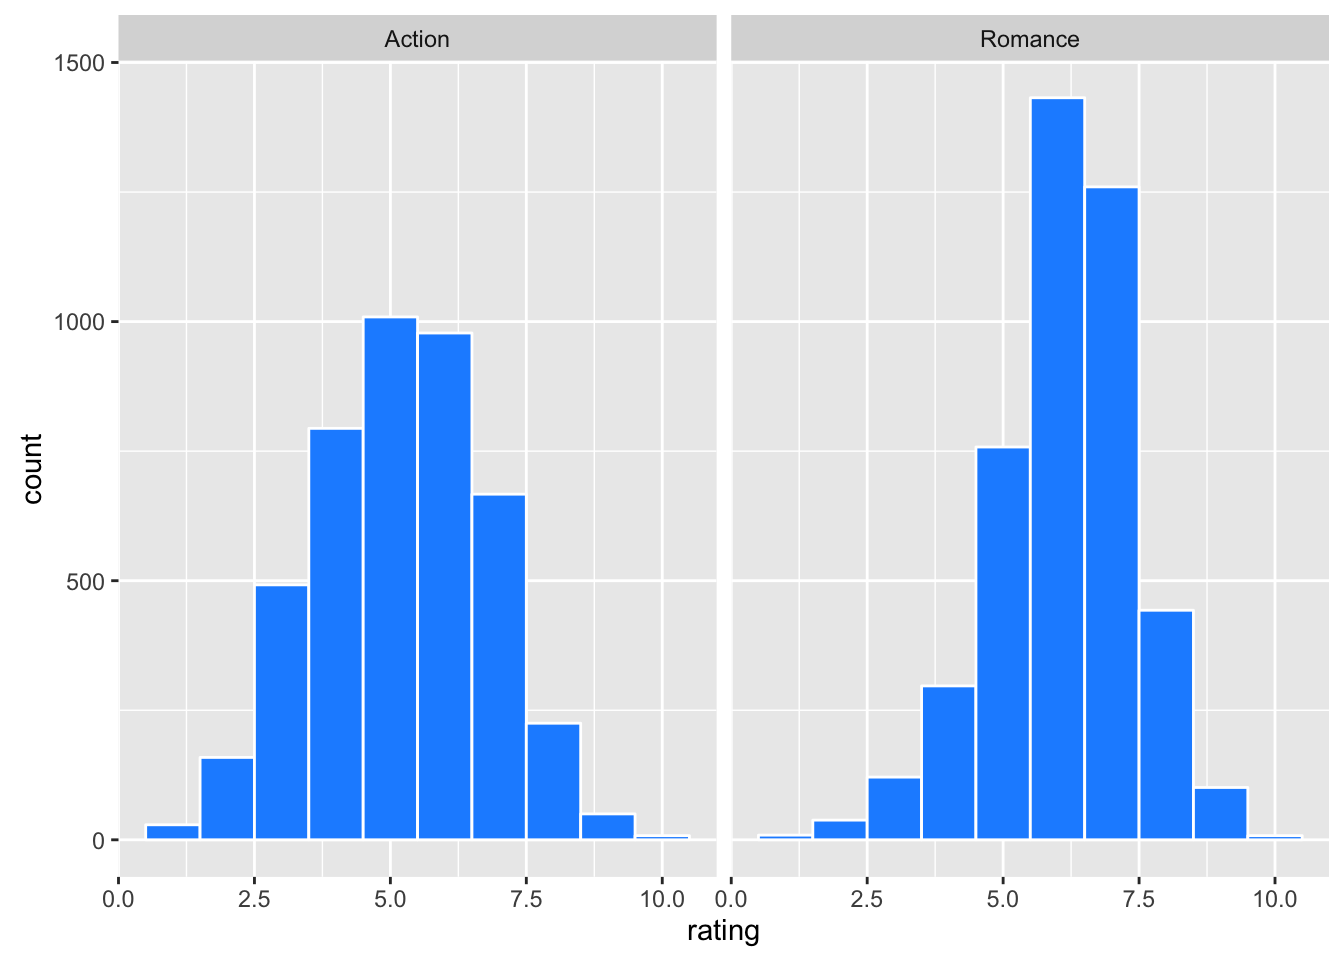
\includegraphics[width=\textwidth]{ismay_files/figure-latex/unnamed-chunk-98-1} 

}

\caption[Faceted histogram of genre vs rating]{Faceted histogram of genre vs rating}\label{fig:unnamed-chunk-98}
\end{figure}

\textbf{Important note:} Remember that we hardly ever have access to the
population values as we do here. This example and the
\texttt{nycflights13} data set were used to create a common flow from
chapter to chapter. In nearly all circumstances, we'll be needing to use
only a sample of the population to try to infer conclusions about the
unknown population parameter values. These examples do show a nice
relationship between statistics (where data is usually small and more
focused on experimental settings) and data science (where data is
frequently large and collected without experimental conditions). We'll
learn more about observational studies and experiments in Chapter
\ref{regress}.

\subsection{Sampling -\textgreater{}
Randomization}\label{sampling---randomization}

We can use hypothesis testing to investigate ways to determine, for
example, whether a \textbf{treatment} has an effect over a
\textbf{control} and other ways to statistically analyze if one group
performs better than, worse than, or different than another. We will
also use confidence intervals to determine the size of the effect if it
exists. You'll see more on this in Chapter \ref{ci}.

We are interested here in seeing how we can use a random sample of
action movies and a random sample of romance movies from \texttt{movies}
to determine if a statistical difference exists in the mean ratings of
each group.

\begin{center}\rule{0.5\linewidth}{\linethickness}\end{center}

\begin{learncheck}
\textbf{\emph{Learning check}}
\end{learncheck}

\textbf{(LC7.6)} Define the relevant parameters here in terms of the
populations of movies.

\begin{center}\rule{0.5\linewidth}{\linethickness}\end{center}

Let's select a random sample of 34 action movies and a random sample of
34 romance movies. (The number 34 was chosen somewhat arbitrarily here.)

\begin{Shaded}
\begin{Highlighting}[]
\KeywordTok{library}\NormalTok{(dplyr)}
\KeywordTok{set.seed}\NormalTok{(}\DecValTok{2016}\NormalTok{)}
\NormalTok{movies_genre_sample <-}\StringTok{ }\NormalTok{movies_trimmed %>%}\StringTok{ }
\StringTok{  }\KeywordTok{group_by}\NormalTok{(genre) %>%}
\StringTok{  }\KeywordTok{sample_n}\NormalTok{(}\DecValTok{34}\NormalTok{)}
\end{Highlighting}
\end{Shaded}

We can now observe the distributions of our two sample ratings for both
groups. Remember that these plots should be rough approximations of our
population distributions.

\begin{Shaded}
\begin{Highlighting}[]
\NormalTok{movies_genre_sample %>%}\StringTok{ }\KeywordTok{ggplot}\NormalTok{(}\KeywordTok{aes}\NormalTok{(}\DataTypeTok{x =} \NormalTok{genre, }\DataTypeTok{y =} \NormalTok{rating)) +}
\StringTok{  }\KeywordTok{geom_boxplot}\NormalTok{()}
\end{Highlighting}
\end{Shaded}

\begin{figure}

{\centering 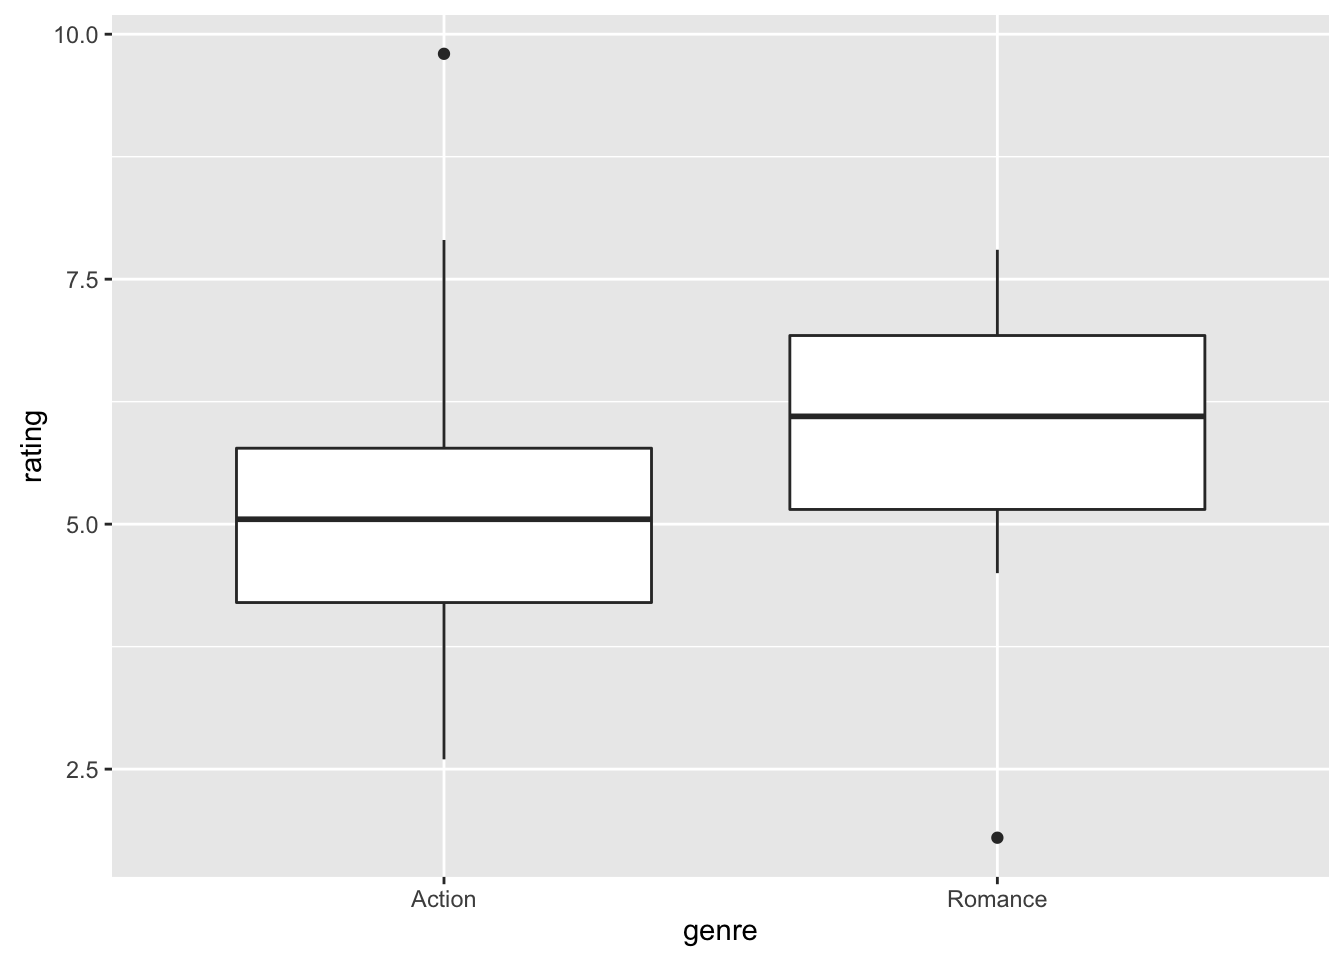
\includegraphics[width=\textwidth]{ismay_files/figure-latex/unnamed-chunk-100-1} 

}

\caption[Genre vs rating for our sample]{Genre vs rating for our sample}\label{fig:unnamed-chunk-100}
\end{figure}

\begin{Shaded}
\begin{Highlighting}[]
\NormalTok{movies_genre_sample %>%}\StringTok{ }\KeywordTok{ggplot}\NormalTok{(}\DataTypeTok{mapping =} \KeywordTok{aes}\NormalTok{(}\DataTypeTok{x =} \NormalTok{rating)) +}
\StringTok{  }\KeywordTok{geom_histogram}\NormalTok{(}\DataTypeTok{binwidth =} \DecValTok{1}\NormalTok{, }\DataTypeTok{color =} \StringTok{"white"}\NormalTok{, }\DataTypeTok{fill =} \StringTok{"dodgerblue"}\NormalTok{) +}
\StringTok{  }\KeywordTok{facet_wrap}\NormalTok{(~genre)}
\end{Highlighting}
\end{Shaded}

\begin{figure}

{\centering 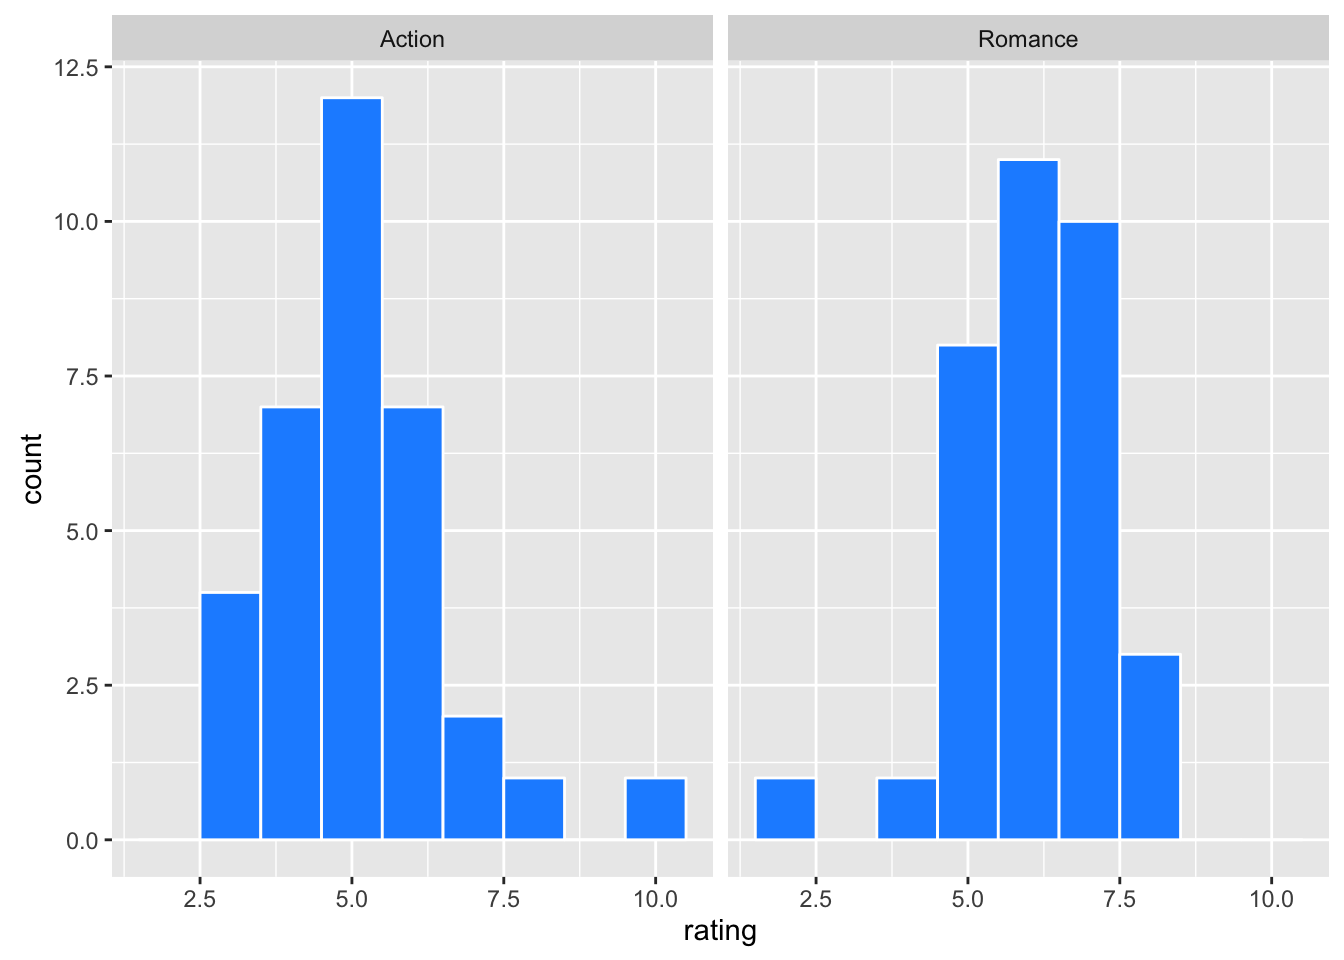
\includegraphics[width=\textwidth]{ismay_files/figure-latex/unnamed-chunk-101-1} 

}

\caption[Genre vs rating for our sample as faceted histogram]{Genre vs rating for our sample as faceted histogram}\label{fig:unnamed-chunk-101}
\end{figure}

\begin{center}\rule{0.5\linewidth}{\linethickness}\end{center}

\begin{learncheck}
\textbf{\emph{Learning check}}
\end{learncheck}

\textbf{(LC7.7)} What single value could we change to improve the
approximation using the sample distribution on the population
distribution?

\begin{center}\rule{0.5\linewidth}{\linethickness}\end{center}

Do we have reason to believe, based on the sample distributions of
\texttt{rating} over the two groups of \texttt{genre}, that there is a
significant difference between the mean \texttt{rating} for action
movies compared to romance movies? It's hard to say just based on the
plots. The boxplot does show that the median sample rating is higher
romance movies, but the histogram isn't as clear. The two groups have
somewhat differently shaped distributions but they are both over similar
values of \texttt{rating}. It's often useful to calculate the mean and
standard deviation as well conditioned on the two levels.

\begin{Shaded}
\begin{Highlighting}[]
\NormalTok{summary_ratings <-}\StringTok{ }\NormalTok{movies_genre_sample %>%}\StringTok{ }\KeywordTok{group_by}\NormalTok{(genre) %>%}
\StringTok{  }\KeywordTok{summarize}\NormalTok{(}\DataTypeTok{mean =} \KeywordTok{mean}\NormalTok{(rating),}
            \DataTypeTok{std_dev =} \KeywordTok{sd}\NormalTok{(rating))}
\NormalTok{summary_ratings}
\end{Highlighting}
\end{Shaded}

\begin{verbatim}
## # A tibble: 2 x 3
##     genre     mean  std_dev
##     <chr>    <dbl>    <dbl>
## 1  Action 5.197059 1.464837
## 2 Romance 6.026471 1.202096
\end{verbatim}

\begin{center}\rule{0.5\linewidth}{\linethickness}\end{center}

\begin{learncheck}
\textbf{\emph{Learning check}}
\end{learncheck}

\textbf{(LC7.8)} Why did we not specify \texttt{na.rm\ =\ TRUE} here as
we did in Chapter \ref{manip}?

\begin{center}\rule{0.5\linewidth}{\linethickness}\end{center}

We see that the sample mean rating for romance movies, \(\bar{x}_{r}\),
is greater than the similar measure for action movies, \(\bar{x}_a\).
But is it statistically significantly greater (thus, leading us to
conclude that the means are statistically different)? The standard
deviation can provide some insight here but with these standard
deviations being so similar it's still hard to say for sure.

\begin{center}\rule{0.5\linewidth}{\linethickness}\end{center}

\begin{learncheck}
\textbf{\emph{Learning check}}
\end{learncheck}

\textbf{(LC7.9)} Why might the standard deviation provide some insight
about the means being statistically different or not?

\begin{center}\rule{0.5\linewidth}{\linethickness}\end{center}

The hypotheses we specified can also be written in another form to
better give us an idea of what we will be simulating to create our null
distribution.

\begin{itemize}
\tightlist
\item
  \(H_0: \mu_r - \mu_a = 0\)
\item
  \(H_a: \mu_r - \mu_a \ne 0\)
\end{itemize}

We are, therefore, interested in seeing whether the difference in the
sample means, \(\bar{x}_r - \bar{x}_a\), is statistically different than
0. R has a built-in command that can calculate the difference in these
two sample means.

\begin{Shaded}
\begin{Highlighting}[]
\NormalTok{mean_ratings <-}\StringTok{ }\NormalTok{movies_genre_sample %>%}\StringTok{ }\KeywordTok{group_by}\NormalTok{(genre) %>%}
\StringTok{  }\KeywordTok{summarize}\NormalTok{(}\DataTypeTok{mean =} \KeywordTok{mean}\NormalTok{(rating))}
\NormalTok{obs_diff <-}\StringTok{ }\KeywordTok{diff}\NormalTok{(mean_ratings$mean)}
\end{Highlighting}
\end{Shaded}

We see here that the \texttt{diff} function calculates
\(\bar{x}_r - \bar{x}_a = 6.0264706 - 5.1970588 = 0.8294118\). We will
now proceed similarly to how we conducted hypothesis tests in Chapter
\ref{infer-basics} using simulation. We can look at this from a tactile
point of view by using index cards. There are \(n_r = 34\) data elements
corresponding to romance movies and \(n_a = 34\) for action movies. We
can write the 34 ratings from our sample for romance movies on one set
of 34 index cards and the 34 leniency scores for action movies on
another set of 34 index cards. (Note that the sample sizes need not be
the same.)

The next step is to put the two stacks of index cards together, creating
a new set of 68 cards. If we assume that the two population means are
equal, we are saying that there is no association between ratings and
genre (romance vs action). We can use the index cards to create two
\textbf{new} stacks for romance and action movies. First, we must
shuffle all the cards thoroughly. After doing so, in this case with
equal values of sample sizes, we split the deck in half.

We then calculate the new sample mean rating of the romance deck, and
also the new sample mean rating of the action deck. This creates one
simulation of the samples. We next want to calculate a statistic from
these two samples. Instead of actually doing the calculation using index
cards, we can use R as we have before to simulate this process.

\begin{center}\rule{0.5\linewidth}{\linethickness}\end{center}

\begin{learncheck}
\textbf{\emph{Learning check}}
\end{learncheck}

\textbf{(LC7.10)} How would the tactile shuffling of index cards change
if we had different samples of say 20 action movies and 60 romance
movies? Describe each step that would change.

\textbf{(LC7.11)} Why are we taking the difference in the means of the
cards in the new shuffled decks?

\begin{center}\rule{0.5\linewidth}{\linethickness}\end{center}

\begin{Shaded}
\begin{Highlighting}[]
\KeywordTok{library}\NormalTok{(mosaic)}
\NormalTok{shuffled_ratings <-}\StringTok{ }\NormalTok{movies_trimmed %>%}
\StringTok{     }\KeywordTok{mutate}\NormalTok{(}\DataTypeTok{rating =} \KeywordTok{shuffle}\NormalTok{(rating)) %>%}\StringTok{ }
\StringTok{     }\KeywordTok{group_by}\NormalTok{(genre) %>%}
\StringTok{     }\KeywordTok{summarize}\NormalTok{(}\DataTypeTok{mean =} \KeywordTok{mean}\NormalTok{(rating))}
\KeywordTok{diff}\NormalTok{(shuffled_ratings$mean)}
\end{Highlighting}
\end{Shaded}

\begin{verbatim}
## [1] -0.02287811
\end{verbatim}

The only new command here is \texttt{shuffle} from the \texttt{mosaic}
package, which does what we would expect it to do. It simulates a
shuffling of the ratings between the two levels of \texttt{genre} just
as we could have done with index cards. We can now proceed in a similar
way to what we have done previously in Chapter \ref{infer-basics} by
repeating this process many times to create a \emph{null distribution}
of simulated differences in sample means.

\begin{Shaded}
\begin{Highlighting}[]
\NormalTok{many_shuffles <-}\StringTok{ }\KeywordTok{do}\NormalTok{(}\DecValTok{10000}\NormalTok{) *}\StringTok{ }
\StringTok{  }\NormalTok{(movies_trimmed %>%}
\StringTok{     }\KeywordTok{mutate}\NormalTok{(}\DataTypeTok{rating =} \KeywordTok{shuffle}\NormalTok{(rating)) %>%}\StringTok{ }
\StringTok{     }\KeywordTok{group_by}\NormalTok{(genre) %>%}
\StringTok{     }\KeywordTok{summarize}\NormalTok{(}\DataTypeTok{mean =} \KeywordTok{mean}\NormalTok{(rating))}
   \NormalTok{)}
\end{Highlighting}
\end{Shaded}

It is a good idea here to \texttt{View} the \texttt{many\_shuffles} data
frame via \texttt{View(many\_shuffles)}. We need to figure out a way to
subtract the first value of \texttt{mean} from the second value of
\texttt{mean} for each of the 10,000 simulations. This is a little
tricky but the \texttt{group\_by} function comes to our rescue here:

\begin{Shaded}
\begin{Highlighting}[]
\NormalTok{rand_distn <-}\StringTok{ }\NormalTok{many_shuffles %>%}
\StringTok{  }\KeywordTok{group_by}\NormalTok{(.index) %>%}
\StringTok{  }\KeywordTok{summarize}\NormalTok{(}\DataTypeTok{diffmean =} \KeywordTok{diff}\NormalTok{(mean))}
\end{Highlighting}
\end{Shaded}

We can now plot the distribution of these simulated differences in
means:

\begin{Shaded}
\begin{Highlighting}[]
\NormalTok{rand_distn %>%}\StringTok{ }\KeywordTok{ggplot}\NormalTok{(}\KeywordTok{aes}\NormalTok{(}\DataTypeTok{x =} \NormalTok{diffmean)) +}
\StringTok{  }\KeywordTok{geom_histogram}\NormalTok{(}\DataTypeTok{color =} \StringTok{"white"}\NormalTok{, }\DataTypeTok{bins =} \DecValTok{20}\NormalTok{)}
\end{Highlighting}
\end{Shaded}

\begin{figure}

{\centering 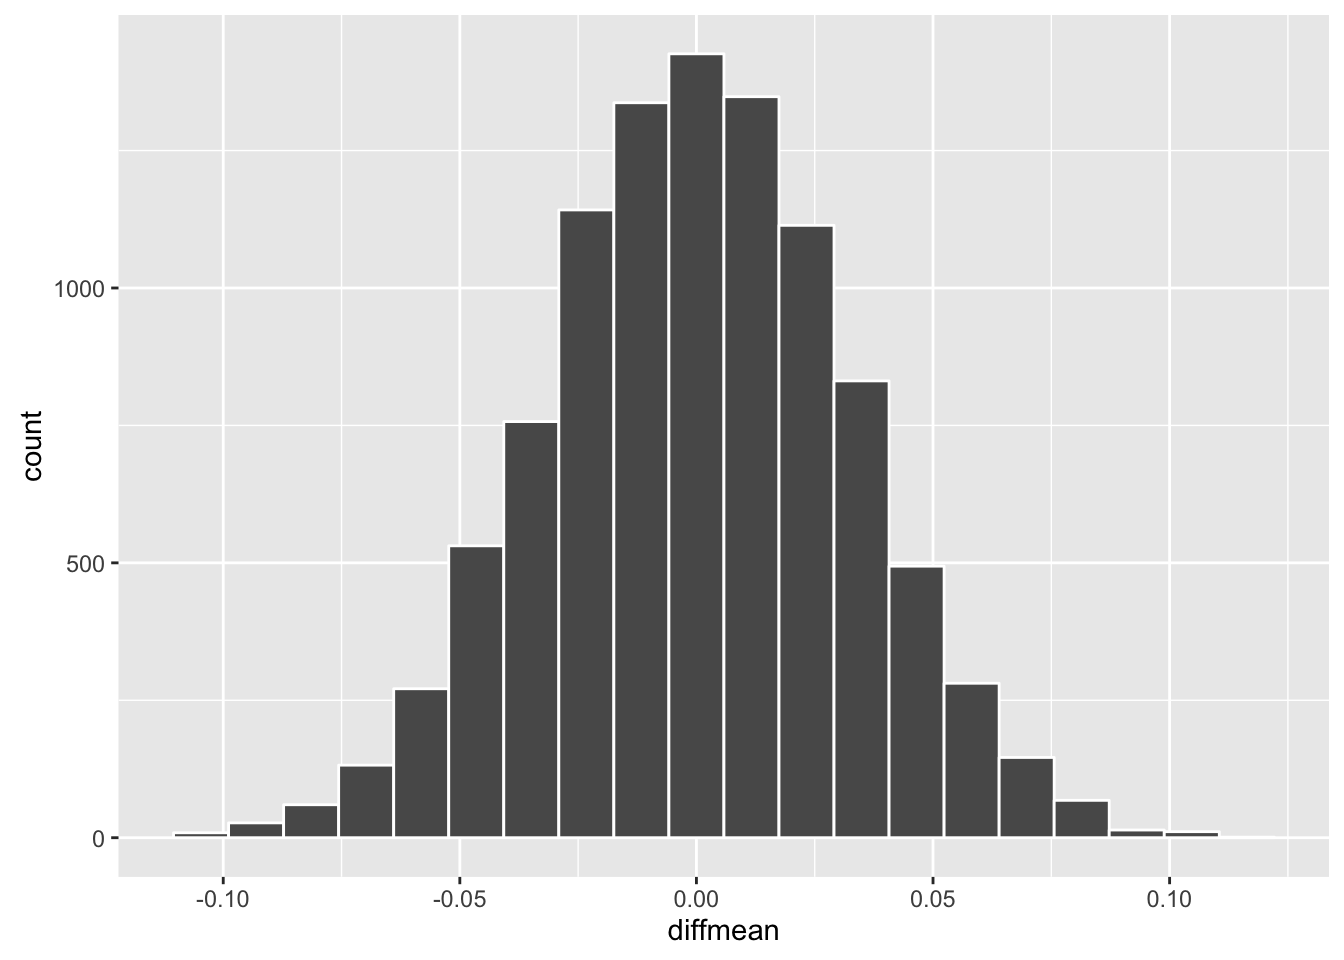
\includegraphics[width=\textwidth]{ismay_files/figure-latex/unnamed-chunk-107-1} 

}

\caption[Simulated differences in means histogram]{Simulated differences in means histogram}\label{fig:unnamed-chunk-107}
\end{figure}

Remember that we are interested in seeing where our observed sample mean
difference of 0.8294118 falls on this null distribution. We are
interested in simply a difference here so ``more extreme'' corresponds
to values in both tails on the distribution. Let's shade our null
distribution to show a visual representation of our \(p\)-value:

\begin{Shaded}
\begin{Highlighting}[]
\NormalTok{rand_distn %>%}\StringTok{ }\KeywordTok{ggplot}\NormalTok{(}\KeywordTok{aes}\NormalTok{(}\DataTypeTok{x =} \NormalTok{diffmean, }\DataTypeTok{fill =} \NormalTok{(}\KeywordTok{abs}\NormalTok{(diffmean) >=}\StringTok{ }\NormalTok{obs_diff))) +}
\StringTok{  }\KeywordTok{geom_histogram}\NormalTok{(}\DataTypeTok{color =} \StringTok{"white"}\NormalTok{, }\DataTypeTok{bins =} \DecValTok{20}\NormalTok{)}
\end{Highlighting}
\end{Shaded}

\begin{figure}

{\centering 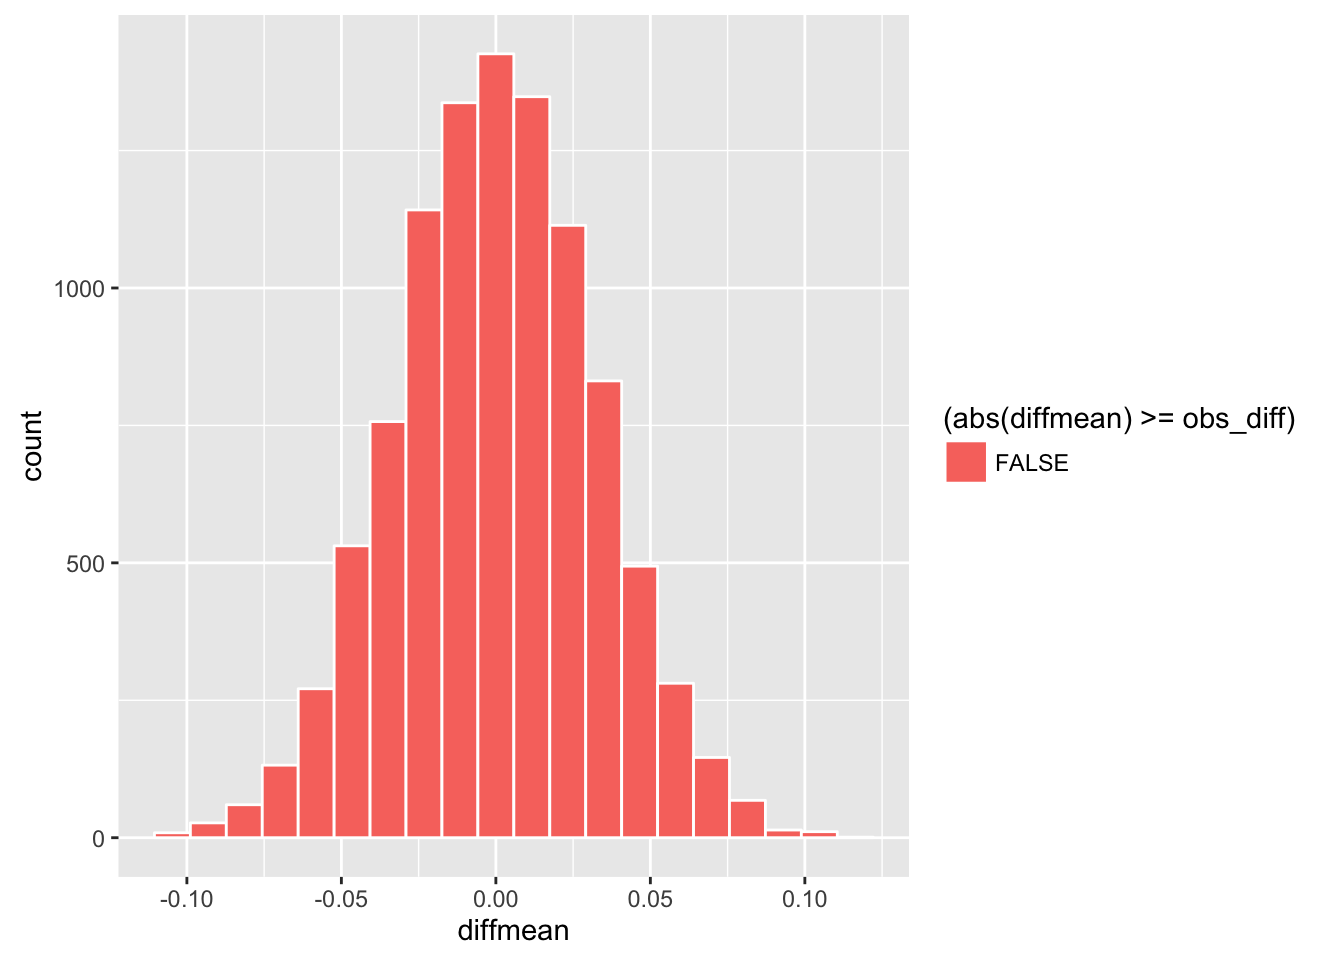
\includegraphics[width=\textwidth]{ismay_files/figure-latex/unnamed-chunk-108-1} 

}

\caption[Shaded histogram to show p-value]{Shaded histogram to show p-value}\label{fig:unnamed-chunk-108}
\end{figure}

You may initially think there is an error here, but remember that the
observed difference in means was 0.8294118. It falls far outside the
range of simulated differences. We can add a vertical line to represent
both it and its negative (since this is a two-tailed test) instead:

\begin{Shaded}
\begin{Highlighting}[]
\NormalTok{rand_distn %>%}\StringTok{ }\KeywordTok{ggplot}\NormalTok{(}\KeywordTok{aes}\NormalTok{(}\DataTypeTok{x =} \NormalTok{diffmean)) +}
\StringTok{  }\KeywordTok{geom_histogram}\NormalTok{(}\DataTypeTok{color =} \StringTok{"white"}\NormalTok{, }\DataTypeTok{bins =} \DecValTok{100}\NormalTok{) +}
\StringTok{  }\KeywordTok{geom_vline}\NormalTok{(}\DataTypeTok{xintercept =} \NormalTok{obs_diff, }\DataTypeTok{color =} \StringTok{"red"}\NormalTok{) +}
\StringTok{  }\KeywordTok{geom_vline}\NormalTok{(}\DataTypeTok{xintercept =} \NormalTok{-obs_diff, }\DataTypeTok{color =} \StringTok{"red"}\NormalTok{)}
\end{Highlighting}
\end{Shaded}

\begin{figure}

{\centering 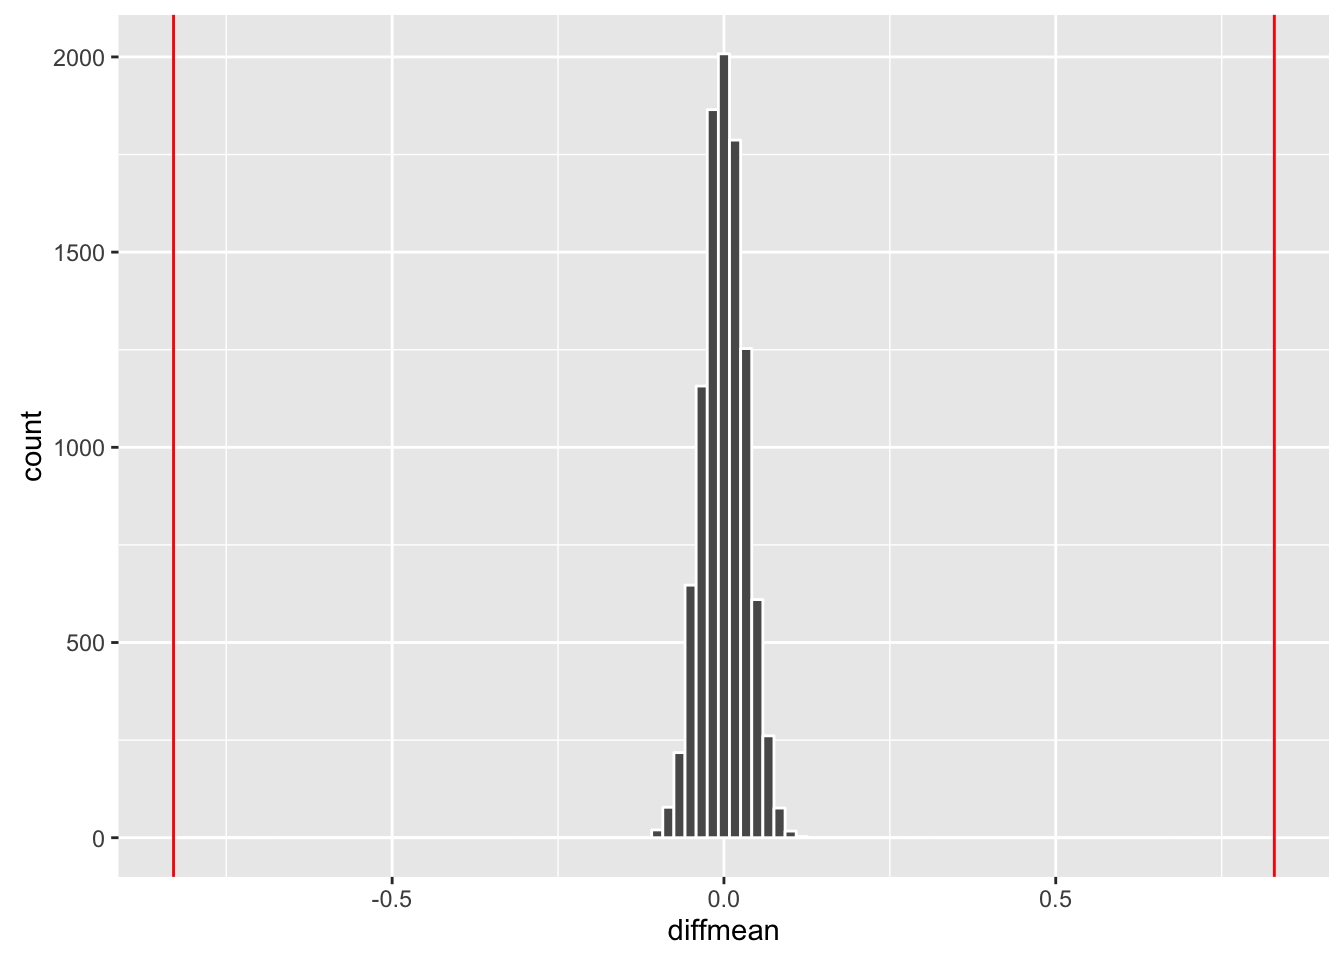
\includegraphics[width=\textwidth]{ismay_files/figure-latex/unnamed-chunk-109-1} 

}

\caption[Histogram with vertical lines corresponding to observed statistic]{Histogram with vertical lines corresponding to observed statistic}\label{fig:unnamed-chunk-109}
\end{figure}

Based on this plot, we have evidence supporting the conclusion that the
mean rating for romance movies is different from that of action movies.
(It doesn't really matter what significance level was chosen in this
case. Think about why.) The next important idea is to better understand
just how much higher of a mean rating can we expect the romance movies
to have compared to that of action movies. This can be addressed by
creating a 95\% confidence interval as we will explore in Chapter
\ref{ci}.

\begin{center}\rule{0.5\linewidth}{\linethickness}\end{center}

\begin{learncheck}
\textbf{\emph{Learning check}}
\end{learncheck}

\textbf{(LC7.12)} Conduct the same analysis comparing action movies
versus romantic movies using the median rating instead of the mean
rating? Make sure to use the \texttt{\%\textgreater{}\%} as much as
possible. What was different and what was the same?

\textbf{(LC7.13)} What conclusions can you make from viewing the faceted
histogram looking at \texttt{rating} versus \texttt{genre} that you
couldn't see when looking at the boxplot?

\textbf{(LC7.14)} Describe in a paragraph how we used Allen Downey's
diagram to conclude if a statistical difference existed between mean
movie ratings for action and romance movies.

\textbf{(LC7.15)} Why are we relatively confident that the distributions
of the sample ratings will be good approximations of the population
distributions of ratings for the two genres?

\textbf{(LC7.16)} What is the value of the \(p\)-value for the
hypothesis test comparing the mean rating of romance to action movies?

\textbf{(LC7.17)} Do the results of the hypothesis test match up with
the original plots we made looking at the population of movies? Why or
why not?

\begin{center}\rule{0.5\linewidth}{\linethickness}\end{center}

\subsection{Summary}\label{summary-5}

To review, these are the steps one would take whenever you'd like to do
a hypothesis test comparing values from the distributions of two groups:

\begin{itemize}
\item
  Simulate many samples using a random process that matches the way the
  original data were collected and that \emph{assumes the null
  hypothesis is true}.
\item
  Collect the values of a sample statistic for each sample to create a
  \emph{randomization distribution}.
\item
  Assess the significance of the \emph{original} sample by determining
  where its sample statistic lies in the randomization distribution.
\item
  If the proportion of values as extreme or more extreme than the
  observed statistic in the randomization distribution is smaller than
  the pre-determined significance level \(\alpha\), we reject \(H_0\).
  Otherwise, we fail to reject \(H_0\). (If no significance level is
  given, one can assume \(\alpha = 0.05\).)
\end{itemize}

\section{What's to come?}\label{whats-to-come-4}

This chapter examined how to conclude whether two sample statistics are
statistically different. This is the same thing as trying to conclude if
the difference in sample statistics is statistically different from
zero. We will see that this value of zero plays an important role in
confidence intervals as well. We'll also see in Chapter \ref{ci} the
relationship between confidence intervals and two-sided hypothesis tests
as we worked with in this chapter.

\chapter{Confidence Intervals}\label{ci}

\textbf{Definition: Confidence Interval}

A \emph{confidence interval} gives a range of plausible values for a
parameter. It depends on a specified \emph{confidence level} with higher
confidence levels corresponding to wider confidence intervals and lower
confidence levels corresponding to narrower confidence intervals. Common
confidence levels include 90\%, 95\%, and 99\%.

\section{Relation to hypothesis
testing}\label{relation-to-hypothesis-testing}

Recall that we found a statistically significant difference in the
sample mean of romance movie ratings compared to the sample mean of
action movie ratings. We concluded Chapter \ref{hypo} by attempted to
understand just how much greater we could expect the \emph{population}
mean romance movie rating to be as compared to the \emph{population}
mean action movie rating. In order to do so, we will calculate a
confidence interval for the difference \(\mu_r - \mu_a\). We'll then go
back to our population parameter values and see if our confidence
interval contains our parameter value.

We could use bootstrapping in a way similar to that done in the Chapter
\ref{infer-basics}, except now on a difference in sample means, to
create a distribution and then use the \texttt{confint} function with
the option of \texttt{quantile} to determine a confidence interval for
the plausible values of the difference in population means. This is an
excellent programming activity and the reader is urged to try to do so.

Recall what the randomization/null distribution looked like for our
simulated shuffled sample means:

\begin{Shaded}
\begin{Highlighting}[]
\KeywordTok{library}\NormalTok{(ggplot2)}
\KeywordTok{library}\NormalTok{(dplyr)}
\NormalTok{rand_distn %>%}\StringTok{ }\KeywordTok{ggplot}\NormalTok{(}\KeywordTok{aes}\NormalTok{(}\DataTypeTok{x =} \NormalTok{diffmean)) +}
\StringTok{  }\KeywordTok{geom_histogram}\NormalTok{(}\DataTypeTok{color =} \StringTok{"white"}\NormalTok{, }\DataTypeTok{bins =} \DecValTok{20}\NormalTok{)}
\end{Highlighting}
\end{Shaded}

\begin{figure}

{\centering 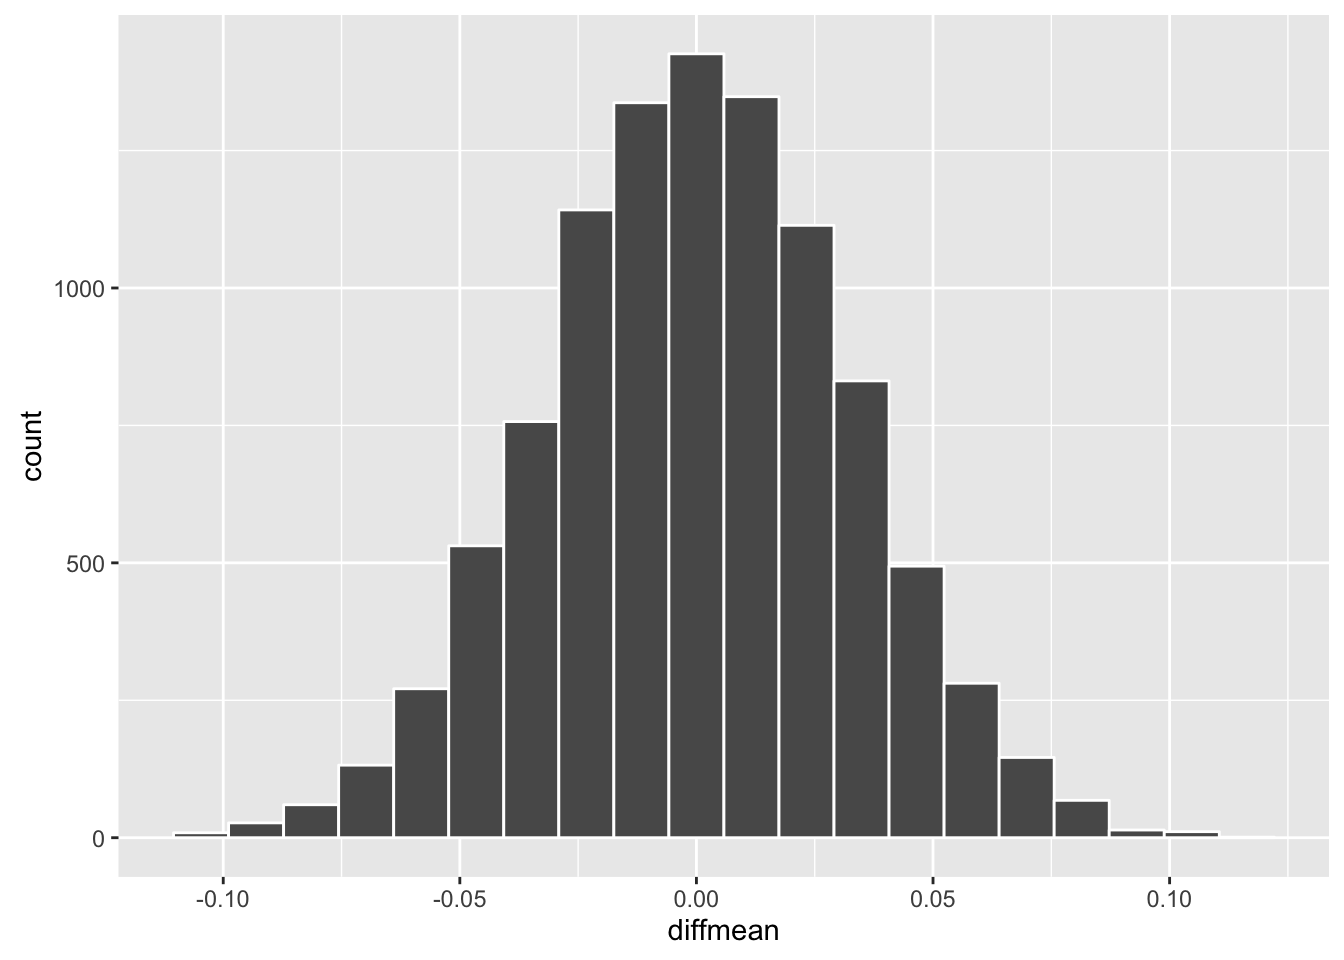
\includegraphics[width=\textwidth]{ismay_files/figure-latex/unnamed-chunk-110-1} 

}

\caption[Simulated shuffled sample means histogram]{Simulated shuffled sample means histogram}\label{fig:unnamed-chunk-110}
\end{figure}

With this null distribution being quite symmetric, the standard error
method introduced in Chapter \ref{infer-basics} likely provides a good
estimate of a range of plausible values for \(\mu_r - \mu_a\). Another
nice option here is that we can use the standard deviation of the
null/randomization distribution we just found with our hypothesis test.

\begin{Shaded}
\begin{Highlighting}[]
\NormalTok{(std_err <-}\StringTok{ }\NormalTok{rand_distn %>%}\StringTok{ }\KeywordTok{summarize}\NormalTok{(}\KeywordTok{sd}\NormalTok{(diffmean)))}
\end{Highlighting}
\end{Shaded}

\begin{verbatim}
## # A tibble: 1 x 1
##   sd(diffmean)
##          <dbl>
## 1   0.03208171
\end{verbatim}

Remembering that we can use the general formula of
\(statistic \pm (2 * SE)\) we get the following result for plausible
values of the difference in population means at the 95\% level.

\begin{Shaded}
\begin{Highlighting}[]
\NormalTok{(lower <-}\StringTok{ }\NormalTok{obs_diff -}\StringTok{ }\NormalTok{(}\DecValTok{2} \NormalTok{*}\StringTok{ }\NormalTok{std_err))}
\end{Highlighting}
\end{Shaded}

\begin{verbatim}
##   sd(diffmean)
## 1    0.7652483
\end{verbatim}

\begin{Shaded}
\begin{Highlighting}[]
\NormalTok{(upper <-}\StringTok{ }\NormalTok{obs_diff +}\StringTok{ }\NormalTok{(}\DecValTok{2} \NormalTok{*}\StringTok{ }\NormalTok{std_err))}
\end{Highlighting}
\end{Shaded}

\begin{verbatim}
##   sd(diffmean)
## 1    0.8935752
\end{verbatim}

We can, therefore, say that we are 95\% confident that the population
mean rating for romance movies is between 0.765 and 0.894 points higher
than for that of action movies.

The important thing to check here is whether 0 is contained in the
confidence interval. If it is, it is plausible that the difference in
the two population means between the two groups is 0. This means that
the null hypothesis is plausible. The results of the hypothesis test and
the confidence interval should match as they do here. We rejected the
null hypothesis with hypothesis testing and we have evidence here than
the mean rating for romance movies is higher than for action movies.

\section{Effect size}\label{effect-size}

The phrase \textbf{effect size} has been thrown around recently as an
alternative to \(p\)-values. In combination with the confidence
interval, it can be often more valuable than just looking at the results
of a hypothesis test. It depends on the scientific discipline exactly
what is meant by effect size but, in general, it refers to \emph{the
magnitude of the difference between group measurements}. For our two
sample problem involving movies, it is the observed difference in sample
mean \texttt{obs\_diff}.

It's worthy of mention here that confidence intervals are always
centered at the observed statistic. In other words, if you are looking
at a confidence interval and someone asks you what the ``effect size''
is you can simply find the midpoint of the stated confidence interval.

\begin{center}\rule{0.5\linewidth}{\linethickness}\end{center}

\begin{learncheck}
\textbf{\emph{Learning check}}
\end{learncheck}

\textbf{(LC8.1)} Check to see whether the difference in population mean
ratings for the two genres falls in the confidence interval we found
here. Are we guaranteed that it will fall in the range of plausible
values?

\textbf{(LC8.2)} Why do you think many scientific fields are shifting to
preferring inclusion of confidence intervals in articles over just
\(p\)-values and hypothesis tests?

\textbf{(LC8.3)} Why is 95\% related to a value of 2 in the margin of
error? What would approximate values be for 90\% and for 99\%?

\textbf{(LC8.4)} Why is a 95\% confidence interval wider than a 90\%
confidence interval? Explain by using a concrete example from everyday
life about what is meant by ``confidence.''

\textbf{(LC8.5)} How would confidence intervals correspond to one-sided
hypothesis tests?

\textbf{(LC8.6)} There is a relationship between the significance level
and the confidence level. What do you think it is?

\begin{center}\rule{0.5\linewidth}{\linethickness}\end{center}

\section{What's to come?}\label{whats-to-come-5}

We will see in Chapter \ref{regress} many of the same ideas we have seen
with hypothesis testing and confidence intervals in the last two
chapters. Regression is frequently associated both correctly and
incorrectly with statistics and data analysis, so you'll need to make
sure you understand when it is appropriate and when it is not.

\chapter{Simple and Multiple Regression}\label{regress}

\section{Correlation is not
causation}\label{correlation-is-not-causation}

\begin{itemize}
\tightlist
\item
  Observational study vs randomized experiment (fit with correlation)

  \begin{itemize}
  \tightlist
  \item
    flights is an observational study
  \end{itemize}
\item
  Correlation is not causation

  \begin{itemize}
  \tightlist
  \item
    Confounding variables
  \item
    Shoes on vs waking up with headache
  \end{itemize}
\end{itemize}

\section{Simple linear regression}\label{simple-linear-regression}

\begin{itemize}
\tightlist
\item
  Implement \texttt{tidy}, \texttt{augment}, and \texttt{glance} in
  \texttt{broom} package to get results
\end{itemize}

\section{Multiple linear regression}\label{mlr}

\begin{itemize}
\tightlist
\item
  Regression/correlation/multiple regression/confounding
\end{itemize}

\section{Types of predictors}\label{types-of-predictors}

\begin{itemize}
\tightlist
\item
  Categorical predictor and baseline
\end{itemize}

\section{Advanced topics}\label{advanced-topics}

\begin{itemize}
\tightlist
\item
  Model selection is a can of worms
\item
  Cross-validation

  \begin{itemize}
  \tightlist
  \item
    Take half of dataset for fit, use to predict other half.
  \item
    Show random sampling of half matters
  \item
    Is only once enough?
  \end{itemize}
\end{itemize}

\begin{center}\rule{0.5\linewidth}{\linethickness}\end{center}

\begin{learncheck}
\textbf{\emph{Learning check}}
\end{learncheck}

\textbf{(LC9.1)}

\begin{center}\rule{0.5\linewidth}{\linethickness}\end{center}

\section{What's to come?}\label{whats-to-come-6}

\part{Conclusion}\label{part-conclusion}


\chapter{Concluding Remarks}\label{conclusion}

If you've come to this point in the book, I'd suspect that you know a
thing or two about how to work with data in R. You've also gained a lot
of knowledge about how to use simulation techniques to determine
statistical significance. The hope is that you've come to appreciate
data manipulation, tidy data sets, and the power of statistical
visualization. Actually, the data visualization part may be the most
important thing here. If you can create truly beautiful graphics that
display information in ways that the reader can clearly decipher, you've
picked up a great skill. Let's hope that that skill keeps you creating
great stories with data into the near and far distant future. Thanks for
coming along for the ride as we dove into modern data analysis using R!

\part{Appendix}\label{part-appendix}


\chapter{Appendix A: Intermediate R}\label{appendix1}

\section{Sorted barplots}\label{sorted-barplots}

Building upon the example in Section \ref{barplots}:

\begin{Shaded}
\begin{Highlighting}[]
\KeywordTok{library}\NormalTok{(nycflights13)}
\KeywordTok{library}\NormalTok{(ggplot2)}
\NormalTok{flights_table <-}\StringTok{ }\KeywordTok{table}\NormalTok{(flights$carrier)}
\NormalTok{flights_table}
\end{Highlighting}
\end{Shaded}

\begin{verbatim}
## 
##    9E    AA    AS    B6    DL    EV    F9    FL    HA    MQ    OO    UA 
## 18460 32729   714 54635 48110 54173   685  3260   342 26397    32 58665 
##    US    VX    WN    YV 
## 20536  5162 12275   601
\end{verbatim}

\begin{Shaded}
\begin{Highlighting}[]
\CommentTok{#library(dplyr)}
\CommentTok{#carrier_counts <- flights %>% count(carrier)}
\CommentTok{#carrier_counts}
\end{Highlighting}
\end{Shaded}

We can sort this table from highest to lowest counts by using the
\texttt{sort} function:

\begin{Shaded}
\begin{Highlighting}[]
\NormalTok{sorted_flights <-}\StringTok{ }\KeywordTok{sort}\NormalTok{(flights_table, }\DataTypeTok{decreasing =} \OtherTok{TRUE}\NormalTok{)}
\KeywordTok{names}\NormalTok{(sorted_flights)}
\end{Highlighting}
\end{Shaded}

\begin{verbatim}
##  [1] "UA" "B6" "EV" "DL" "AA" "MQ" "US" "9E" "WN" "VX" "FL" "AS" "F9"
## [14] "YV" "HA" "OO"
\end{verbatim}

\begin{Shaded}
\begin{Highlighting}[]
\CommentTok{#carrier_counts <- carrier_counts %>%}
\CommentTok{#  arrange(desc(n))}
\end{Highlighting}
\end{Shaded}

It is often preferred for barplots to be ordered corresponding to the
heights of the bars. This allows the reader to more easily compare the
ordering of different airlines in terms of departed flights
\citep{robbins2013}. We can also much more easily answer questions like
``How many airlines have more departing flights than Southwest
Airlines?''.

We can use the sorted table giving the number of flights defined as
\texttt{sorted\_flights} to \textbf{reorder} the \texttt{carrier}.

\begin{Shaded}
\begin{Highlighting}[]
\KeywordTok{ggplot}\NormalTok{(}\DataTypeTok{data =} \NormalTok{flights, }\DataTypeTok{mapping =} \KeywordTok{aes}\NormalTok{(}\DataTypeTok{x =} \NormalTok{carrier)) +}
\StringTok{  }\KeywordTok{geom_bar}\NormalTok{() +}
\StringTok{  }\KeywordTok{scale_x_discrete}\NormalTok{(}\DataTypeTok{limits =} \KeywordTok{names}\NormalTok{(sorted_flights))}
\end{Highlighting}
\end{Shaded}

\begin{figure}

{\centering 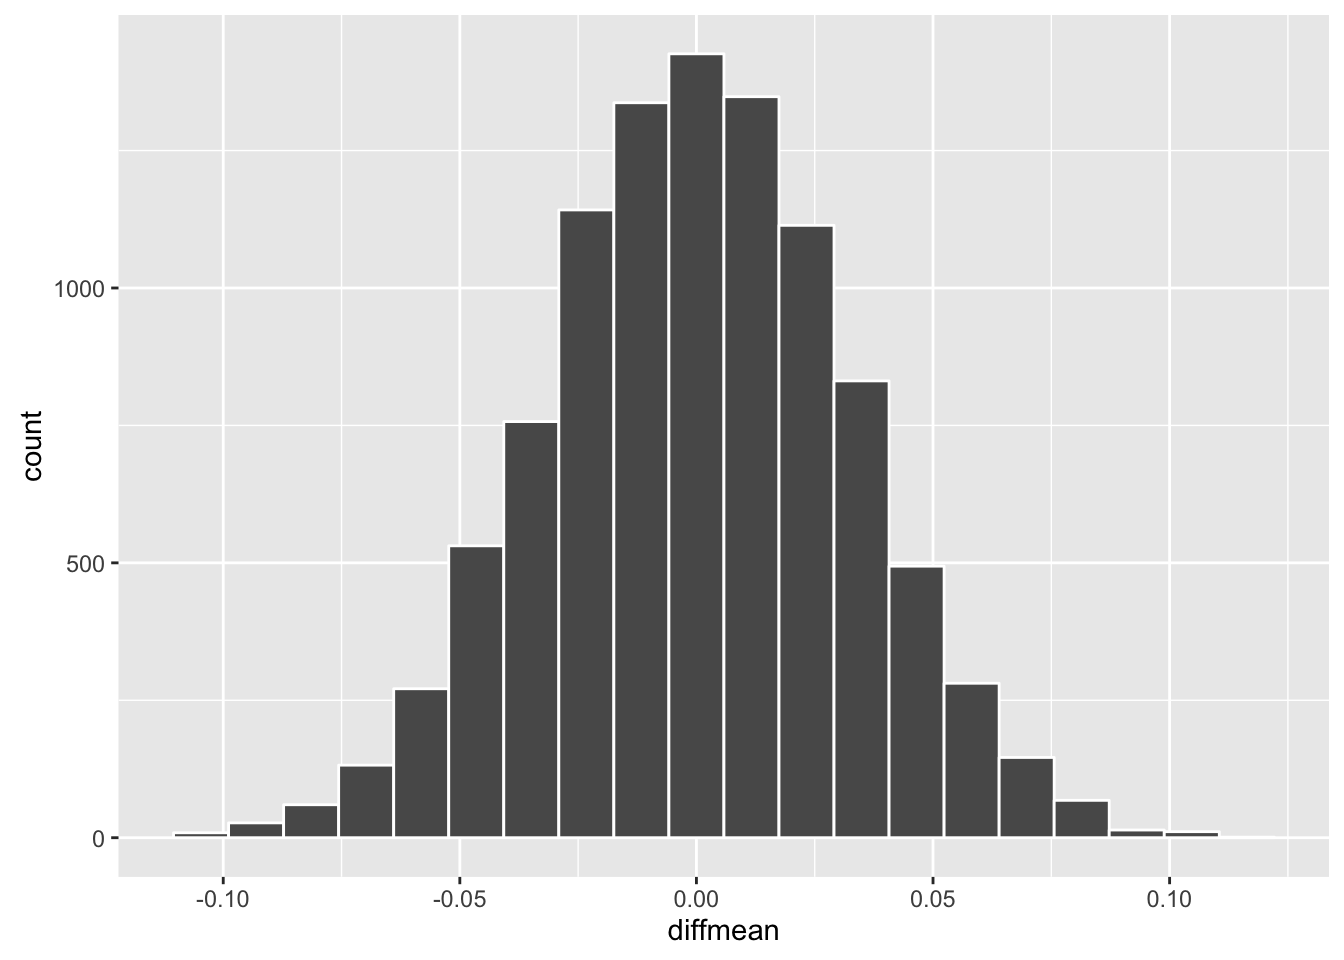
\includegraphics[width=\textwidth]{ismay_files/figure-latex/unnamed-chunk-115-1} 

}

\caption[Number of flights departing NYC in 2013 by airline - Descending numbers]{Number of flights departing NYC in 2013 by airline - Descending numbers}\label{fig:unnamed-chunk-115}
\end{figure}

\begin{Shaded}
\begin{Highlighting}[]
\CommentTok{#ggplot(data = carrier_counts, mapping = aes(x = carrier, y = n)) +}
\CommentTok{#  geom_bar(stat = "identity") + }
\CommentTok{#  scale_x_discrete(limits = carrier)}
\end{Highlighting}
\end{Shaded}

The last addition here specifies the values of the horizontal \texttt{x}
axis on a discrete scale to correspond to those given by the entries of
\texttt{sorted\_flights}.

\section{Interactive graphics}\label{interactive-graphics}

\subsection{Interactive line-graphs}\label{interactive-line-graphs}

Another useful tool for viewing line-graphs such as this is the
\texttt{dygraph} function in the \texttt{dygraphs} package in
combination with the \texttt{dyRangeSelector} function. This allows us
to zoom in on a selected range and get an interactive plot for us to
work with:

\begin{Shaded}
\begin{Highlighting}[]
\KeywordTok{library}\NormalTok{(dygraphs)}
\KeywordTok{rownames}\NormalTok{(flights_summarized) <-}\StringTok{ }\NormalTok{flights_summarized$date}
\NormalTok{flights_summarized <-}\StringTok{ }\KeywordTok{select}\NormalTok{(flights_summarized, -date)}
\KeywordTok{dyRangeSelector}\NormalTok{(}\KeywordTok{dygraph}\NormalTok{(flights_summarized))}
\end{Highlighting}
\end{Shaded}

\begin{center}\includegraphics[width=1\linewidth]{ismay_files/figure-latex/unnamed-chunk-116-1} \end{center}

The syntax here is a little different than what we have covered so far.
The \texttt{dygraph} function is expecting for the dates to be given as
the \texttt{rownames} of the object. We then remove the \texttt{date}
variable from the \texttt{flights\_summarized} dataframe since it is
accounted for in the \texttt{rownames}. Lastly, we run the
\texttt{dygraph} function on the new dataframe that only contains the
median arrival delay as a column and then provide the ability to have a
selector to zoom in on the interactive plot via
\texttt{dyRangeSelector}. (Note that this plot will only be interactive
in the HTML version of this book.)

\chapter{Appendix B: Statistical Basics}\label{appendix2}

\section{Basic statistical terms}\label{basic-statistical-terms}

\subsection{Mean}\label{mean}

The mean is the most commonly reported measure of center. It is commonly
called the ``average'' though this term can be a little ambiguous. The
mean is the sum of all of the data elements divided by how many elements
there are. If we have \(n\) data points, the mean is given by:
\[Mean = \frac{x_1 + x_2 + \cdots + x_n}{n}\]

\subsection{Median}\label{median}

The median is calculated by first sorting a variable's data from
smallest to largest. After sorting the data, the middle element in the
list is the \textbf{median}. If the middle falls between two values,
then the median is the mean of those two values.

\subsection{Standard deviation}\label{standard-deviation}

We will next discuss the \textbf{standard deviation} of a sample data
set pertaining to one variable. The formula can be a little intimidating
at first but it is important to remember that it is essentially a
measure of how far to expect a given data value is from its mean:

\[Standard \, deviation = \sqrt{\frac{(x_1 - Mean)^2 + (x_2 - Mean)^2 + \cdots + (x_n - Mean)^2}{n - 1}}\]

\subsection{Five-number summary}\label{five-number-summary}

The \textbf{five-number summary} consists of five values: minimum, first
quantile (25\textsuperscript{th} percentile), median
(50\textsuperscript{th} percentile), third quantile
(75\textsuperscript{th}) quantile, and maximum. The quantiles are
calculated as

\begin{itemize}
\tightlist
\item
  first quantile (\(Q_1\)): the median of the first half of the sorted
  data
\item
  third quantile (\(Q_3\)): the median of the second half of the sorted
  data
\end{itemize}

The \emph{interquartile range} is defined as \(Q_3 - Q_1\) and is a
measure of how spread out the middle 50\% of values is. The five-number
summary is not influenced by the presence of outliers in the ways that
the mean and standard deviation are. It is, thus, recommended for skewed
data sets.

\subsection{Distribution}\label{distribution}

The \textbf{distribution} of a variable/data set corresponds to
generalizing patterns in the data set. It often shows how frequently
elements in the data set appear.

\subsection{Outliers}\label{outliers}

\textbf{Outliers} correspond to values in the data set that fall far
outside the range of ``ordinary'' values. In regards to a boxplot (by
default), they correspond to values below \(Q_1 - (1.5 * IQR)\) or above
\(Q_3 + (1.5 * IQR)\).

Note that these terms (aside from \textbf{Distribution}) only apply to
quantitative variables.

\bibliography{bib/packages.bib,bib/books.bib,bib/articles.bib}



\end{document}
